%!TEX program=xelatex
%!TEX program=bibtex
%!TEX program=xelatex
%!TEX program=xelatex
% !Mode:: "TeX:UTF-8"
\documentclass[master,openany,twoside,a4paper,AutoFakeBold]{sudathesis}
\usepackage{tikz-dependency}
\usepackage{graphicx}
\usepackage{tikz}
\usepackage{tikz-qtree}
\usepackage{caption}
\usepackage{bbm}
\usepackage{letltxmacro}
\usepackage{mathtools}
\usepackage{pgfplots}
\usepackage{dashrule}
\usepackage[hang,flushmargin]{footmisc} % no indentation for footnotes
%\usepackage[SlantFont,BoldFont,CJKchecksingle,CJKnumber]{xeCJK}
%\setmainfont[BoldFont=SimHei ,ItalicFont=KaiTi_GB2312]{SimKai}
%\newcommand\fontnamekai{KaiTi_GB2312}

\usepackage{graphics}
\usepackage{pdfpages}
\usepackage{array}
\usepackage{tabu}
\usepackage{amssymb}
\usepackage{wasysym}
\usepackage{pifont}
\usepackage{color}
\usepackage{xcolor}
\usepackage{booktabs}
\usepackage{makecell}
\usepackage{tgtermes}


\DeclareMathOperator*{\argmax}{argmax}

\newfontfamily\tgtermes{TeX Gyre Termes}
\makeatletter
  \begingroup
    \tgtermes
    \DeclareFontShape{\f@encoding}{\rmdefault}{m}{sc}{%
      <-> ssub * \f@family/m/sc}{}
    \DeclareFontShape{\f@encoding}{\rmdefault}{bx}{sc}{%
      <-> ssub * \f@family/bx/sc}{}
  \endgroup
\makeatother
\newcommand*\tcircle[1]{%
  \raisebox{.5pt}{\textcircled{\raisebox{-.9pt} {#1}}}
}

\begin{document}

% 论文相关信息
% !Mode:: "TeX:UTF-8"

% 学院中英文名,中文不需要“学院”二字
% 院系英文名可从以下导航页面进入各个学院的主页查看
% http://www.buaa.edu.cn/xyykc/index.htm
\school
{计算机科学与技术学院}{School of Conputer Science and Technology}

% 专业中英文名
\major
{计算机科学与技术~~~}{Computer Science and Technology}

% 方向中英文名
\direct
{自然语言处理~~}{Natural Language Processing}

% 论文中英文标题
\thesistitle
{面向长文本的机器阅读理解研究}{Reasearch on Long Text-oriented Machine Reading Comprehension}

% 作者中英文名
\thesisauthor
{董梦星~~~~}{Mengxing Dong}

% 导师中英文名
\teacher
{洪宇}{Yu Hong}


% 班级
\class{XXXX}

% 学号
\studentID{20204227053}

% 单位代码
\unicode{10285}

% 论文时间,用于首页
\thesisdate{2023}{4}


\maketitle

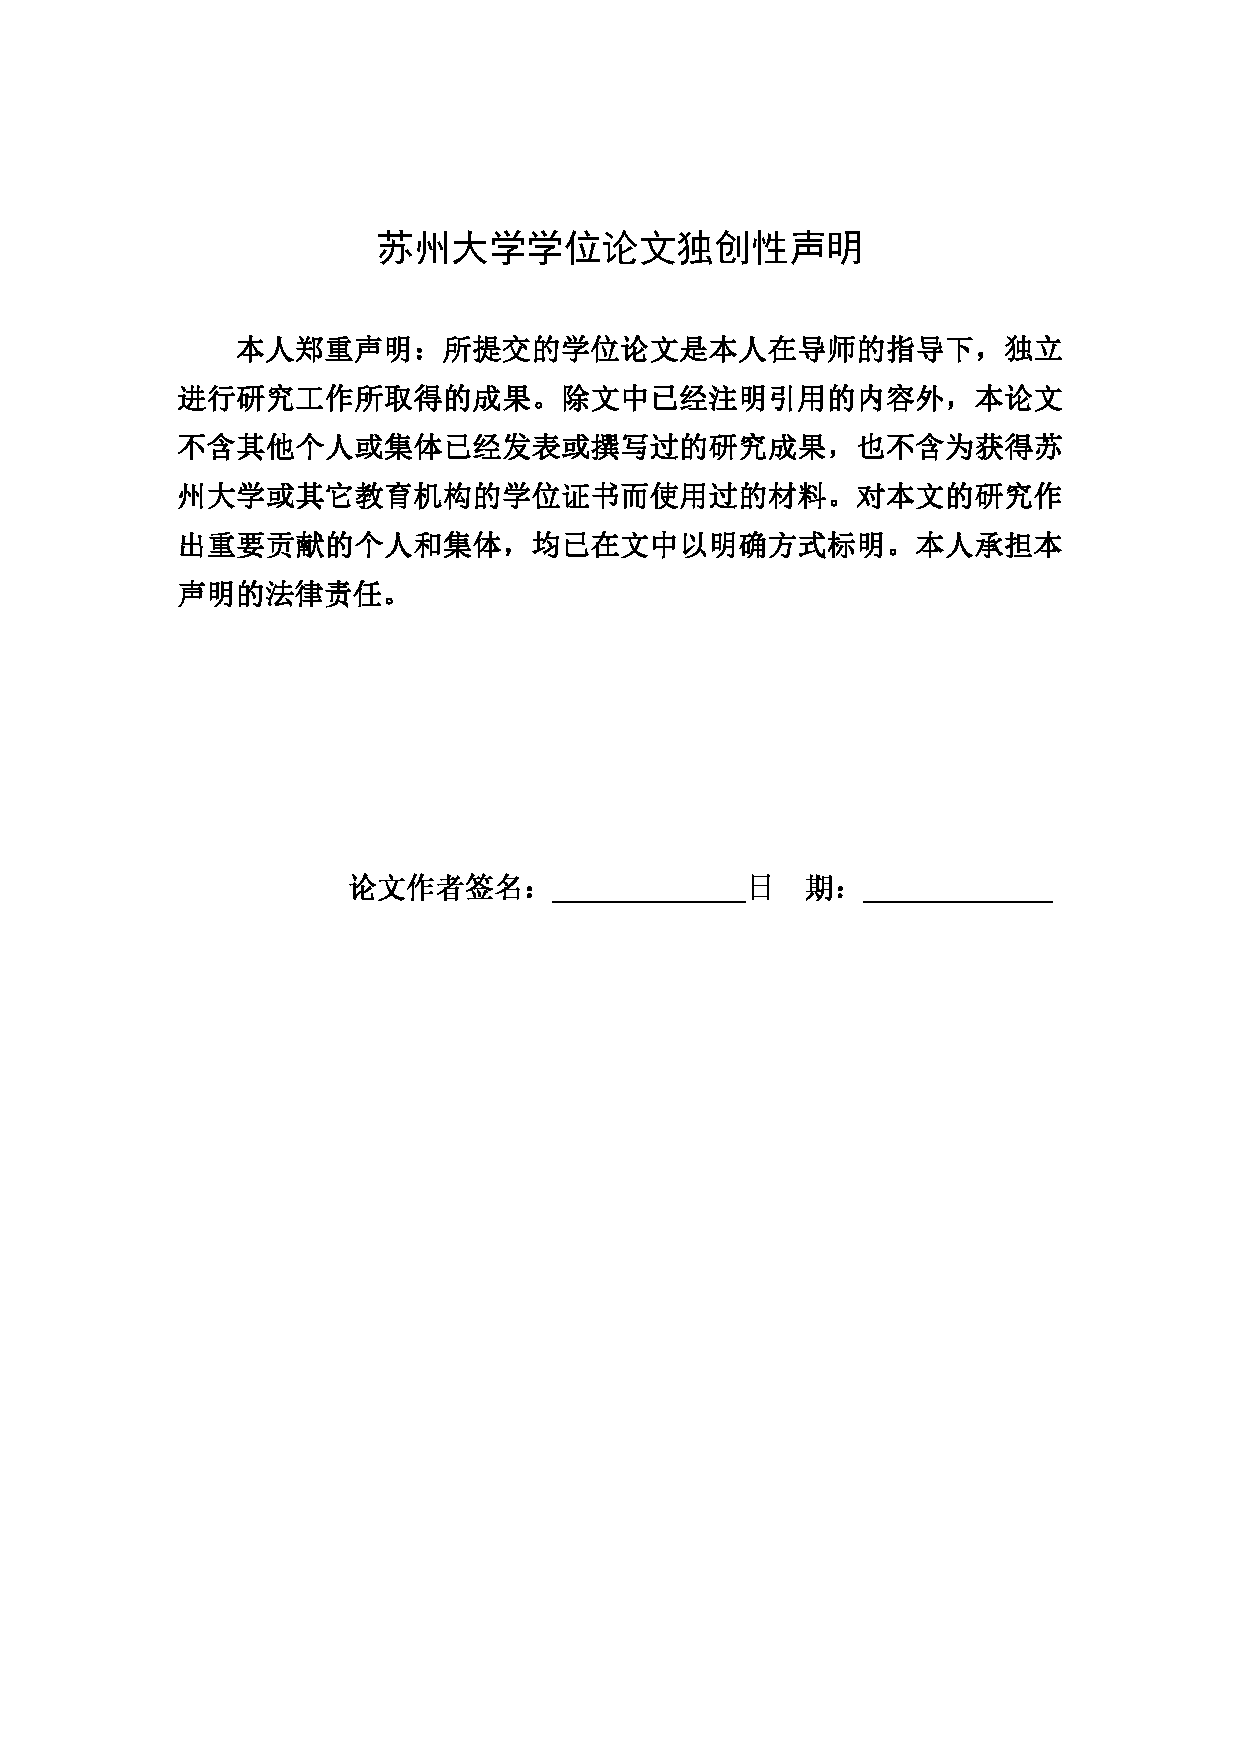
\includepdf[page=-]{pdf-pages/独创性声明.pdf}

\includepdf[page=-]{pdf-pages/空白页.pdf}
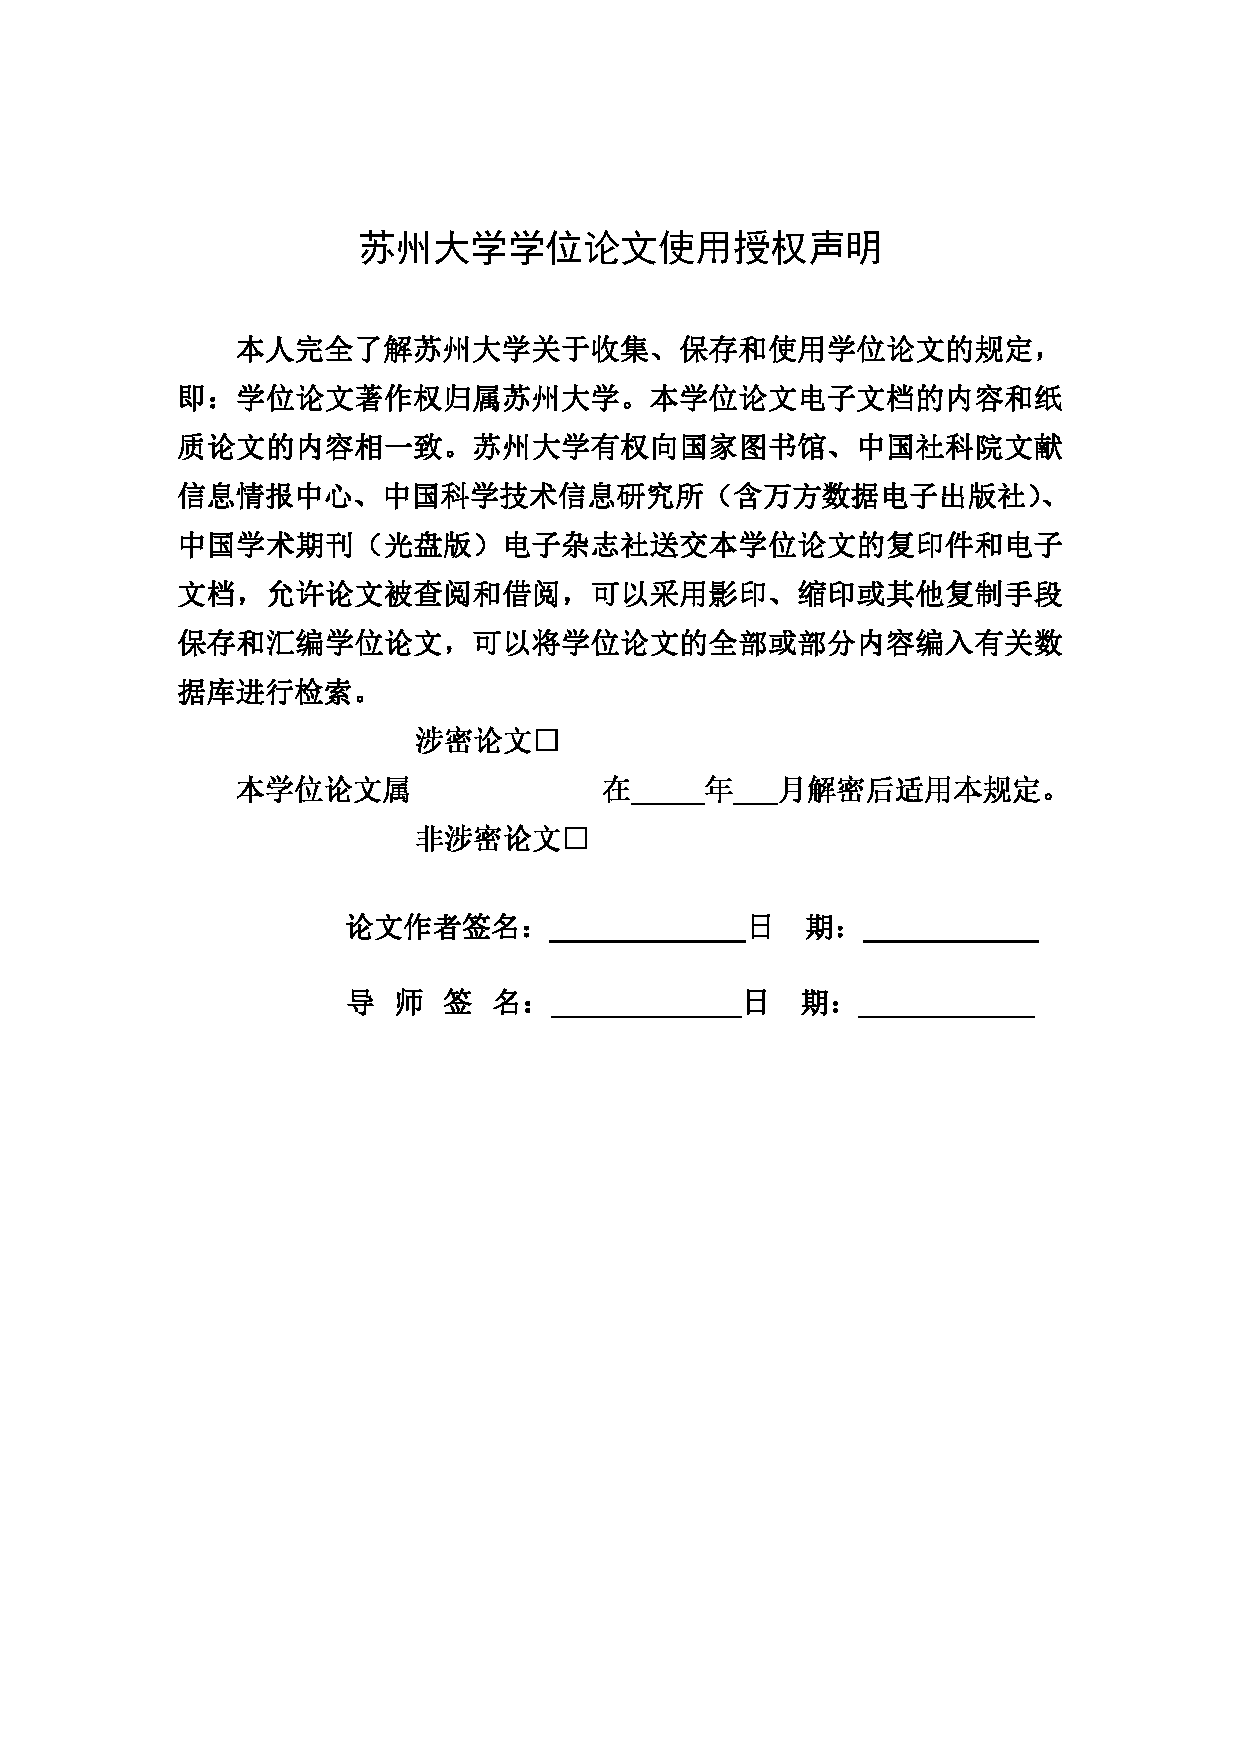
\includepdf[page=-]{pdf-pages/授权声明.pdf}

\includepdf[page=-]{pdf-pages/空白页.pdf}

% 正文前页码是大写罗马字母
\pagenumbering{Roman}
% 前言页眉页脚样式 % 摘要
\pagestyle{cnfrontmatter}
% !Mode:: "TeX:UTF-8"

% 中英文摘要
\begin{cabstract}
    % 长机器阅读理解的定义
    本文旨在探讨面向长文本的机器阅读理解技术,即让计算机程序能够自动阅读长篇文本信息,并以与人类类似的方式理解长文本,随后回答相关问题的能力。
    % MRC的重要性
    这项技术是自然语言处理领域中一个重要的研究方向,并且已经在许多应用场景中发挥了重要作用,例如智能问答、文本摘要、机器翻译和知识图谱构建等。

    % 长文本机器阅读理解的应用
    随着互联网技术的迅速发展,人们面临的文本信息越来越多,包括新闻报道、学术论文等。
    为了更快速、更准确地获取需要的信息,长文本机器阅读理解技术应运而生,并且逐渐成为研究的热点。
    % LT-MRC的重要性
    长文本阅读理解技术涉及多个子任务,如文本分段、关键信息提取、逻辑推理等。为了完成这些任务,需要采用多种自然语言处理技术,如滑动窗口、序列标注等。
    % LT-MRC的挑战
    然而,长文本阅读理解也面临一些挑战。
    首先,长文本中存在大量跨句子和跨段落的逻辑关系,例如条件关系、递进关系等,这些关系需要进行跨句子和跨段落的推理才能正确理解文本意义。
    其次,阅读和理解长文本需要消耗大量的计算资源和时间,因此如何在保证精度的前提下提高效率也是一个难点。

    % LT-MRC的解决方案1
    首先,基于目前领域内最为重要的新闻长文本语料NewsQA,本文提出了一种基于检索器和阅读器二阶段架构的方法。
    该方法基于预训练语言模型,分别实现问题与文本片段的相关性检索,以及进行序列标注,从而抽取答案文本片段。

    % LT-MRC的解决方案3
    第二,现有的长文本阅读理解架构通常只采用检索的方式来获取关键信息。
    本文另辟蹊径,通过在多跳阅读理解数据集MuSiQUe上实验,提出了一种生成式的方法,将多跳问题转化为多个单跳子问题,并依次借助阅读理解模型,提取每个子问题的关键文本段落以及答案片段。

    % LT-MRC的解决方案2
    % 最后,针对长文本多项选择语料QuALITY中,文本与多个备选答案都存在关联的情形下,仅仅依赖问题对文本进行简单的检索,往往忽略了选项存在的重要性。
    % 因此,本文利用问题与备选答案指向的稠密检索器,检索出关键信息。
    最后,针对长文本多项选择语料QuALITY中,文本与多个备选答案都存在关联的情形下,本文利用问题与备选答案指向的稠密检索器,检索出关键信息。
    同时,本文采用对比学习,以及改良过后的样本间自注意力机制,对备选答案进行更准确的语义表示,以解决备选答案之间的密切联系与区别。

    % 总结
    本文的研究目的在于探讨长文本机器阅读理解的方法,通过提取关键信息、备选答案交互以及多跳问题分解等多个角度,本文提出了三种解决方案。通过在多个开源数据集,如NewsQA、QuALITY、MuSiQue上进行实验,本文的方法取得了显著的评测指标提升,说明在长文本阅读理解方面拥有一定的实用价值。
    % 未来,我们仍希望通过不断改进算法和提高数据质量来进一步提高模型的性能和应用范围。	
	\vskip 21bp
	{\heiti\zihao{-4} 关键词:}
	机器阅读理解,
	长文本,
	稠密检索器,
	问题分解
	\begin{flushright}
		作~~~~者:董梦星
		
		指导老师:洪宇
		
	\end{flushright}
\end{cabstract}




\pagestyle{enfrontmatter}
% !Mode:: "TeX:UTF-8"

\begin{eabstract}
	Syntactic parsing is one of the most important intermediate processes in sentence comprehension,
	and probability estimation has always been a core problem in the parsing field.
	However, in either deep learning (DL) era or pre-DL era, there exist very few works based on global probabilistic modeling, mainly due to the high complexity of tree-structure CRF (TreeCRF) inference.
	This thesis proposes to apply TreeCRF to both dependency parsing and constituency parsing.
	The key idea to solve the inefficiency issue is to batchify the inference algorithm for tree structures, and meanwhile avoid the complex Outside algorithm via back-propagation.
	Currently, parsing models are greatly simplified, and it's a trend to adopt local loss for syntactic parsing.
	In contrast, we propose a high-order extension to first-order models.
	While high-order modeling further increases the algorithm complexity, we also try to apply mean field variational inference (MFVI) as an alternative to exact inference of TreeCRF method, which greatly improves the parsing efficiency.

	\vskip 21bp
	{\bf\zihao{-4} Key words: }
	Syntactic Parsing,
	Dependency Parsing,
	Constituency Parsing,
	TreeCRF,
	Variational Inference
\end{eabstract}

\begin{flushright}
	Written by Mengxing Dong
	
	Supervised by Yu Hong
\end{flushright}


% 目录不设置页眉和页码
\makeatletter
\let \asas \ps@plain
\let \ps@plain \ps@empty
\makeatother
\pagestyle{empty}

% 生成目录
\tableofcontents
\setcounter{secnumdepth}{4}

\makeatletter
\let \ps@plain \asas
\let\asas\relax
\makeatother
\clearpage  %目录3页以上,使用cleardoublepage

% 正文页码样式
\mainmatter
% 正文页眉页脚样式
\pagestyle{mainmatter}
% 正文页码是阿拉伯数字
\pagenumbering{arabic}

% % 正文

\chapter{绪论}
本章旨在探讨长文本机器阅读理解的研究背景和意义,并对国内外研究现状的几个主要方面进行介绍,包括机器阅读理解、长文本机器阅读理解和开放域问答。
在此基础上,本章分析了关键科学问题和研究难点。
针对这些关键科学问题,本章详细介绍了本文的研究内容和组织结构。


\section{研究背景和意义}
机器阅读理解(Machine Reading Comprehension,简称MRC)旨在教会机器在理解给定自然语言文本的基础上回答与之相关的问题,一直是自然语言处理(Natural Language Processing,简称NLP)领域极具挑战性的前沿研究之一。

% 机器阅读理解的研究背景
早期的机器阅读理解主要依赖于浅层的自然语言处理技术\cite{Liu2019NeuralMR,Zhang2020MachineRC,Cui2019ASD},如关键词提取\cite{Li2021KeywordEM}、句法分析\cite{Yu2022SSAGNetSA}等,而这些技术忽略了句子之间的逻辑关系以及文本的语境信息。
这些技术可以用于对文本进行初步的处理和分析。

随着深度学习技术的发展,机器阅读理解的研究逐渐转向基于神经网络的方法\cite{hermann2015teaching}。
利用深度学习技术,可以构建端到端的模型,从而更好地捕捉句子之间的关系和语境信息,提高长文本机器阅读理解的准确率。

同时,计算机可以帮助人们自动化地理解和处理大量的文本信息,从而节省时间和精力。
这项技术也可以应用于很多场景,如自动化摘要\cite{Dong2018ASO}、文本分类\cite{Liu2016RecurrentNN}、信息检索\cite{Trabelsi2021NeuralRM}、知识图谱\cite{Lan2021KnowledgeGI}等任务,也可以在教育、医疗、金融、智能客服\cite{Ebersbach2016ArtificialNN}等领域使用,使人们能够更加高效的获取和利用信息。

% 长文本机器阅读理解的研究背景
随着数字化信息的快速发展,人们需要从各种各样的长文本中获取信息。
这包括但不限于新闻报道、学术论文、用户手册以及社交媒体。
但是,长文本中通常涵盖了丰富的信息和细节,这增加了人类理解和提取信息的难度。
因此,长文本机器阅读理解成为一项重要的研究任务,旨在通过计算机技术提高长文本处理的效率和准确性。

长文本机器阅读理解的研究与人工智能技术的发展密切相关。
随着深度学习技术在自然语言处理领域的广泛应用和不断发展,机器阅读理解的研究也取得了显著的进展。
深度学习技术为机器阅读理解任务提供了强有力的支持,使得研究人员可以通过大规模数据训练更加精准和高效的机器阅读理解模型。
这些模型可以有效地帮助人们处理长文本中的信息,从而提高信息处理的效率和准确性。

因此,长文本机器阅读理解的研究背景涉及到多个方面,包括人们对于高效阅读的需求、处理复杂语义的挑战以及深度学习技术的快速发展等。
这些方面共同推动着长文本机器阅读理解的不断发展和进步,使得机器能够更好地理解和处理长文本中的信息。
随着这些领域的不断发展和完善,长文本机器阅读理解技术将在未来得到更加广泛的应用,并且在各个领域中发挥着越来越重要的作用。


\section{国内外研究现状}
本节将从机器阅读理解、长文本机器阅读理解以及开放域问答三个研究视角出发,全面介绍国内外关于面向长文本机器阅读理解任务的相关研究工作。

\subsection{机器阅读理解}
机器阅读理解\cite{hermann2015teaching}是自然语言处理领域的研究热点,近年来在国内外都得到了广泛的关注和研究。

% 国外研究现状
随着各种深度学习技术的引入,机器阅读理解在近年来得到了越来越多的关注和发展。
% 数据集
% SQuAD
早在2015年,斯坦福大学推出了首个个由自然语言问题构成的的大规模机器阅读理解数据集SQuAD\cite{rajpurkar2016squad};
SQuAD数据集的目标是让机器阅读理解模型能够回答自然语言问题,并从给定的篇章中正确地提取出答案。
% SQuAD2.0
继SQuAD数据集之后,研究者们陆续提出了更多具有挑战性的大规模机器阅读理解数据集。
为了提升模型回答的能力,SQuAD2.0\cite{Rajpurkar2018KnowWY}横空出世;
相比于SQuAD,增加了一些负样本,这些负样本包括了那些在篇章中无法找到答案的问题;
因此,SQuAD2.0不仅要求模型回答问题,还需要模型能够判断出问题是否有答案。
% NewsQA
NewsQA\cite{trischler2016newsqa}也是一个类似于SQuAD的大规模机器阅读理解数据集,专注于新闻文章的阅读理解,其中包括来自CNN和Daily Mail等新闻网站的超过10,000篇新闻文章。
% RACE
此外,多项选择式机器阅读理解数据集RACE\cite{lai2017race},类似于中国学生参加的中考和高考英语,收录了来自高中和大学英语考试中的阅读理解题目;
RACE数据集中的问题包含多种类型,涵盖了不同难度级别,既有简单的词汇理解,也有复杂的推理和推断。
% HotpotQA
基于多跳推理的大规模机器阅读理解数据集HotpotQA\cite{Yang2018HotpotQAAD},要求模型搜索多个文档的信息,回答一系列问题;
由于涉及多个文档信息,HotpotQA需要模型进行多文档联合推理。

% 模型
与此同时,伴随着大规模机器阅读理解数据集的问世,基于神经网络的机器阅读理解模型也相继涌现。
基于神经网络的机器阅读理解模型大多采用嵌入层,编码层,交互层和输出层等四层架构。
% BiDAF
BiDAF\cite{Seo2016BidirectionalAF}最早实现了双向注意力流机制,将问题与文本之间的语义关联性建模为一个注意力矩阵;
并且通过引入字符级别的编码器,增强了模型对于语言的理解能力和语义建模能力。
% Reasonet
基于知识图谱的机器阅读理解模型Reasonet\cite{Shen2016ReasoNetLT},通过将知识图谱中的实体和关系引入到机器阅读理解模型中,来提高模型的推理能力和文本理解能力。
% QANet
基于卷积神经网络的QANet\cite{Yu2018QANetCL},使用自注意力机制来学习文章和问题之间的交互表示,捕捉文章中与问题相关的信息,从而更有效的处理长文本和多文档场景。
这些模型大多基于深度学习技术,通过对大规模数据的学习来提高阅读理解的能力。
% Match-LSTM
此外,基于多层LSTM的模型Match-LSTM\cite{Wang2016MachineCU},可以同时对上下文和问题进行建模,并使用注意力机制来对匹配信息进行加权。
% BERT
在Transformer架构发布之后,研究人员陆续提出了各种预训练语言模型,例如BERT\cite{devlin2018bert}、RoBERTa\cite{liu2019roberta}、DeBERTa\cite{he2021debertav3}等,并在各种机器阅读理解任务上取得了成功。
这些预训练语言模型极大地推进了自然语言处理领域的发展,它们的成功很大程度上归功于它们能够通过对大规模语料库的无监督预训练学习到文本的丰富表示。
因此,本文提出的面向长文本的机器阅读理解方法均基于预训练语言模型进行开研究与开发。

% 国内研究现状
与此同时,国内研究者在机器阅读理解领域也取得了一定的进展。
% 数据集
一些国内高校和科研机构也相继推出了机器阅读理解数据集和模型。
% 清华大学
清华大学自然语言处理与社会人文计算实验室提出的中文机器阅读理解数据集CMRC\cite{Cui2019ASD},涵盖了新闻、百科、论坛等不同类型的文本,同时考虑了答案的多样性和篇章的连贯性。
% 百度
百度提出的中文机器阅读理解数据集DuReader\cite{He2017DuReaderAC},囊括了答案抽取问题,以及选择题;
该数据集在答案抽取和篇章连贯性方面的研究具有重要意义。
% 华为
华为也针对汉语语言提出了CLUER-MRC\cite{xu2020clue}等四个相关的中文机器阅读理解数据集。

% 方法
除了数据集的构建外,中文机器阅读理解方面的研究还包括了一系列的方法探索和技术创新。
% Chinese Machine Reading Comprehension Based on Language Model Containing Knowledge
Wentong\ Chen等人\cite{Chen2022ChineseMR}提出了一种利用预训练的语言模型来提高中文机器阅读理解性能的方法,同时考虑了人类在理解文本时会关联的一些外部相关知识;
该工作在BERT模型的基础上,引入了一个知识库模块,用于从给定的问题和上下文中抽取相关知识,并将其融合到语言模型中。
% Machine Reading Comprehension Model Based on Multi-head Attention Mechanism
Xue等人\cite{xue2022machine}提出了一种基于多头注意力机制的机器阅读理解模型,能有效的捕捉中文文本和问题之间的关系。


\subsection{长文本机器阅读理解}
长文本机器阅读理解是在机器阅读理解的基础上,把输入文本换成了更长的形式。
长文本阅读理解需要更强的对上下文和语境的理解能力,并且需要解决长文本中的信息丰富性、篇章结构复杂等挑战。
如今,国内外研究者们都在积极探索这个问题,并取得了一些进展。

% 数据集
% TriviaQA
TriviaQA\cite{Joshi2017TriviaQAAL}是一个长文本机器阅读理解数据集,其问题和文本来自于维基百科、Web网页等多个知识来源,文本长度有很大的变化范围,短至几百个单词,长可达几千甚至上万个单词;
该数据集的发布推动了长文本机器阅读理解任务的研究,并成为该领域研究的重要基准数据集之一。
% NarrativeQA
NarrativeQA\cite{Kocisk2017TheNR}是一个包含大量小说和电影剧本的数据集,用于自然语言处理和长文本机器阅读理解研究。

% 国内外研究现状
% 滑动窗口
关于长文本的处理方法,滑动窗口\cite{joshi2019bert}机制是一种常用的技术,它将长文本分割成多个较小的片段,以便于模型处理。
% A Thorough Examination of the CNN/Daily Mail Reading Comprehension Task
Danqi\ Chen等人\cite{Chen2016ATE}最早使用滑动窗口技术将长篇新闻文章分成多个段落,然后使用卷积神经网络模型进行阅读理解。
% Machine Comprehension Using Match-LSTM and Answer Pointer
随后,滑动窗口技术被广泛应用于长文本机器阅读理解任务中。
例如,Shuohang Wang等人\cite{Wang2016MachineCU}将长文本切分成多个窗口,并使用基于LSTM和注意力机制的模型来处理每个窗口,最终预测答案。
% R-Net: Machine Reading Comprehension with Self-Matching Networks
Wang Wenhui等人\cite{wang2017r}也采用滑动窗口技术来处理长文本,然后使用自匹配注意力网络\cite{Wang2017GatedSN}(Self-matching Networks)来捕捉文本之间的交互信息。
% DPR
除了这种方法,Facebook AI Research在2018年提出了稠密向量检索\cite{Karpukhin2020DensePR}(Dense Passage Retrieval, 简称DPR),它是一种从大规模文本集合中检索出最相关的文本段落的检索技术;
DPR利用双塔结构将文本表示为向量,并通过检索候选文本库的方式来处理长文本机器阅读理解问题。
此后,DPR被广泛应用于TriviaQA,Natrual Questions等多个数据集,并取得了很好的效果。
% Transformer-XL
此外,Transformer-XL\cite{Dai2019TransformerXLAL}在基于Transformer\cite{vaswani2017attention}语言模型的基础上,引入了递归机制和相对位置编码来解决长文本的问题;
递归机制允许模型在处理长序列时保留之前的状态信息;
相对位置编码技术允许模型在处理长文本时捕捉到相对位置的信息。
% CogLTX
国内研究者们也在长文本机器阅读理解领域进行了很多探索和实践。
清华大学和阿里巴巴联合提出了一种基于认知理论的框架CogLTX\cite{Ding2020CogLTXAB},可以将BERT等预训练语言模型应用到长文本上;
CogLTX通过训练一个判断模型来识别长文本中的关键句子,并将其串接进行推理,并通过排练和衰减实现多步骤推理。


\subsection{开放域问答}
开放域问答\cite{allam2012question}(Open Domain Question Answering)是一种自然语言处理任务,旨在从大规模的自由文本中回答人类提出的自然语言问题。
它通常包含信息检索和阅读理解两个子任务。
由于其自由文本的语言表达方式和信息组织方式多样,开放域问答技术通常要求模型具有对多样化文本的理解、推理和组织能力。
开放域问答技术通常可以用于搜索引擎当中,如今很多国内外学者都在研究这一技术的应用与创新。

% 数据集
% Natural Question
Natural Questions\cite{Kwiatkowski2019NaturalQA}(NQ)是由Google推出的一个开放域问答数据集,它是一个基于真实用户提问和真实网页文本的数据集;
NQ信息检索任务要求系统仅通过问题,从真实网页中选择一个最相关的文档。
% SearchQA
SearchQA\cite{Dunn2017SearchQAAN}是一个基于搜索引擎的开放域问答数据集,其中由超过140,000个人工制作的问题来自于人们在真实的搜索引擎中提出的查询;
该数据集的特点是问题的多样性和复杂性,其中包括一些需要深入理解文化、历史和常识的问题。

% 国内外研究现状
% Open Domain Question Answering Using Early Fusion of Knowledge Bases and Text
% Pipeline方法作为最早针对开放域问答的方法,类似搜索引擎的工作原理,将开放域问答分为Query理解,候选召回和答案抽取等部分。
Dheeraj Rajagopal等人\cite{Sun2018OpenDQ}提出了一种Pipeline的方法,来解决开放域问答任务中的挑战。
具体来说,该方法首先使用TF-IDF\cite{SprckJones2021ASI}等技术对文本进行编码,然后使用知识库中的实体和属性对编码进行扩展,以便更好地捕获问题和答案之间的语义关系;
接下来,该方法使用文本和知识库中的信息进行匹配和排序,并使用基于规则和基于机器学习的技术来生成答案。
% Reading Wikipedia to Answer Open-Domain Questions
另一种称为“两阶段方法”的流程是,首先使用检索器对大量给定的文档进行筛选,从中提取与问题相关的部分文本片段,然后从这些文本片段中抽取出答案。
Danqi Chen等人\cite{Chen2017ReadingWT}提出了一种新的方法,使用预训练语言模型来代替传统的阅读理解模型,对Wikipedia的文章进行阅读和理解,从中抽取问题相关的段落和答案。
% ORQA: Open Retrieval Question Answering
部分科研工作采用了端到端学习的方式,将检索器和阅读器模型同时进行训练,从而实现更加紧密的模型集成和协同工作。
其中一个典型例子是ORQA\cite{lee2019orqa},该方法通过联合训练检索器和阅读器,实现了对候选文档的精细筛选和对答案的精准抽取,从而提高了整个Pipeline的效率和准确性。
% How Much Knowledge Can You Pack Into the Parameters of a Language Model?
也有一些大模型,甚至可以不进行微调,而直接预测答案。
Adam Roberts等人\cite{Roberts2020HowMK}探讨了神经语言模型在无结构文本上训练时能够隐式地存储和检索知识的能力,并提出了一种评估方法来测量模型参数中包含的知识量。


\section{关键问题和研究难点}
机器阅读理解可以应用于多种自然语言处理任务,其具有重要的理论意义和广阔的应用前景。
如今,以预训练语言模型为主的神经机器阅读理解技术得到了快速发展,但机器阅读理解模型在长文本问答场景下仍有巨大的提升空间。

% 关键问题
长文本机器阅读理解的关键问题和研究难点主要包括以下几个方面:

% 问题理解
(1)问题理解

多文档机器阅读理解\cite{song2019multi}是长文本机器阅读理解的一种形式,其与传统的阅读理解任务相比,需要更深入的理解和推理。
该任务中问题的多跳形式使得问题的语法结构和包含的内容信息非常复杂,这使得神经网络模型在理解问题时面临许多挑战。
例如,模型需要理解问题中的关键信息和上下文,并能够识别问题中不同子问题之间的联系和顺序,以便逐步构建问题的完整解答。
问题理解的难点在于需要将自然语言转换为计算机可以理解的形式,同时还需要在不丢失关键信息的前提下对问题进行简化,以提高模型的理解能力。

为了解决这个问题,研究者们提出了各种不同的方法,包括基于图神经网络\cite{ding2019cogqa}的方法、基于知识库\cite{Luo2018KnowledgeBQ}的方法、基于语义\cite{zhang2021skeleton}的方法和基于转换\cite{Tu2019MultihopRC}的方法等。
这些方法都旨在提高模型对问题理解的能力,以实现更加准确和智能的多文档机器阅读理解。

% 段落或文档检索
(2)文档选择

在长文本机器阅读理解任务中,有时需要从大量的文档或段落中选择与问题相关的文档进行阅读理解。
如果直接将所有文档都送入神经网络模型进行处理,会导致计算代价过大,同时降低模型的准确性和鲁棒性。
因此,文档选择成为了长文本机器阅读理解任务中的一个关键问题,其目标是从候选文档集中快速且准确地筛选出与问题相关的文档,以减少计算代价和提高精度。

文档选择的难点在于如何有效地区分候选文档中与问题相关的内容和无关的内容。
这需要模型能够理解问题的意义和背景,并能够识别出文档中与问题相关的段落和句子。
现有的文档选择方法包括基于特征\cite{Severyn2015LearningTR}的方法、基于深度学习\cite{wu2017sequential}的方法和基于知识库\cite{Luo2018KnowledgeBQ}的方法等。
这些方法尝试从不同的角度对文档进行建模,以便更好地捕捉与问题相关的信息。
% 例如,基于深度学习的方法可以利用神经网络自动学习文档和问题之间的语义联系,而基于知识库的方法可以利用外部知识库中的知识来指导文档选择。
此外,研究者们还尝试了多阶段的文档选择\cite{Gan2019MultistepRV}方法,通过逐步缩小候选文档集的规模来提高文档选择的准确性和效率。

% 答案抽取
(3)答案抽取

机器阅读理解中的答案抽取是指如何从选出的相关段落中准确地抽取出符合问题要求的答案,以满足用户需求和提高质量。
% 其存在一些难点。
% 答案抽取是长文本机器阅读理解任务中的关键步骤之一,其目的是从选出的相关段落中准确地抽取出符合问题要求的答案。
这个过程不仅涉及到答案的位置定位,还需要对答案进行语义理解和答案类型判断等\cite{Zhou2021AnOD},以满足用户需求并提高阅读理解质量。

然而,答案抽取过程中存在一些难点。
首先,答案往往需要从复杂的文本结构中抽取,涉及到不同语言学层面的分析和理解,如词汇、句法和语义等\cite{Sordoni2015ANN,Moschitti2008KernelsOL,Thomas2022AnAH}。
这需要模型具备深厚的自然语言处理能力,能够理解文本中的逻辑关系和上下文信息,同时能够处理诸如命名实体识别和语义角色标注等任务\cite{Shi2019SimpleBM,Lample2016NeuralAF}。
其次,文本中可能存在歧义和多义性,同一问题可能有多个可能的答案,因此模型需要具备有效的答案排序和评估机制\cite{cui-etal-2020-multi}。
在答案抽取的过程中,模型还需要考虑多个相关段落中的答案,并进行合并和消歧。
最后,还需要考虑多种类型的问题,如开放式问题和封闭式问题等。
不同类型的问题对于答案抽取的难度和挑战也不同,因此需要针对不同类型的问题选择合适的答案抽取方法\cite{Zhang2016QuestionAO}。

% 总结
总之,长文本机器阅读理解是自然语言处理领域的一个重要研究方向,其涉及到多个复杂的子任务,如问题理解、文档选择、答案抽取等,每个子任务都存在着一些独特的难点和挑战。
解决这些难点不仅可以提高机器阅读理解的准确度和效率,还可以促进自然语言处理领域的发展。


\section{研究内容与组织结构}
针对以上总结出的关键问题与研究难点,本节首先引出本文的主要研究内容,随后给出文章的组织结构。

\subsection{研究内容}

% 整体任务结构
\begin{figure}
    \centering
    \includegraphics [width=1.0\textwidth] {figure/1-1.pdf}
    \caption{面向长文本的机器阅读理解研究框架图} 
    \label{fig:1-1}
\end{figure}


本文分别针对段落选择、多跳问题分解、答案选项融合等三个关键问题进行研究,对阅读理解模型进行改进。
针对上述关键问题,本文提出了一种面向长文本的机器阅读理解研究方法,其框架图如图~\ref{fig:1-1}~所示,具体分为以下三个方面:

% 面向新闻长文本的阅读理解研究
(1)基于检索器-阅读器二阶段架构的长文本阅读理解研究

在长文本阅读理解任务中,传统的滑动窗口机制限制于每次只能处理512个词,难以建立长距离依赖,并且在截断部分时会丢失信息。
因此,本文提出了一种基于二阶段架构的解决方案,该方案首先选出证据,然后抽取答案片段。
在第一阶段中,检索器为每个文本片段打分,依据可回答性标签来对文本片段进行排序。
第二阶段中的阅读器从高置信文本片段堆中抽取答案。
这种方式可以在提取精炼信息的前提下进行答案抽取,缩小答案搜索范围,提高答案抽取的准确性。

% 基于问题分解的多跳长文本阅读理解研究
(2)基于问题分解的多跳长文本阅读理解研究

在多文档阅读理解任务中,由于问题过于复杂,且传统的机器阅读理解模型缺乏多跳推理能力,因此本研究提出了两种解决方案来将多跳问题分解为单跳问题。
第一种方法是使用序列到序列的生成式模型\cite{Lewis2019BARTDS,Ni2021SentenceT5SS}将多跳问题转化为多个单跳问题,并用检索模型和阅读理解模型分别筛选最佳文档,抽取最佳答案。
第二种方法是在每次生成当前问题时,利用前驱问题和前驱答案来引导生成过程,并通过检索模型和阅读理解模型抽取单跳问题的答案,直至遇到带有结束标志的单跳问题。
这两种方法可以有效地解决多文档阅读理解任务中的问题复杂性和推理能力缺失问题。

% 基于对比学习的多选长文本阅读理解研究
(3)基于对比学习的多项选择长文本阅读理解研究

在多项选择阅读理解任务中,由于部分干扰选项与正确选项在字面表述上过于相似,同时各个选项在编码阶段缺乏交互,因此存在着正确率偏低的问题。
为此,本文提出采用对比学习方法\cite{gao2021simcse},增强选项文本的编码表示能力,以提高选项的区分度;
同时利用样本内自注意力交互机制\cite{vaswani2017attention},建立多个选项之间的联系,从而使各个选项之间的编码能够相互影响,提高答案的准确性。

\subsection{组织结构}
本文共分为六个章节,论文组织结构和各个章节的主要内容如下:

% 第一章
第一章 绪论。
本章主要介绍长文本阅读理解研究的背景和意义,通过对国内外研究现状的分析,总结目前长文本阅读理解存在的问题和研究难点。
同时,本章还针对论文的研究内容和组织结构进行介绍。

% 第二章
第二章 任务定义和评价方法。
本章首先阐述了面向长文本的机器阅读理解任务的定义,并从样本分布和语言风格等角度对三个不同数据集进行了详细的实验语料资源分析,以此为基础对长文本机器阅读理解进行研究。
最后,本章对长文本阅读理解任务的性能评价指标进行了探讨。

% 第三章
第三章 基于检索器-阅读器二阶段架构的长文本阅读理解研究。
本章针对长文本阅读理解领域,提出了一种基于检索器-阅读器二阶段架构的方法。
该方法首先通过检索器,利用问题与文本片段之间的相关性,筛选出最有可能包含答案的一些文本片段。
接着,通过阅读器,采用当前比较先进的预训练语言模型,从这些精简后的文本片段中抽取最终的答案片段。

% 第五章
第四章 基于问题分解的多跳长文本阅读理解研究。
本章针对多文档阅读理解领域,提出了一种利用问题分解技术来简化问题的方法。
该方法通过使用序列到序列的生成式模型,将复杂的多跳问题分解为多个单跳问题。
然后,利用检索模型和阅读理解模型分别筛选出支持文档,并从中抽取最佳答案。

% 第四章
第五章 基于对比学习的多项选择长文本阅读理解研究。
本章针对多项选择长文本阅读理解领域,提出了一种以对比学习为主的研究方法。
该方法首先通过稠密向量检索的方式,从长文本中筛选出与问题和选项相关的文本片段。
接着,在阅读器中引入了样本内自注意力机制,以增强多个选项之间的交互,并应用对比学习方法来提高文本的表示能力。

% 第六章
第六章 总结和展望。
本章对全文工作进行全面的总结,并对未来的研究方向进行展望。



\chapter{任务定义及评价方法}
% 机器阅读理解是什么
机器阅读理解是指让计算机能够像人类一样理解和回答自然语言文本中的问题,它是自然语言处理技术中的一个重要分支。
机器阅读理解是指让机器模拟人类阅读理解的能力,即让机器能够自动地从文本中抽取出问题的答案。
它是自然语言处理中的一个重要任务。
几年来,将预训练语言模型应用于机器阅读理解任务中,已经取得了很好的效果。

% 长文本机器阅读理解是什么
长文本机器阅读理解是在机器阅读理解的基础上进一步发展,以解决输入长文本篇幅的问题。
这项技术在处理大量长文本时具有重要价值,能够帮助机器有效提取和分析文本中的信息和关系,从而节省人工阅读和分析的时间和成本。
随着数字化时代和互联网的兴起,人们面临的信息量越来越大,长文本机器阅读理解技术可以帮助人类更好地理解和利用这些信息。
此外,该技术还可以整合更多信息和背景知识,以提高智能问答和文本自动生成等应用的准确性和效率。
然而,长文本机器阅读理解也面临着挑战,例如长文本中存在大量的自然语言表达的多样性和歧义,需要机器具备处理这些多义性和歧义性的能力,以正确理解文本的含义。
此外,长文本还涉及到大量上下文信息和推理过程,需要机器具备对上下文信息的理解和推理能力。

% 本文是如何做研究的
本文旨在解决长文本阅读理解领域的共性问题和各个细分领域的难点,基于不同领域的长文本数
据集,提出了三种不同的方法。
本章将详细介绍面向长文本的机器阅读理解的任务定义,实验过程中所采用的的语料,以及该任务的相关评价指标。

\section{任务定义}
长文本机器阅读理解的任务定义等同于常规的机器阅读理解,可以表述为:
给定一个篇幅较长的文本文档$D$(Document)和一个问题$Q$(Question),目标是输出与该问题$Q$相关的文本片段或答案$A$(Answer)。
假设文本文档$D$表示为一个由$n$个单词组成的序列$D = [w_1, w_2, ..., w_n]$\footnote{一般来说,在$n$大于512的情形下,文档$D$可以称之为长文本,本文研究的数据集皆符合这一条件。同时,为了增加文本长度造成的挑战,我们在后两项研究中大幅增加了文本长度。}。
%通常,长文本阅读理解模型需要将该长文本截取为一个由m个单词组成的短文本序列$C = [u_1, u_2, ..., u_m]$。
问题$Q$表示为一个由$m$个单词组成的序列$Q = [q_1, q_2, ..., q_m]$,那么机器阅读理解的任务可以数学化的表示为:
% $\hat{a} = \operatorname*{argmax}_{a \in A} \operatorname{sim}(f_D(D), f_Q(Q, a))$

$$A = f(D, Q)$$

公式中的$f$是一个需要让机器去学习的预测函数,通过向函数$f$提供文本文档$D$和问题$Q$,预测出答案$A$。
根据答案风格和表现方式的不同,长文本机器阅读理解任务可以归纳为以下三种类型\footnote{实际上,机器阅读理解任务按照答案类型可以分为抽取式、生成式、完形填空和多项选择四种,本文的实验数据采用了NewsQA,MuSiQue和QuALITY,分别为抽取式和多项选择类型的答案,并涉及了生成式的方法。因此,本文主要考虑这三种类型的机器阅读理解任务。}:

\begin{table}[htbp]\scriptsize
    \centering
    \caption{长文本阅读理解样例}
    \begin{tabular}{p{48pt}|p{360pt}}
         % \hline
         \multicolumn{2}{c}{\bfseries (1)抽取式样例} \\
         \hline
         文章 & (...) A high court in northern India on Friday acquitted a wealthy businessman facing the death sentence for the killing of a teen in a case dubbed ``the house of horrors.'' Moninder Singh Pandher was sentenced to death by a lower court in February. (...) \\
          & <译文:(...) 上周五,印度北部的一家高级法院宣布无罪释放了一位被指控在一起被称为“恐怖之家”的案件中杀害一名青少年的富商,他曾被下级法院判处死刑。 Moninder Singh Pandher在二月份被下级法院判处死刑。(...) > \\
         \hline
         文本长度 & 644 \\
         \hline
         问题 & When was Pandher sentenced to death?  \\
          & <译文:Pandher何时被判死刑? > \\
         \hline
         答案 & February  \\
          & <译文:二月 > \\
         \hline
         \multicolumn{2}{c}{\bfseries (2)生成式样例} \\
         \hline
         文章 & (...) She took off her old leather shoes and tried on the silver ones, which fitted her as well as if they had been made for her. Finally she picked up her basket. ``Come along, Toto'' she said. ``We will go to the Emerald City and ask the Great Oz how to get back to Kansas again.'' (...) \\
          & <译文:(...) 她脱下旧皮鞋试穿上那双银鞋,它们非常适合她,好像是为她量身定制的一样。最后她拿起篮子,“走吧,托托,”她说,“我们去祖母城问伟大的奥兹怎样才能回到堪萨斯。” (...) > \\
         \hline
         文本长度 & 32,655 \\
         \hline
         问题 & Why does Dorothy want to go home? \\
          & <译文:为什么Dorothy想要回家?> \\
         \hline
         答案 & Because she misses her family and friends.  \\
          & <译文:因为她想念她的家人和朋友。> \\
         \hline
         \multicolumn{2}{c}{\bfseries (3)多项选择样例} \\
         \hline
         文章 & (...) ``The Adventure of the Speckled Band'' is one of the 56 short Sherlock Holmes stories written by Sir Arthur Conan Doyle. It was first published in 1892. The story tells how Sherlock Holmes and Dr. Watson investigate the mysterious death of Julia Stoner, the sister of their client Helen Stoner, at Stoke Moran Manor. (...) \\
          & <译文:(...) 《斑点带的冒险》是由亚瑟·柯南·道尔爵士所写的56个短篇福尔摩斯侦探小说之一,首次出版于1892年。故事讲述了福尔摩斯和华生博士调查客户海伦·斯通纳的姐姐朱莉娅·斯通纳在斯托克·莫兰庄园的神秘死亡事件。 (...) > \\
         \hline
         文本长度 & 6,633 \\
         \hline
         问题 & Why did Roylott want to kill Helen?  \\
          & <译文:(...) 为什么Roylott想杀死Helen? (...) > \\
         \hline
         选项 & A. Because he wanted to inherit their mother’s fortune \\ 
         & <译文:因为他想要继承他们母亲的财产。> \\
          & B. Because he wanted to marry Helen; \\
          & <译文:因为他想和Helen结婚。> \\
          & C. Because he wanted to sell Helen to a circus; \\
          & <译文:因为他想把Helen卖到马戏团。> \\
          & D. Because he wanted to use Helen for experiments. \\
          & <译文:因为他想用Helen做实验。> \\
         \hline
         答案 & A \\
         \hline
    \end{tabular}
    \label{tab:2-1}
\end{table}


(1)抽取式(Extractive)

抽取式阅读理解任务是指给定一篇文本和一个问题,模型需要从给定的文本段落中“抽取”出正确的答案片段来回答问题。
抽取式阅读理解实际上是一个分类问题,它要求机器预测答案的开始位置$pos_{start}$与结束位置$pos_{end}$。
最终答案可以表示为$D[pos_{start}:pos_{end}+1]$。
如表~\ref{tab:2-1}~中的抽取式样例所示,列举了NewsQA数据集中的一个样例。
对于问题“When was Pandher sentenced to death?”,答案“February”对应文档中的一个连续的自然文本片段。

(2)生成式(Generative)

生成式阅读理解要求机器基于给定的文本和问题,生成一个合适的答案,该答案不局限于文章中存在的词语,而是自由生成的。
这种任务更适合实际生活场景,但是由于生成的句子无法做准确评估,因此一直无法成为业界的主流数据集。
如表~\ref{tab:2-1}~中的生成式样例所示,列举了NarrativeQA数据集中的一条数据。
对于问题“Why does Dorothy want to go home?”,答案“Because she misses her family and friends.”可以不是文档中的一个连续的文本片段,而是一个自由阐述的文本观点。

(3)多项选择(Multiple Choice)

多项选择阅读理解要求机器基于给定的文章和问题,从多个备选答案中选择一个最有可能是正确答案的选项。
这种任务类似于英语考试中的阅读理解选择题。
当前处理这类问题的模型基本都采用<问题,文章,答案>三元组的框架。
如表~\ref{tab:2-1}~中的多项选择样例所示,列举了QuALITY数据集中的一个样例。
对于问题“Why did Roylott want to kill Helen?”和四个候选答案,机器需要从这四个答案中选出最合适的一个。


\section{语料资源}
本文在新闻长文本阅读理解数据集NewsQA,多跳多文档阅读理解数据集MuSiQue,以及多项选择长文本阅读理解数据集QuALITY三个公开语料上进行相关实验。
本节将分别介绍这三个数据集的详细信息。

\subsection{长文本数据集NewsQA}
% 概述
NewsQA是由纽约大学、卡耐基梅隆大学和麻省理工学院联合推出的一个大规模新闻阅读理解数据集。该数据集覆盖了新闻报道中的多个主题和事件,涉及政治、经济、文化等各个领域,旨在为机器阅读理解任务提供具有挑战性的现实世界应用场景。

% 样本分布(长度、数量等)
(1)样本分布

NewsQA数据集包括超过10,000篇新闻文章,以及超过100,000个与这些文章相关的问答对。
其训练/开发/测试集的分布如~\ref{tab:2-2}~所示。
此外,表格中还统计了与文本长度相关的数据指标。
表格中的TPP表示每篇文章中的token数量(tokens per passage),PPP表示每篇文章中的段落数量(paragraphs per passage)。
从这些数据指标可以看出,大多数文本长度超出了512这个长度限制。
实际上,NewsQA中的文本还包含了复杂的语句和语法结构。
在后续方法中,本文也着重考虑到处理大量数据和复杂数据结构的问题。
另外,至少有一半的文本,其段落数量达到了18。
这对于段落检索也造成了一定的挑战。

\begin{table}[htbp]
    \centering
    \caption{NewsQA数据统计}
    \label{tab:2-2}
    \begin{tabular}{cccccc}
        \hline
        & 问题数量 & TPP(中位数) & TPP(最大值) & PPP(中位数)& PPP(最大值) \\
        \hline
        训练集 & 90k & 774 & 3.1k & 18 & 87 \\
        开发集 & 5k & 734 & 2.3k & 18 & 63 \\
        测试集 & 5k & 707 & 2.3k & 17 & 54 \\
        \hline
    \end{tabular}
\end{table}



% 文本风格(问题、文本类型等)
(2)文本风格

NewsQA数据集的特点在于其问题和答案是由人工构造的,并且问题涉及多种类型,如实体识别、原因分析、情感分析、时间和日期等多个方面,从而涵盖了各种常见问题类型。
其次,NewsQA中的问题往往需要依赖于上下文来进行回答,而不是简单地基于问题本身。
这意味着处理NewsQA数据需要考虑到上下文的语义信息。
另外,NewsQA中的文本是由不同的新闻文章组成的,这些文章的句子结构和语法风格可能会有所不同。
因此,在处理 NewsQA 数据时需要考虑到句子结构和语法的多样性。
最后,NewsQA数据集中的问题还包含了人类提问时可能存在的模糊性、歧义性和主观性等因素,因此对机器阅读理解模型的能力提出了更高的要求。

% 小结
NewsQA数据集已成为机器阅读理解任务中的重要标准基准数据集之一,被广泛应用于学术界和工业界的相关研究工作中。

\subsection{多跳数据集MuSiQue}
% 概述
MuSiQue是一个多跳阅读理解数据集,它是专门为多跳阅读理解任务而设计的。
该数据集通过其他机器阅读理解数据集,使用自下而上的方法进行构建,该方法系统地选择相互关联的可组合成对单跳问题,其中一个推理步骤主要依赖于来自另一个步骤的信息。
这种方法使作者能够探索广阔的问题空间,并添加严格的过滤器以及其他针对关联推理的机制。
它可以对构造过程和由此产生的k-hop问题的属性进行精细控制。
每个问题都需要回答一个自然语言问题,其中问题的答案可能需要跨越多个句子。
为了回答这些问题,需要进行多次推理和跳转,涉及多个句子和段落。


% 样本分布(长度、数量等)
(1)样本分布

MuSiQue数据集总共包含超过4,000个多句子文档,以及超过10,000个与这些文档相关的问答对。
训练/开发集的分布如~\ref{tab:2-3}~所示。
表格中的后两列是与文本长度相关的统计数据。
其中,对于超过99\%以上的问题来说,提供的文档数为20个;
另外不到1\%的问题提供少于20个文档。
TPD表示每个MuSiQue文档中的平均token数量(tokens per document)。
从这些数据指标可以看出,针对每个提问,需要阅读的token数量是非常多的,平均可以达到2,000以上,这意味着相比于其他的阅读理解数据结构,MuSiQue涵盖了更多的语义信息和上下文信息。

\begin{table}[htbp]
    \centering
    \caption{MuSiQue数据统计}
    \label{tab:2-3}
    \begin{tabular}{ccccc}
        \hline
        & \#问题 & \#包含20个文档的问题 & \#占比 & \#TPD \\
        \hline
        训练集 & 19,938 & 19,917 & 99.89\% & 112 \\
        开发集 & 2,417 & 2,401 & 99.34\% & 109 \\
        \hline
    \end{tabular}
\end{table}



更重要的是,MuSiQue包含了大量2-4跳的问题,如表~\ref{tab:2-4}~所示,展示了一些典型的问题。
在后续方法中,本文着重考虑如何将多跳问题分解为一些简单的单跳问题,从而进行下一步工作。

\begin{table}[htbp]
    \centering
    \caption{MuSiQue问题跳数统计}
    \label{tab:2-4}
    \begin{tabular}{ccp{0.8\textwidth}}
        \hline
        类别 & 占比 & 示例 \\
        \hline
        2跳 & 72.1\% & Who succeeded the first President of Namibia? \\
        3跳 & 22.0\% & What currency is used where Billy Giles died? \\
        4跳 & 5.9\% & When did Napoleon occupy the city where the mother of the woman who brought Louis XVI style to the court died? \\
        \hline
    \end{tabular}
\end{table}



% 文本风格(问题、文本类型等)
(2)文本风格

MuSiQue包含2-4跳的问题,每个问题都需要对多个句子进行理解和推断。
与其他机器阅读理解数据集相比,MuSiQue数据集中的问题具有较高的复杂度和挑战性,因为它需要对故事中的多个句子进行理解、推理和跳转。
此外,该数据集还包含各种类型的问题,包括原因、解释、转折和逻辑推理等。
MuSiQue数据集的发布可以促进研究人员在多跳阅读理解任务上进行深入研究和评估。

\subsection{多项选择数据集QuALITY}
% 概述
QuALITY数据集是由纽约大学的研究者创建的。
研究者采集了来自于维基百科、英文小说和新闻文章,来构成阅读文本。
这些文本涵盖了多种主题,如历史、科学、文学、政治等。
QuALITY由人工编写问题,每个问题有四个选项,其中一个是正确答案。

QuALITY数据集的难点和挑战在于段落的长度和复杂性,以及问题的多样性和深度。
这个数据集有助于提高长文本理解的能力,对于一些需要处理长篇文章或书籍的应用场景很有价值。

% 样本分布(长度、数量等)
(1)样本分布

QuALITY数据集收录了381个左右的长篇文档,这些文章的平均长度在4,700个英文单词左右。
具体的训练/开发/测试集的数据分布如~\ref{tab:2-5}~所示。
同时,QuALITY中包含了一部分困难问题,这些困难问题由数据标注者标出他们认为难以回答的问题。

\begin{table}[htbp]
    \centering
    \caption{QuALITY数据统计}
    \label{tab:2-5}
    \begin{tabular}{ccccc}
        \hline
        & 文章数量 & 问题数量 & 困难问题数量 & 困难问题占比 \\
        \hline
        训练集 & 150 & 2,523 & 1,251 & 49.5\% \\
        开发集 & 115 & 2,086 & 1,065 & 51.1\% \\
        测试集 & 116 & 2,128 & 1,044 & 49.1\% \\
        全部 & 381 & 6,737 & 3,360 & 49.9\% \\
        \hline
    \end{tabular}
\end{table}



% 文本风格(问题、文本类型等)
(2)文本风格

相比抽取式阅读理解数据集,多项选择数据集QuALITY更注重逻辑推理能力。
数据集中提问的风格各不相同,有些是事实性的询问,有些是推理性的判断,有些是意见性的评价。
表~\ref{tab:2-6}~中随机抽取了500条数据,统计其推理类型。

\begin{table}[htbp]
    \centering
    \caption{MuSiQue数据集500条样例数据的推理类型统计}
    \label{tab:2-6}
    \begin{tabular}{cccc}
        \hline
        推理类型 & \# 困难 & \# 简单 & 占比 \\
        \hline
        描述 & 89 & 77 & 33.2  \\
        为什么/理由 & 73 & 83 & 31.2  \\
        象征意义/解释 & 76 & 63 & 27.8  \\
        其他 & 107 & 111 & 43.6  \\
        \hline
    \end{tabular}
\end{table}



\section{性能评价指标}
对于抽取式阅读理解数据集NewsQA和MuSiQue,本文采用精准匹配EM和调和匹配F1来衡量模型预测答案文本片段的准确性;
同时,针对MuSiQue中需要生成问题的阶段,本文也采用了BLEU,METEOR和ROUGE等指标来评估生成的可靠程度。
对于多项选择数据集QuALITY,本文采用准确率Acc来评估模型在多个备选答案中选择正确答案的能力。

针对抽取式阅读理解数据集NewsQA和MuSiQue,本文选择了EM和F1这两个指标来衡量模型预测答案文本片段的准确性。
此外,针对MuSiQue中需要生成问题的阶段,本文还使用了BLEU、METEOR和ROUGE等指标来评估生成的可靠程度。
对于多项选择数据集QuALITY,本文采用了准确率Acc来评估模型在多个备选答案中选择正确答案的能力。
以上指标的选择充分考虑了不同任务的特点,以确保模型的性能能够得到全面的评估。

% \subsection{精准匹配EM}
(1)EM

EM(Exact Match)指标用于衡量模型的预测答案是否与真实答案完全匹配。
当模型的预测答案与真实答案完全一致时,EM值为1;反之,如果预测答案与真实答案不完全匹配,EM值为0。
EM指标的优点是简单直观,能够快速评估模型的准确性,但缺点是对于稍有不同的答案就会评估为错误,对模型的容错性要求较高。

% \subsection{调和匹配F1}
(2)F1

F1是一种综合考虑模型精精确率(Precision,P)和召回率(Recall,R)的指标,通常用于评估二分类或多分类任务中的模型性能。
在抽取式阅读理解任务中,F1被用来衡量模型预测答案文本片段的准确性。
它是精确率和召回率的加权平均值,用公式表述为:

$$F1=\frac{2*P*R}{P+R}$$

其中,$P$是指模型正确预测的token数量与总预测token数量的比率,即TP/(TP+FP);
$R$是指模型正确预测的token数量与真实token数量的比率,即TP/(TP+FN)。
其中,TP表示真正例,即模型正确预测为正例的token数量;
FP表示假正例,即模型错误地将负例预测为正例的token数量;
FN表示假负例,即模型错误地将正例预测为负例的token数量。
F1的取值范围为0到1,越接近1表示模型的性能越好。
并且F1更注重模型的综合表现

% \subsection{生成指标BLEU和METEOR}
% (3)相关生成指标

(3)BLEU
BLEU(Bilingual Evaluation Understudy)是一种用来评估机器翻译质量以及其他生成任务的指标,它通过计算候选文本和参考文本之间的n元语法匹配度来衡量它们的相似度。

% BLEU指标的计算方法如下:
% 对于每个生成的句子,计算它与参考句子之间的n-gram重叠数量;
% 对于每个n-gram,计算它在生成句子中出现的最大次数和在参考句子中出现的次数之间的差值;
% 计算BLEU分数,即将n-gram重叠数量的几何平均值除以生成句子中的总词数,并对结果进行惩罚以避免过度依赖短句子。

BLEU的计算公式可以表述如下:

$$BLEU = BP \cdot \exp \left( \sum_{n=1}^{N} w_n \log p_n \right)$$

其中,BP是惩罚因子,用来防止过短的候选文本获得高分。
它定义为:

$$
BP = 
\begin{cases}
1 & \text{if } c > r \\
e^{(1-r/c)} & \text{if } c \leq r
\end{cases}
$$

公式中,c是候选文本的长度,r是参考文本的有效长度(即与c最接近的长度);
N是最大的n元语法长度,通常取4;
wn是权重系数,通常取1/N;
pn是n元语法精确度,即候选文本中与参考文本匹配的n元语法数量除以候选文本中所有n元语法数量。

BLEU指标的取值范围为0到1,值越高表示机器翻译的结果与参考结果越接近。

(4)METEOR

METEOR(Metric for Evaluation of Translation with Explicit ORdering)是一种基于单词精确度和召回率的调和平均数的指标,同时考虑了词干、同义词和词序的匹配,常用于评估机器翻译系统的生成结果。

% METEOR指标的计算方法如下:
% 对于生成句子和参考句子,分别计算它们的词汇语义相似度得分。
% 计算生成句子与参考句子之间的词汇重叠数量和不重叠词的数量。
% 根据相似度得分、重叠数量和不重叠词的数量计算METEOR分数。
% METEOR指标的取值范围为0到1,值越高表示机器翻译的结果与参考结果越接近。

METEOR的计算公式如下:

$$METEOR = \frac{10 P R}{R + 9 P} (1 - Penalty)$$

其中,P是单词精确度,即候选文本中与参考文本匹配的单词数量除以候选文本中所有单词数量;
R是单词召回率,即候选文本中与参考文本匹配的单词数量除以参考文本中所有单词数量;
Penalty是惩罚因子,用来降低过多切分或乱序的候选文本得分。
它定义为:

$$Penalty = 0.5 (\frac{Chunks}{Matches})^3$$

公式中的Chunks是候选文本中与参考文本匹配的连续单词块数量;
Matches是候选文本中与参考文本匹配的总单词数量。

METEOR的取值范围是0到1之间

% 总的来说,BLEU指标更加注重短语的匹配程度,适用于评估机器翻译、自动摘要等任务。而METEOR指标则更加注重句子级别的语义相似性,适用于评估机器翻译、自动文本评价等任务。

(5)ROUGE

ROUGE(Recall-Oriented Understudy for Gisting Evaluation)是一种用于评估自然语言生成系统输出的指标,它是以召回率为导向的评估指标,旨在衡量系统生成的文本与参考答案之间的重叠程度。

ROUGE指标分为多个变种,本文用到的是ROUGE-N,它测量系统生成文本与参考答案中N个连续词汇的重叠程度。
其计算公式为:

$$ROUGE_{N} = \frac{\sum\limits_{r\in\text{Reference}}\sum\limits_{n\in\text{n-grams}}Count_n(r)\cdot \min{Count_n(r), Count_n(\text{System})}}{\sum\limits_{r\in\text{Reference}}\sum\limits_{n\in\text{n-grams}}Count_n(r)}$$

其中,$n$表示$n$-gram的长度,$r$表示参考答案,$\text{System}$表示自动生成的文本。$Count_n(r)$表示在参考答案中$n$-gram $n$在$r$中出现的次数,$\min{Count_n(r), Count_n(\text{System})}$表示参考答案和自动生成的文本中$n$-gram $n$的最小出现次数。$\sum\limits_{n\in\text{n-grams}}$表示对所有长度为$n$的$n$-gram求和,$\sum\limits_{r\in\text{Reference}}$表示对所有参考答案求和。


% \subsection{准确率Acc}
(6)ACC

在多项选择阅读理解任务中,ACC(Accuracy)是最常用的评价指标之一,它衡量模型对问题的正确率。

% ACC的计算方式是将模型的预测答案与正确答案进行比较,如果二者一致,则计数器加1,最后将正确预测的问题数量除以问题总数得到准确率。
准确率是最常见的分类评价指标,其计算公式为模型分类正确的样本数量除以总样本数量。
其计算公式如下:

$$ACC=\frac{TP+TN}{P+N}$$

其中,P表示正例样本数量,N表示负例样本数量,TP和TN分别表示模型预测正确的正负例样本数量。

\section{本章小结}
本章首先对面向长文本的机器阅读理解任务进行了明确定义;
接着,本章从三个数据集的样本分布、语言风格等多方面对数据集进行了分析,指出了不同数据集的特点和难点,为后续的研究和模型选择提供了参考;
最后,本文介绍了几个关键的评价指标,这些指标可以用于评估模型的性能和指导模型的优化和改进。

\chapter{基于检索器-阅读器二阶段架构的长文本阅读理解}
% 摘要
长文本机器阅读理解是指在给定一段长文本的情况下,让模型回答特定问题。
虽然基于Transformer的模型已经取得了很好的成果,但是由于时间开销的问题,大多数模型并不擅长处理长序列。
一般来说,滑动窗口是其中一个合适的解决方案。
这种方法将文章等分成多个片段,针对每个文本片段独立预测答案,而不考虑文本片段的上下文关系。
然而,这种方法缺乏上下文之间的远距离依赖,这会严重损害模型性能。
为了解决这个问题,本文提出了一个专门针对长文本阅读理解的两阶段方法ThinkTwice。

ThinkTwice解决长文本阅读理解的过程主要分为两个步骤。
首先,检索出最终答案最有可能位于的若干个文本片段;
然后,从这些精简后的文本片段中抽取最终的答案片段。
本章在NewsQA数据集上进行了实验。
实验结果表明,ThinkTwice可以从长文本中捕获到最具有信息含量的文本片段。
同时,ThinkTwice与现有的基线模型相比,获得了相当大的性能提升。

\section{引言}
% 绪论
机器阅读理解技术\cite{hermann2015teaching}旨在针对给定文本,教机器学习回答问题。
这项技术一直是自然语言处理领域的研究热点之一。
预训练语言模型采用多层Transformer架构和自注意力机制\cite{vaswani2017attention},已经取得了显著的成果。

尽管现有的机器阅读理解系统(以及其他自然语言处理系统)在短文本领域中取得了成功,但由于预训练语言模型所能容纳的文本长度限制\footnote{例如,BERT的最大位置词嵌入长度为512。},这些系统仍然不善于有效地处理长序列。
同时,如果仅仅是增加输入长度,模型的复杂度($O(n^2)$)也将呈现平方级的增长,这会导致维度爆炸现象的出现。

在处理长文本时,最直观的方法是截断\cite{rajpurkar2016squad,xie2019unsupervised}和滑动窗口\cite{joshi2019bert}。
截断方法将长文本截断为模型所能接受的长度,而滑动窗口方法将文章划分为若干个固定长度的片段,并对每个片段预测答案。
然而,这两种方法都存在问题,因为它们舍弃了部分文本,或者丢弃了关键的上下文信息。
这些问题都是由于时间和空间的高复杂度带来的。
因此,另一类研究方法主张简化Transformer架构\cite{beltagy2020longformer,zaheer2020big,ding2020ernie}。
然而,这些方法由于自身存在的问题,在现实世界中很少被应用。

本章受到人类阅读行为的启发,提出了一种名为ThinkTwice的二阶段方法,旨在解决长文本阅读理解中的挑战。
该方法主张将长文本压缩为短文本,以模拟人类在阅读长文本时的选择性阅读行为。
具体而言,当人们面对一篇长文本时,他们会无意识地选择与给定问题相关的文本片段,并将这些信息整理到工作记忆\cite{atkinson1968human}中,以推理出答案。
基于这一人类行为,ThinkTwice采用了检索器和阅读器两个模块,分别用于过滤和压缩大量文本信息以及实现问答功能。
此外,ThinkTwice还使用了分段模块对长文本进行分段,以及融合模块来整合检索得到的关键信息,以提高阅读理解的准确性和效率。

本章在NewsQA数据集\cite{trischler2016newsqa}上对提出的方法ThinkTwice进行了评估和验证。
该数据集的文本通常比较长,并且是新闻文本。
实验结果表明,相较于一些基线模型\cite{devlin2018bert,joshi2020spanbert,tay2018densely},ThinkTwice实现了重要的提升。
特别的,该方法通过在第一阶段检索出一些具有信息量的段落,从而实现了可观的性能提升,这极大的提升了第二阶段推理的准确性。

本章的贡献主要如下:

1.在长文本阅读理解领域,本章提出了一种全新的方法ThinkTwice,该方法将长文本压缩为短文本片段,以取代先前直接处理长文本的方法。

2.实验结果表明,对于长文本阅读理解数据集NewsQA\cite{trischler2016newsqa},ThinkTwice方法在四个主要的预训练语言模型\cite{devlin2018bert,liu2019roberta,lan2019albert,joshi2020spanbert}中均取得了可观的性能提升。


\section{基于检索器与阅读器架构的长文本阅读理解}
图~\ref{fig:3-1}~展示了ThinkTwice的架构,它由四个基本模块组成:
1)一个分段器,将给定文章切割为更短的文本片段;
2)一个检索器,筛选出与给定问题最相关的一些文本片段;
3)一个融合器,将筛选出的文本片段根据原始顺序进行整合;
4)一个阅读器,阅读给定问题和融合后的文本片段,从而预测出最终答案。

\begin{figure}[htbp]
    \centering
        % 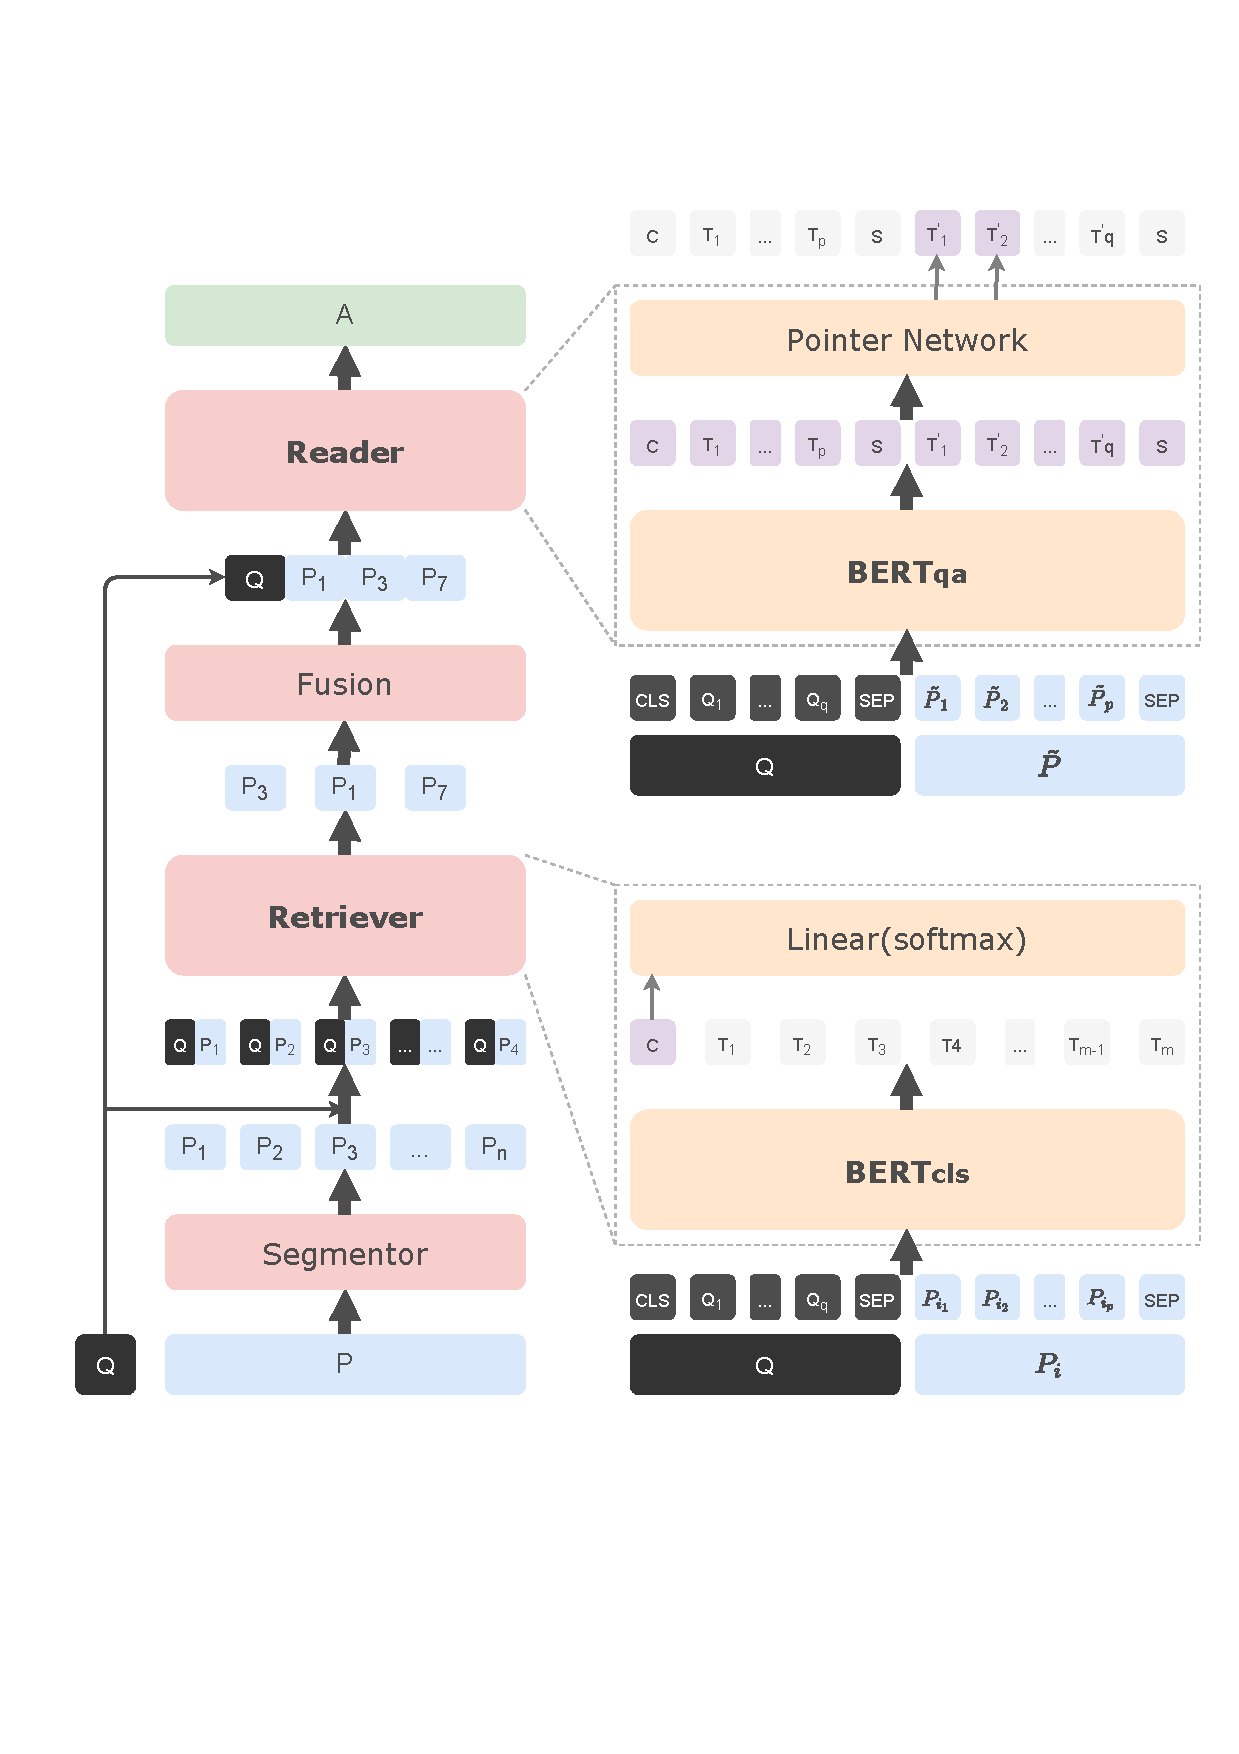
\includegraphics [width=0.8\textwidth] {figure/3-1.pdf}
        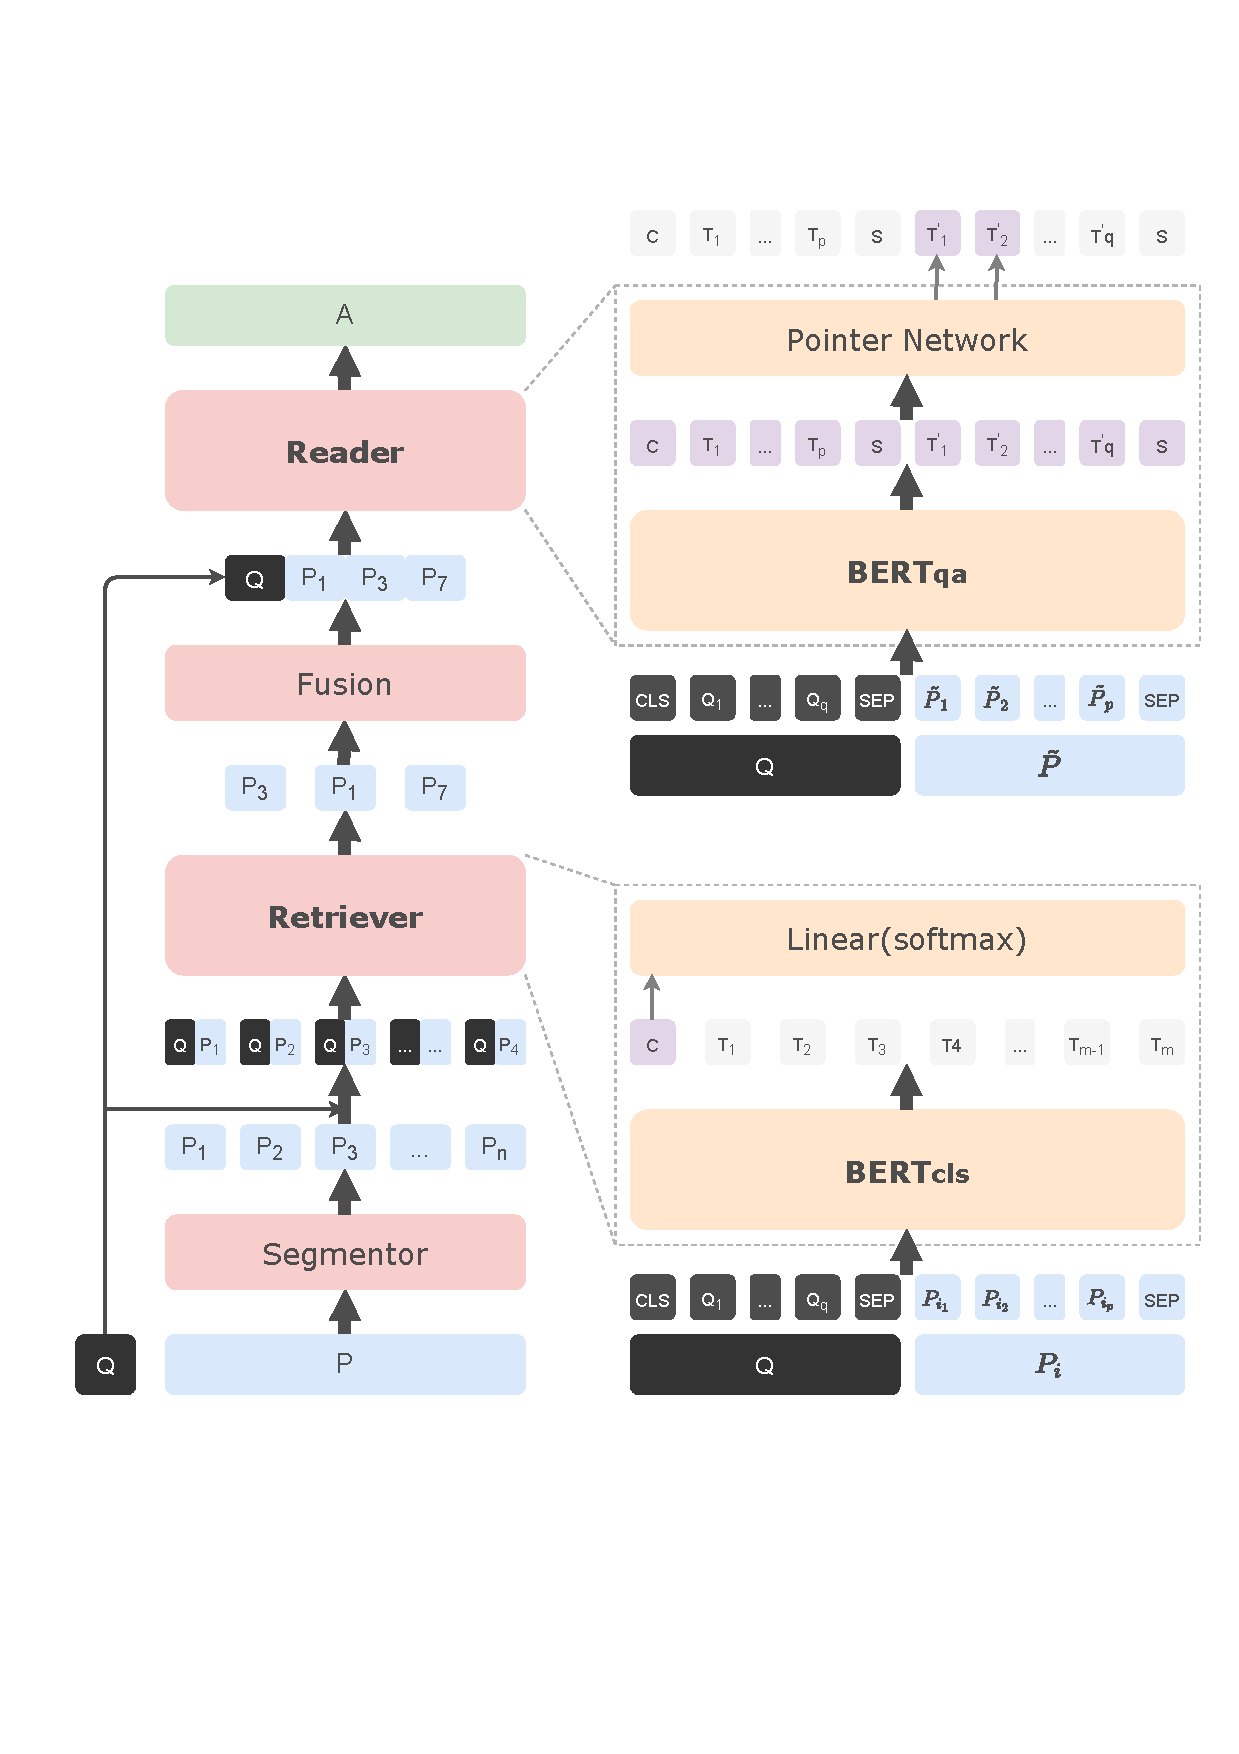
\includegraphics[scale=0.6]{figure/3-1.pdf}
    \caption{ThinkTwice的基本架构}
    \label{fig:3-1}
\end{figure}


\subsection{分段方法}
长文本阅读理解的主要挑战在于如何在给定文章中的大量知识片段中准确地定位到最重要的信息。
这些文章的长度通常超过现有神经网络模型所能容纳的最大长度(例如512个token)。
为了应对这个问题,我们在NewsQA数据集中为每篇文章的结尾添加了一个分割标记。
通过这种方式,可以将输入文本$P$分割成文本片段$P_1,P_2,...,P_n$,其中每个文本片段的长度限制在60-80个token左右。
这种形式化的分割方法可以有效地提高模型的处理效率和准确性。

\subsection{基于预训练语言模型的段落检索器}
当人们需要从大量文本中寻找答案时,通常会选择保留与当前问题最相关的文本片段,并过滤掉琐碎的信息。
受到这种人类行为的启发,本文提出了一个基于预训练语言模型的检索器,来选择最有可能回答问题的最重要的文本片段。

具体而言,检索器部分首先将问题$Q$和每个文本片段$\{P_i\}^n_{i=1}$组合成多个序列$\{x_i\}^n_{i=1}$,其中$x_i=[CLS]Q[SEP]P_i[SEP]$\footnote{[CLS]和[SPE]是特殊token。前者对于编码后的输入序列,理论上可以表示整体信息;后者主要用于分隔输入序列}。
然后,检索器的编码器部分,也就是预训练语言模型,用于将输入$x_i$编码成整个序列的上下文词嵌入表示$H_i$:
\begin{equation}
    H_i = BERT_{cls}(x_i).
\end{equation}

[CLS]的隐向量表示$H^{cls}_i$代表了整个序列的总体表示。
然后,一层线性网络和Softmax层用于得到该序列的分类概率$\hat y_c$:
\begin{equation}
    \hat y_c=Softmax(Linear(H_i^{cls})),
\end{equation}

其中$\hat y_c$表示当前文本片段$P_i$是否包含可以回答给定问题的有效信息\cite{zhang2020retrospective}。
在训练阶段,当$P_i$包含标注答案时,“有/无答案”标签$y_{c(i)}$设为1,否则设为0。

交叉熵损失函数用于计算真实答案$y_c$和预测概率$\hat y_c$之间的损失:
\begin{equation}
    \mathcal  L_{retriever}  = -\frac{1}{n}\sum_{i=1}^{n}[y_{c(i)}\log\hat y_{c(i)}+(1-y_{c(i)})log(1-\hat y_{c(i)})].
\end{equation}

\subsection{融合方法}
上一小节利用检索器得到了输出概率值$\{\hat y_{c(i)}\}^n_{i=1}$,该值可以量化每个文本片段$\{P_i\}^n_{i=1}$回答给定问题$Q$的可能性大小。
接下来,根据$\hat y$的值,选择与问题$Q$最相关的$k$个文本片段,并舍弃其他片段。
被选中的文本片段按照它们在原文中的顺序合并成单个序列,以确保整个组合文本的语义连贯性和上下文连续性。
例如,当$k=3$且分数最高的3个文本片段分别是$P_3$,$P_1$和$P_7$时,融合器需要根据它们在原文中的相对顺序将它们拼接在一起。
对于可能出现的特别长的文本,融合器可以直接对其进行截断。
因此,融合器的输出可以表示为图~\ref{fig:3-1}~中的$\tilde P=<P_1,P_3,P_7>$。

\subsection{基于预训练语言模型的阅读理解模型}
通过以上模块,已经从原始的长文本$P$中提取了一段短文本$\tilde P$。
本节中的阅读器模块首先将问题$Q$和上一节得到的$\tilde P$拼接成一个单独的序列$z=[CLS]Q[SEP]\tilde P[SEP]$,随后使用另一个预训练语言模型BERT\cite{devlin2018bert}作为阅读器的编码器,将输入$z$映射到一个上下文隐向量序列。
下一步,指针网略将问题相关的文本表示的答案片段的起始和结束位置进行解码:
\begin{equation}
    \hat y_s,\hat y_e = PN(BERT_{qa}(z)),
\end{equation}

其中$\hat y_s$和$\hat y_e$分别表示由阅读器解码的预测答案的起始和结束位置的概率。

在训练过程中,阅读器中使用了交叉熵损失来计算起始和结束位置的损失:
\begin{equation}
    \mathcal L_{reader} = \frac{1}{2} CrossEntropy(\hat y_s,y_s) + \frac{1}{2} CrossEntropy(\hat y_e,y_e)
\end{equation}
其中,$y_s$和$y_e$分别表示开始和结束位置的标签。
如果当前段落给出的信息不能回答问题,$y_s$和$y_e$都设为0,也就是指向$[LCS]$token。
在预测阶段,阅读器首先计算“有答案”分数$score_{has}$和“无答案”分数$score_{null}$,各自用$\hat y_s$和$\hat y_e$来表示:
\begin{equation}
    score_{has}=\max \limits_{1\le i\le j<L}(\hat y_{s}^{(i)}+\hat y_{e}^{(j)})
\end{equation}
\begin{equation}
    score_{null}=\hat y_{s}^{(0)}+\hat y_{e}^{(0)}
\end{equation}
其中$i$和$j$表示在整个序列长度$L$内的答案位置,并且由于起始位置一定在结束位置之前,有$i$一定限制为小于$j$。
另外,鉴于序列首部的$[CLS]$不表示$\tilde P$中的任何词,$\hat y^{(0)}_s$和$\hat y^{(0)}_e$表示整个文本没有答案的概率。

接下来,通过计算$score_{has}$和$score_{null}$之间的距离来计算两者之间的距离分数$score_{dist}$,以此作为“有/无答案”的依据:
\begin{equation}
    score_{dist}=score_{null}-score_{has}
\end{equation}
\begin{equation}
    s,e=\argmax \limits_{1\le i\le j<L}(\hat y_{s}^{(i)}+\hat y_{e}^{(j)})
\end{equation}
其中有一个阈值$\delta$,如果$score_{dist}$小于$\delta$,阅读器输出的$s$和$e$就代表了答案的起始和结束位置,否则阅读器会将该问题视为一个不可回答问题。

\section{实验及结果分析}

\subsection{实验设置}
本章在一个具有挑战性的长篇文本阅读理解数据集NewsQA上进行了实验。
该数据集包含来自CNN的13,000篇新闻文章,以及120,000条人工生成的问题答案对。
在排除了20,000条标注者认为没有意义的低质量问题后,本章对剩余的数据进行了实验分析。
因此,NewsQA的训练/开发/测试集分别包含90,000/5,000/5,000条问题答案对。
此外,本章还具体统计了每篇文章的token数量(即tokens per passage, TPP)和每篇文章的段落数量(即paragraphs per passage, PPP)。
在训练/开发/测试集上,TPP的中位数分别为774/734/707,最大值分别为3,100/2,300/2,300。
而PPP在三个集上的中位数为18/18/17,最大值为87/63/54。

针对NewsQA数据集,存在一些长文本模型。
\begin{itemize}
    \item Match-LSTM\cite{wang2015learning}。该模型使用了两个单向的LSTM来编码问题和文章。
    \item BiDAF\cite{seo2016bidirectional}。BIDAF的核心思想是其中的双流注意力层,双流注意力分别计算上下文之于问题的注意力以及问题之于上下文的注意力。
    \item AMANDA\cite{kundu2018question}。AMANDA针对答案抽取提出了一种端到端的专注于问题的多因子注意力网络。多因子注意力编码聚合了位于多个句子中有意义的事实。
    \item DecaProp\cite{tay2018densely}。该模型把自注意力网络整合进RNN模\cite{mikolov2010recurrent}型。
    \item Longformer\cite{beltagy2020longformer}。该预训练语言模型使用了稀疏注意力矩阵,来解决序列长度的限制。
    \item CogLTX\cite{ding2020cogltx}。CogLTX架构通过判别多个句子间的相关性来识别重要句子。
\end{itemize}

本章采用EM和F1这两个官方指标来衡量长文本机器阅读理解的性能。
其中,EM指标用于衡量预测答案与真实答案完全匹配的比例,而F1指标则用于衡量预测答案与真实答案在token级的平均重叠程度。

为了验证两阶段阅读策略的有效性,本章使用了部分预训练语言模型,并采用将文章划分成多个段落的滑动窗口机制来处理长文本阅读理解问题。
所采用的预训练语言模型包括BERT\cite{devlin2018bert}、RoBERTa\cite{liu2019roberta}、ALBERT\cite{lan2019albert}和SpanBERT\cite{joshi2020spanbert},这些模型均基于Transformer\cite{vaswani2017attention}架构,且使用PyTorch实现。
在训练阶段,基础模型的学习率设为2e-5,而大模型的学习率则设为2e-6。此外,热身比例设为0.1,L2权重衰减设为0.01。
批量尺寸在基础模型中为8,在大模型中为1。
对于检索器,轮次数量在基础模型中设为1,在大模型中设为2;
而阅读器中这个值保持为3。
在分词方面,本章采用wordpieces\cite{wu2016google}进行分词,并将第一阶段的最大长度设为256,第二阶段的最大长度设为512。
第一阶段中进行了大量实验,用来选择$k$值\footnote{$k$值是一个超参数,表示检索器筛选出的最好的$k$个段落。}。

\begin{table}[]
    \centering
    \caption{The performances of LT-MRC models on NewsQA as well as our models' performances compared to their corresponding pre-trained language models.}
    \begin{tabular}{p{140pt}p{24pt}<{\centering}p{24pt}<{\centering}p{24pt}<{\centering}p{24pt}<{\centering}}
        %  \thickhline
         \hline
         {\bfseries Model} & \multicolumn{2}{c}{\bfseries Dev} & \multicolumn{2}{c}{\bfseries Test} \\
         & {\bfseries F1} & {\bfseries EM} & {\bfseries F1} & {\bfseries EM} \\
         \hline
         Match-LSTM~\cite{wang2015learning} & 49.6 & 34.4 & 50.0 & 34.9 \\
         BiDAF~\cite{seo2016bidirectional} & - & - & 52.3 & 37.1 \\
         AMANDA~\cite{kundu2018question} & 63.3 & 48.8 & 63.7 & 48.4 \\
         DecaProp~\cite{tay2018densely} & 65.7 & 52.5 & 66.3 & 53.1 \\
         Longformer-base~\cite{beltagy2020longformer} & 68.1 & 58.3 & 68.1 & 58.1 \\
         CogLTX~\cite{ding2020cogltx} & - & - & 70.1 & 55.2 \\
         \hline
         \hline
         BERT-base~\cite{devlin2018bert} & 65.6 & 56.3 & 65.4 & 55.2 \\
         $\ $ + ThinkTwice(descending order) & 66.6 & 57.8 & 65.8 & 55.6 \\
         $\ $ + ThinkTwice(ours) & {\bfseries 68.5} & {\bfseries58.8} & {\bfseries68.6} & {\bfseries57.7} \\
         \hline
         RoBERTa-base~\cite{liu2019roberta} & 63.7 & 53.5 & 63.2 & 53.1 \\
         $\ $ + ThinkTwice(ours) & {\bfseries67.7} & {\bfseries58.6} & {\bfseries67.7} & {\bfseries58.4} \\
         \hline
         ALBERT-base~\cite{lan2019albert} & 68.1 & 58.2 & 68.0 & 58.0 \\
         $\ $ + ThinkTwice(ours) & {\bfseries68.7} & {\bfseries59.1} & {\bfseries68.6} & {\bfseries58.8} \\
         \hline
         SpanBERT-base~\cite{joshi2020spanbert} & 67.7 & 57.1 & 67.5 & 56.2 \\
         $\ $ + ThinkTwice(ours) & {\bfseries69.9} & {\bfseries59.8} & {\bfseries69.7} & {\bfseries59.4} \\
         \hline
         BERT-large & 68.9 & 59.2 & 68.8 & 58.6 \\
         $\ $ + ThinkTwice(ours) & {\bfseries70.1} & {\bfseries59.5} & {\bfseries69.8} & {\bfseries59.4} \\
         \hline
         SpanBERT-large & 71.2 & 61.8 & 70.9 & 59.8 \\
         $\ $ + ThinkTwice(ours) & {\bfseries72.1} & {\bfseries62.2} & {\bfseries71.5} & {\bfseries61.0} \\
        %  \thickhline
         \hline
    \end{tabular}
    \label{tab:3-1}
\end{table}


\subsection{实验结果和分析}
\textbf{与现有模型相比}。
表~\ref{tab:3-1}~呈现了ThinkTwice模型与现有模型的比较结果。
该表说明,本章提出的模型在NewsQA数据集上表现卓越,超越了现有的长文本阅读理解模型。
具体而言,在EM指标上,本模型相比现有模型提升了5.8个百分点,在F1指标上提升了1.4个百分点。
此外,实验结果也同样表明,实现ThinkTwice策略可以提高所有预训练阅读理解模型的性能。
例如,在BERT-base模型上,F1值提高了3.2个百分点,在RoBERTa-base模型上,F1值提高了4.5个百分点。
然而,在ALBERT-base模型上的提升并不显著。
这可能有两个原因:首先,ALBERT模型中的句子顺序预测(sentence-order prediction,SOP)预训练任务已经解决了句子内部连贯性的问题;
其次,ALBERT模型中实现了跨层参数共享机制,导致即使实现了新的策略,参数变化也非常微小。
在其他模型上实验性能的大幅提升表明,ThinkTwice策略中的检索器精准地抽取了最重要的段落,从而将长文本压缩成合适长度的短文本,同时最大程度地保留了原始文本中最重要的信息。

此外,为了研究不同融合方式对最终性能的影响,本章还尝试在BERT-base模型上采用两种不同的融合策略来合并筛选出的文本片段。
其中一种方法是将检索器提取出的文本片段按照与给定问题的相关性进行降序排列并进行合并;
另一种方法是按照先前所述的方法,以原文的顺序进行合并。
从表格~\ref{tab:3-1}~中的第8行和第9行可以发现,原始的融合方式要显著优于降序的融合方式(提升2.8),尽管采用降序方式排列的模型也超出了基线模型(0.4)。
这个对比实验表明,扰乱序列顺序可能会导致上下文信息的丢失。

\begin{figure}[htbp]
    \centering
    % 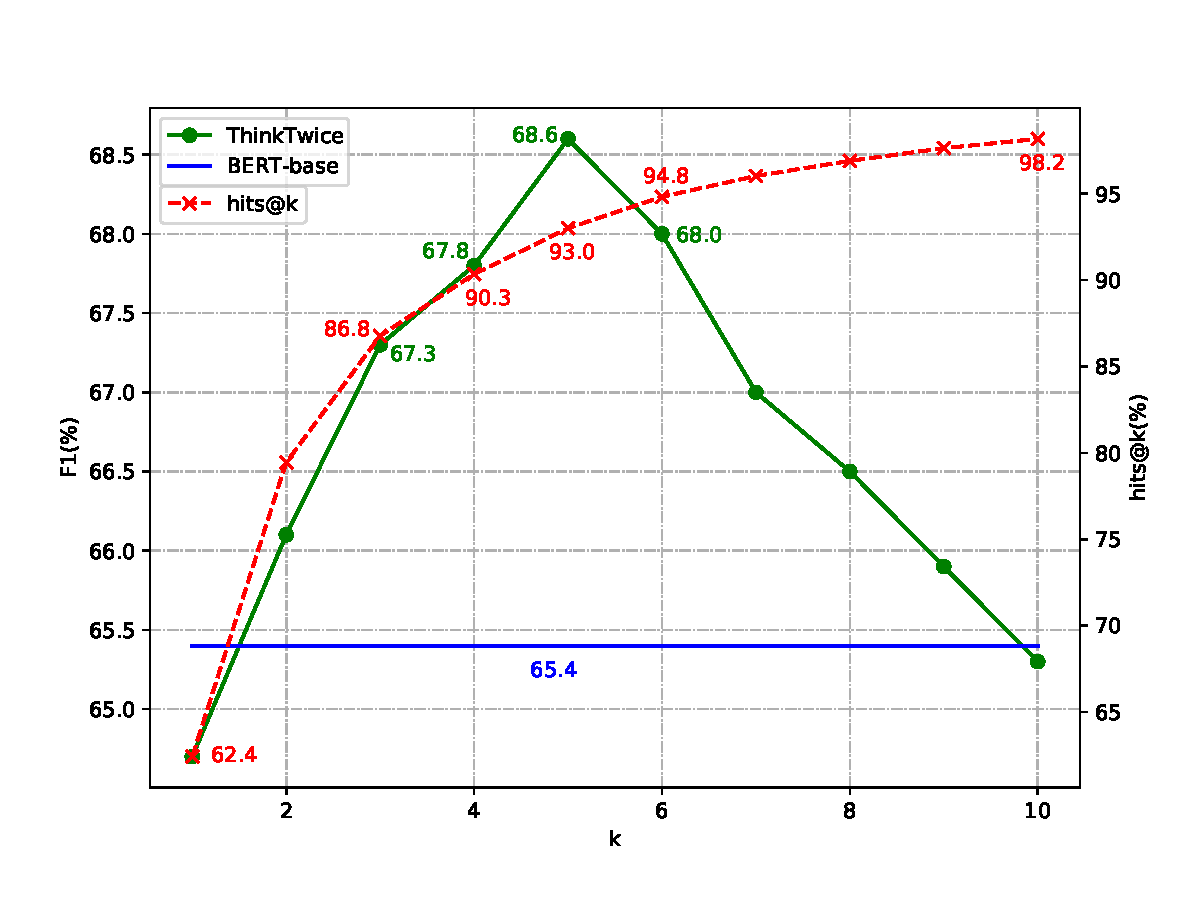
\includegraphics[width=\textwidth]{figure/3-2.pdf}
    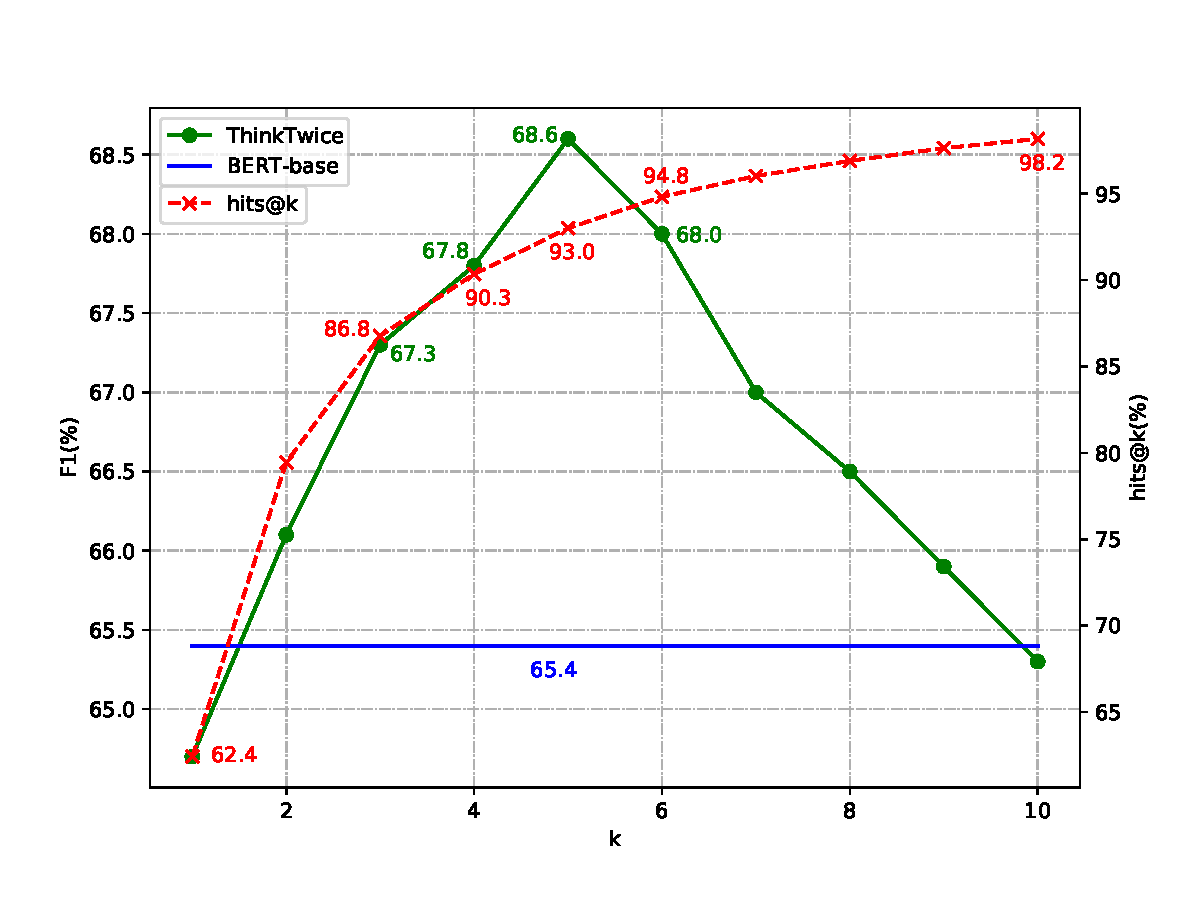
\includegraphics[scale=0.7]{figure/3-2.pdf}
    \caption{在不同$k$值情况下,检索器和ThinkTwice模型(基于BERT-base)的性能关联}
    \label{fig:3-2}
\end{figure}

\begin{figure}
    \centering
    % 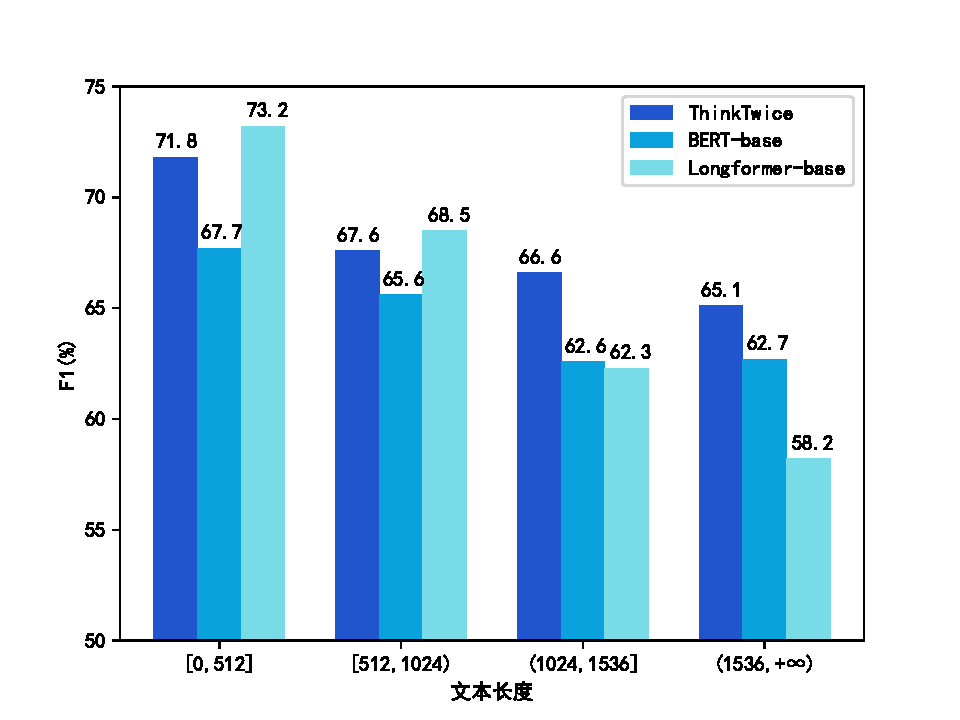
\includegraphics[width=0.7\textwidth]{figure/3-3.pdf}
    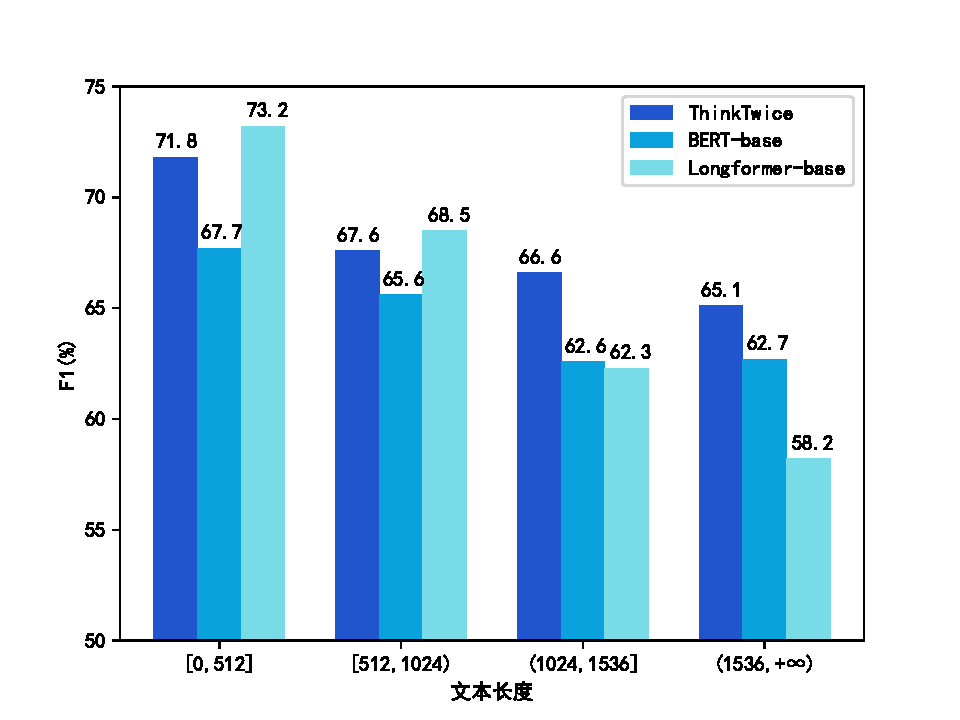
\includegraphics[scale=0.7]{figure/3-3.pdf}
    \caption{Performances of ThinkTwice, BERT-base, and Longformer-base over different text lengths. The number of samples in the four length intervals are: 1,611, 2,074, 1,089, and 210.}
    \label{fig:3-3}
\end{figure}


\textbf{段落检索}。
图~\ref{fig:3-2}~展示了检索器的不同参数配置与ThinkTwice模型之间的关系。
对于检索器,评估指标Hits@$k$(前$k$个最准确的)衡量了检索器筛选出的最佳$k$个段落是否包含真实答案。
对于ThinkTwice模型,F1评估NewsQA数据集上阅读理解模型的最终性能。
红色曲线表明,$k$值越大,Hits@$k$准确率就越高。同时,当$k$大于3时,检索器的该项指标也超过了90\%。
此外,当$k$等于5时,ThinkTwice模型(绿色曲线)实现了最佳性能(68.6)。
这表明,当$k$值较小时,检索器无法召回足够多的备选段落;
当$k$大于5时,更多的备选段落需要搜索更大的文本范围,从而导致性能下降。
因此,ThinkTwice在所有实验中将超参数$k$设为5。
本节还将ThinkTwice模型与相应的BERT-base阅读理解模型(蓝色曲线)进行了比较。
结果显示,当$k$设为2到9之间时,ThinkTwice模型的表现优于BERT-base,这验证了ThinkTwice两阶段策略的有效性。

\textbf{文本长度的作用}。
为了验证ThinkTwice在长文本领域的作用,本节将对多个不同长度的文本进行测试,并将测试结果与BERT-base和Longformer-base等阅读理解模型进行比较。
值得注意的是,这里ThinkTwice模型的阅读器应用了BERT-base。
图~\ref{fig:3-3}~列出了实验结果。
可以看到,在较短的文本长度范围内([0,512]和(512,1024]),Longformer实现了最好的实验结果。
其中的原因是Longformer-base继承了RoBERTa的预训练参数权重,而这些参数已经在阅读理解任务中表现得很好。
然而,在较长的文档长度范围内((1024,1536],(1536,$+\infty$)),本章提出的ThinkTwice模型显著优于其他模型。
这也证实了ThinkTwice能够准确地定位到包含答案的文本片段。
此外,在较长文档的实验结果中,BERT-base也要优于Longformer-base,这表明滑动窗口机制(BERT-base)相较于直接的长文本输入(Longformer-base),也有一定优势。
最后可以发现,随着文档长度的增加,ThinkTwice模型的性能是最稳定的,特别是当文本长度大于512的时候。

\begin{table}[htbp]\scriptsize
    \centering
    \caption{NewsQA数据集上两个关于三个基线模型和CoLISA模型的预测的例子}
    \begin{tabular}{p{408pt}}
        \hline
        \multicolumn{1}{c}{\bfseries 例子1} \\
        \hline
        文章:\\
        (CNN) -- President Barack Obama spoke with Egypt's president moments after Hosni Mubarak addressed his country, telling the Egyptian that \textcolor[rgb]{1,0,0.2}{he must make good on his promises} and avoid a violent response to the thousands of protesters in the streets. (...) \\
        <译文:(...) 巴拉克·奥巴马总统在穆巴拉克发表讲话后不久与埃及总统进行了交谈,告诉埃及总统他必须履行承诺,避免对街头上万名抗议者采取暴力行动。(...) > \\
        \hline
        Token数量:2,036 \\
        \hline
        问题:\\
        What did Obama say to Mubarak? \\
        <译文:奥巴马对穆巴拉克说了什么?> \\
        \hline
        答案:\\
        he must make good on his promises \\
        <译文:他必须遵守诺言> \\
        \hline
        CoLISA预测:\\
        \textcolor[rgb]{1,0,0.2}{he must make good on his promises and avoid a violent response} (True) \\
        <译文:他必须遵守诺言并避免采取暴力行动> \\
        \hline
        BERT预测:\\
        I just spoke to him after his speech (False)
        <译文:我在他演讲结束以后跟他讲过> \\
        \hline
        ALBERT预测:\\
        It is very important that people have mechanisms in order (False) \\
        <译文:人们拥有机制非常重要> \\
        \hline
        Longformer预测:\\
        he must make good on his promises and avoid a violent response (True) \\
        <译文:他必须遵守诺言并避免采取暴力行动> \\
        \hline
        % \hline
        \multicolumn{1}{c}{\bfseries 例子2} \\
        \hline
        文章:\\
        (...) Tucked away in the verdant hills west of St. Andrews, Kingarrock Hickory Golf Course (greens fee, \$40 for nine holes and \$55 for 18) \textcolor[rgb]{1,0,0.2}{is a nine-hole, 2,022-yard country estate course that is played exclusively with antiquated equipment}. (...) \\
        <译文:(...) 坐落在圣安德鲁斯西部郁郁葱葱的山丘上,Kingarrock Hickory高尔夫球场(九洞的场地费为40美元,18洞的场地费为55美元)是一个九洞、2022码的乡村庄园球场,球场上全部使用古董设备打球。(...) > \\
        \hline
        Token数量:2,288 \\
        \hline
        问题:\\
        What is Kingarrock Hickory? \\
        <译文:Kingarrock Hickory是什么?> \\
        \hline
        答案:\\
        is a nine-hole, 2,022-yard country estate course that is played exclusively with antiquated equipment \\
        <译文:是一个九洞、2022码的乡村庄园球场,球场上全部使用古董设备打球> \\
        \hline
        CoLISA预测:\\
        \textcolor[rgb]{1,0,0.2}{a nine-hole, 2,022-yard country estate course that is played exclusively with antiquated equipment} (True) \\
        % CoLISA预测:\underline{a nine-hole, 2,022-yard country estate course that is played exclusively with antiquated equipment (True)} \\
        <译文:一个九洞、2022码的乡村庄园球场,球场上全部使用古董设备打球> \\
        \hline
        %  BERT预测:\textcolor[rgb]{0.4,0.7,0.9}{the kind of place that can change the way one thinks about golf (False)} \\
        BERT预测:\\
        the kind of place that can change the way one thinks about golf (False) \\
        <译文:一种可以改变人们对高尔夫球看法的地方> \\
        \hline
        ALBERT预测:\\
        Golf Course (True)
        <译文:高尔夫球场> \\
        \hline
        Longformer预测: \\
        Top hotel penthouses (False)
        <译文:顶级酒店顶层套房> \\
        \hline
    \end{tabular}
    \label{tab:3-2}
\end{table}


本章节还进行了一个案例分析,以进一步比较NewsQA上ThinkTwice模型的预测结果与其他模型之间的差异。
研究结果表明,ThinkTwice模型的预测答案与真实答案更加接近。

为了验证模型在处理特别长的文本上的性能,本章节选取了两篇长度超过2,000词的文章作为样例,如表~\ref{tab:3-2}~所示。
在例子1中,模型需要回答奥巴马说了什么,ThinkTwice准确地定位到包含最终答案的第一段段落,并给出了奥巴马说出的合适内容。
然而,BERT和ALBERT却没有像预期那样表现出色,它们分别抽取了其他段落的句子。
在例子2中,ThinkTwice模型同样准确地定位到了正确的段落,而BERT和Longformer的表现则不尽如人意。


\section{本章小结}
本章提出了一种二阶段方法,用于在长文本阅读理解任务中解决预训练语言模型中的长度限制问题。
ThinkTwice模型通过将长文本压缩为较短的文本形式,并准确定位答案位置来实现这一目标。
实验结果和分析表明,该方法在长文本任务上具有有效性。
然而,该方法存在一个潜在的缺陷,即由检索器压缩得到的短文本可能因缺乏先行词而导致不连贯。
因此,未来的研究将集中于通过指代消解或位置词嵌入等方式来解决这个问题。



\chapter{基于对比学习的多项选择长文本阅读理解}
多项选择阅读理解是一种通过阅读并理解一篇给定文章和问题,从多个备选答案中选出最合适答案的任务。
近期的研究致力于捕获文章、问题和选项三元组之间的联系,但由于文本长度过长,模型难以重点关注备选答案之间的联系,导致在面临复杂的多项选择问题时,最近的方法往往会将干扰选项误判为正确答案。
为了解决这一问题,本章提出了一种基于对比学习和样本内注意力的模型CoLISA(Contrastive Learning and In-Sample Attention),该模型通过对比学习和样本内注意力机制,相对精准地剔除干扰选项。
特别地,CoLISA采用对比学习来获取蕴含其他选项信息的选项表示,并应用样本内注意力机制,使得多个选项之间产生联系。
实验结果表明,CoLISA在正确与错误选项之间的联系花费了更多注意力,能够识别选项之间的差异,并在QuALITY数据集上实现了SOTA(state-of-the-art)的性能。


\section{引言}
机器阅读理解(Machine Reading Comprehension, MRC)是一种通过对给定文档进行推理,要求模型回答指定问题的任务。
作为MRC任务的一种变体,多项选择阅读理解(Multi-choice Reading Comprehension, MC-RC)主要针对在给定文章的情况下,从多个备选答案中选出最合适的答案来回答问题。
MC-RC要求模型在阅读并理解参考文章的前提下,判断每个备选答案的正确性。

在MC-RC领域,现有的研究通常集中于解决文章和备选答案之间的差异问题,以解决给定问题\cite{ran2019option,zhang2020dcmn+}。
这些模型通常会对每个选项进行独立编码。
然而,这种方法会限制模型的推理能力,因为对于某个问题,每个选项并不能直观地与其他选项进行交互。
此外,在某些真实情况下,某些备选答案在字面上或语义上与正确答案非常相似,这使得仅仅判断单个选项的正确性变得更加困难。
目前已有的方法往往无法处理这些情况。
因此,本章认为需要采用更精细的方法来处理这些所谓的干扰项与正确答案之间的关系。
表~\ref{tab:4-1}~具体描述了QuALITY\cite{pang2021quality}中一个关于难以辨别的干扰项的实例\footnote{QuALITY中也存在输入文章长度超过模型限制的情况,本章也会在后续讨论这个问题。}。
参考例子中的整篇文章,可以认为正确答案$O_2$(表中红色部分)和干扰选项$O_1$(表中蓝色部分)可以认定都是接近于正确答案的。
为了根据给定问题选出最合适的答案,模型需要找到正确答案和干扰选项表示之间的差异。

\begin{table}[htbp]
    \centering
    \begin{tabular}{p{420pt}}
    \hline
    {\bfseries 文章:} \\
    (...) I'm sure that `justifiable yearnings for territorial self-realization' would be more appropriate to the situation (...) (Over 4,000 words) \\
    <译文:(...) 我确信“对领土自我实现的正当渴望”可能更适用于这种情况 (...) > \\
    \hline
    {\bfseries 问题:} \\
    According to Retief what would happen if the Corps did not get involved in the dispute between the Boyars and the Aga Kagans? \\
    <译文:如果Corps不介入Boyars和Aga Kagans的争端,根据Retief的说法会发生什么? > \\
    \hline
    {\bfseries 选项:} \\
    $O_1$: \textcolor[rgb]{0.4,0.7,0.9}{The Aga Kagans would enslave the Boyars} \\
    <译文:Aga Kagans会奴役Boyars> \\
    $O_2$: \textcolor[rgb]{1,0.4,0.3}{The Boyars and the Aga Kagans would go to war} \\
    <译文:Boyars和Aga Kagans会引发战争 > \\
    $O_3$: The Aga Kagans would leave Flamme to find a better planet \\
    <译文:Aga Kagans会离开Flamme,找到更好的星球> \\
    \textbf{$O_4$}: The Boyars would create a treaty with the Aga Kagans without the Corps' approval \\
    <译文:Boyars会与Aga Kagans签订条约,而不需要得到Corps的批准> \\
    \hline
    \end{tabular}
    \caption{\label{tab:4-1}
    QuALITY中的例子。
    }
\end{table}


人类总是需要通过仔细比较各个选项之间的差异,来排除看上去正确的错误选项,从而回答阅读理解-多项选择问题(MC-RC问题)\cite{daniel2017thinking}。
受到该流程的启发,本章提出了一个基于对比学习和样本内注意力(CoLISA)的架构,它包含两个主要的特点。
首先,由于应用了两次不同的dropout掩码,得到两个有着轻微差异的表示。
也就是说,对于同一个输入,会有两组输出值,每一组都包含了一个正确答案和若干个错误选项。
CoLISA主要通过对比学习的方式,将两个正确选项的表示拉近,然后把正确答案与干扰选项之间的表示推远;
因此,该模型可以学习到更有效的文本表示。
此外,自注意力机制\cite{vaswani2017attention}也应用在了特定样本中的多个选项之间,在选项之间共享彼此的信息。
因此,模型借助多个备选答案之间的自注意力交互的方式,学习到了倾向于选择正确答案的能力。
本章还在两个MC-RC数据集QuALITY\cite{pang2021quality}和RACE\cite{lai2017race}上进行了实验。
实验结果表明,CoLISA的性能表现显著超过其他现有方法。

本章的研究贡献可以概括如下:
\begin{itemize}
    \item[$\bullet$] 引入对比学习方法,以区分多项选择长文本阅读理解任务中正确答案和干扰选项之间的差异。该方法通过赋予干扰选项更多的权重,从而使其获得更多的注意力。
    \item[$\bullet$] 针对一个特定的例子,将样本内注意力机制应用于多个选项之间,促进它们之间的互动。
    \item[$\bullet$] 本章提出的CoLISA方法在QuALITY上实现了SOTA的性能,并在RACE上相对于其他基线模型实现了显著的提升。
\end{itemize}


\section{基于对比学习的多项选择长文本阅读理解}
给定一篇参考文本,一个目标问题,还有一些备选答案,多项选择阅读理解(multi-choice reading comprehension, MC-RC)任务是指将其中一个选项预测为最终答案。
形式上来说,将一篇文章定义为$p=[s^p_1, s^p_2, ..., s^p_n]$,其中$s^p_i=[w^s_1, w^s_2, ..., w^s_l]$表示$p$中第$i$个句子,$w^s_j$表示$s^p_i$中的第$j$个词。
问题可以定义为$q=[w^q_1, w^q_2, ..., w^q_t]$,其中$w^q_i$表示$q$中的第$i$个词。
选项集合可以定义为$O=[o_1, o_2, ..., o_r]$,其中$o_i=[w^o_1, w^o_2, ..., w^o_k]$表示第$i$个选项,$w^o_k$表示$o_i$中第$k$个词。
MC-RC的目标是最大化所预测选项的概率:
\begin{equation}
    a = \argmax_i(\mathcal P(o_i|p,q))
\end{equation}

当$p$的长度超过编码器的最大输入长度时,本章的做法是通过检索与问题和备选答案相关的句子,将长文本压缩成篇幅较短的文本。
较短文本表示为$c=[s^c_1, s^c_2, ..., s^c_m]$,其中$s^c_i=[w^s_1, w^s_2, ..., w^s_l]$表示$c$中的第$i$个句子,$w^s_j$表示$s^c_i$中的第$i$个句子。

\subsection{总体架构}
如图~\ref{fig:4-1}~所示,本章提出了一种新颖的MC-RC框架,它充分运用了对比学习和样本内注意力(Contrastive Learning and In-Sample Attention, CoLISA),主要由两部分组成:
首先是基于DPR(Dense Passage Retrieval,稠密检索)的检索器,在一篇很长的文章中,根据对给定问题和对应的过个备选答案之间的相关性,筛选出相关的句子,以此来根据原文的原始顺序来构建一段新的文本;
另外,CoLISA阅读器需要根据给定问题和上下文中,从若干选答案中预测出最终答案。
CoLISA阅读器由两部分组成。
第一部分是样本内注意力(In-Sample Attention, ISA)机制,换句话说,引入一个加入了多头自注意力机制并针对长序列的网络,来增强特定样本中多个选项之间的交互。
第二部分是对比学习(Contrastive Learning,CoL)以及一个干扰因子(Distractive Factor,DiF),来表示由上下文、问题和备选答案组合而成的序列。

% 模型图
\begin{figure}[htbp]
    \centering
    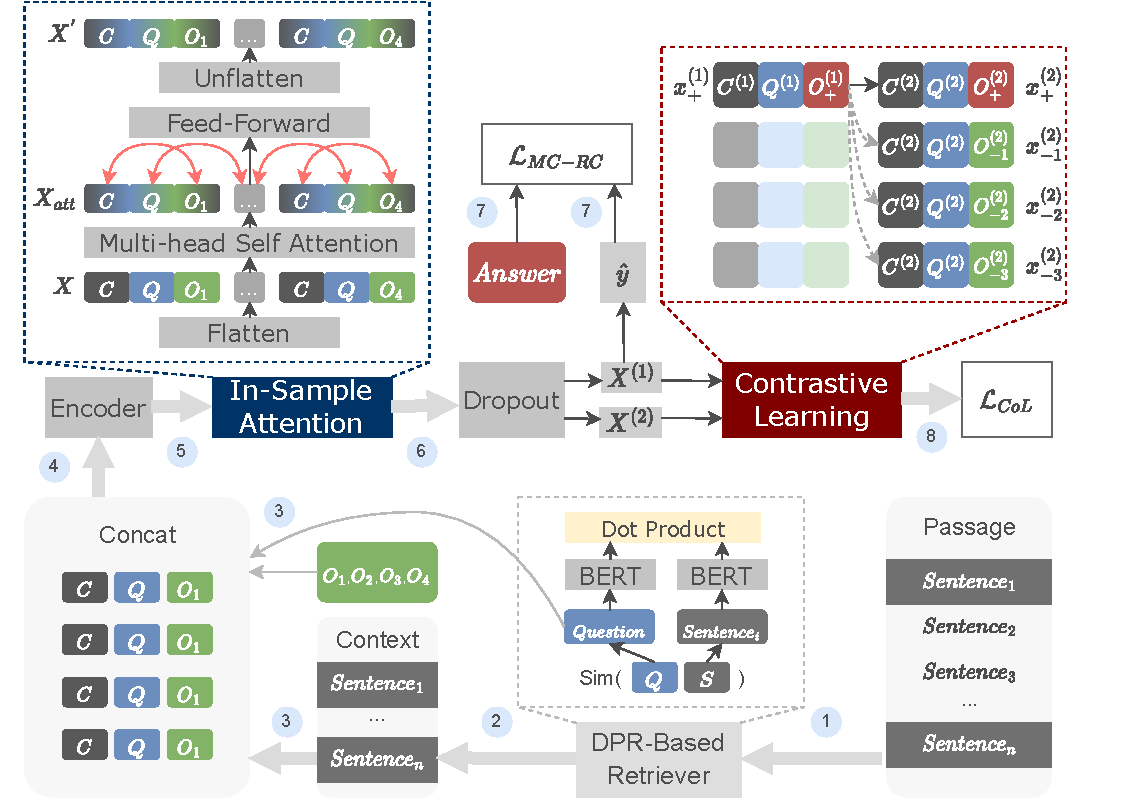
\includegraphics [width=1.0\textwidth] {figure/4-1.pdf}
    % \caption{The architecture of our model CoLISA. (1) A long passage is fed into the DPR-based retriever, (2) then comes out a shorter context, (3) together with a related question and multiple options in our dataset, they are (4) preprocessed and combined into four different sequences (in our dataset there are four options for each question), after going through the inherent (5) embedding and (6) encoder, these four sequences are represented as (7) vector representations, (8) followed by an ISA module listed on the right top of the figure, the sequences are flattened to a combined one, with multi-head self-attention across each token within the extended sequence, then the sequence roll back to the initial dimension, (9) the updated vectors are fed into a dropout twice to come out into two outputs, (10) one for calculating the cross-entropy loss (11) meanwhile both of them need feeding to a CoL module illustrated on the left top of the figure, to calculate a contrastive learning loss finally.}
    \caption{CoLISA的基本架构。} % Our proposed contrastive learning method and in-sample attention mechanism are highlighted boldly in dark red and dark blue rectangles, respectively.
    \label{fig:4-1}
\end{figure}


\subsection{基于DPR的检索器}
为了从一篇长文本中筛选出相关的句子,本节首先采用基于DRP(Dense Passage Retrieval,稠密检索)的句子检索器。
该检索器常用于隐式语义编码\cite{karpukhin2020dense}。
值得注意的是,DPR提供了两个不同的编码器,用于预训练抽取不同种类的句子,本节使用相应的DPR编码器以确保检索到的句子具有多样性。
上下文编码器$E_S$将参考文章$p$中的所有句子$s$编码为$d$维向量。
类似地,查询编码器$E_R$将问题$q$和选项集合$O$编码为$d$维向量,作为两种不同的检索查询$r$。
$s$和$r$的$[CLS]$token的全局表示用于计算它们的负欧几里得距离($L^2$):
\begin{equation}
    -L^2_{dist}(r,s)=-||E_R(r)-E_S(s)||^2
\end{equation}

针对选项查询,本节按照$s$和$r$之间的相关性降序排列,选择前$k$个句子,并考虑到语义连贯性的问题,筛选出这$k$个句子的前一句和后一句。
然而,同一个句子可能会被多次选择,因此需要去重。
最终得到$k$个唯一的句子作为参考上下文。

对于问题查询,首先选择前$n$个句子作为参考上下文\footnote{考虑到预训练语言模型能容纳所抽取的句子的总长度,$k$和$n$需要设定为合适的值,这里在所有实验中将$k$设为2,$n$设为1。}。
由于来源于选项的证据相比于来源于问题的证据更合适,所以本节不采集前一句和后一句。
同样,需要通过去重来确保所有抽取句子的唯一性。

在选出最合适的句子后,再根据原文顺序将这些句子进行排序,然后将它们拼接成一段参考上下文$c$。
算法~\ref{alg:4-2}~详细阐述了抽取的过程。

% \begin{algorithm}\small
%   \KwIn{Passage $p=[s_1, s_2, ..., s_n]$, Question $q$, Options $O=[o_1, o_2, ..., o_m]$}
%   \KwOut{Context}
%   \eIf{Input (x) belongs to p}{
%     $E_x$ = ContextEncoder($x$)\;
%     }{
%     $E_x$ = QuestionEncoder($x$)\;
%     % $E_o$ = QuestionEncoder($o$)\;
%     }
%   \For{$o_i$ in $O$}{
%     \For{$s_j$ in $p$}{
%       sim($o_i$, $s_j$) = -L^2_{dist}($E_{o_i}$, $E_{s_j}$)
%       }
%     Select: Top-k relevant sentences $s_{i_1}, s_{i_2}, ..., s_{i_k}$\;
% 	Select: Their previous and next sentences $s_{i_1}^{prev}, s_{i_1}^{next}, ..., s_{i_k}^{prev}, s_{i_k}^{next}$\;
% 	Context $\gets$ Selected sentences\;
% 	}
%   \For{$s_j$ in $p$}{
%     sim($q$, $s_j$) = -L^2_{dist}($E_q$, $E_{s_j}$)
% 	}
%   Select: Top-n relevant sentences $s_{j_1}, s_{j_2}, ..., s_{j_n}$\;
%   Context $\gets$ Selected sentences\;
%   Context.unique().sort().to\_str()\;
%   \caption{\label{alg:algorithm}The Extracting Algorithm}
% \end{algorithm}


\begin{algorithm}\small
  % \KwIn{Passage $p=[s_1, s_2, ..., s_n]$, Question $q$, Options $O=[o_1, o_2, ..., o_m]$}
  % \KwOut{Context}
  % \eIf{Input (x) belongs to p}{
  %   $E_x$ = ContextEncoder($x$)\;
  %   }{
  %   $E_x$ = QuestionEncoder($x$)\;
  %   % $E_o$ = QuestionEncoder($o$)\;
  %   }
  % \For{$o_i$ in $O$}{
  %   \For{$s_j$ in $p$}{
  %     sim($o_i$, $s_j$) = -L^2_{dist}($E_{o_i}$, $E_{s_j}$)
  %     }
  %   Select: Top-k relevant sentences $s_{i_1}, s_{i_2}, ..., s_{i_k}$\;
	% Select: Their previous and next sentences $s_{i_1}^{prev}, s_{i_1}^{next}, ..., s_{i_k}^{prev}, s_{i_k}^{next}$\;
	% Context $\gets$ Selected sentences\;
	% }
  % \For{$s_j$ in $p$}{
  %   sim($q$, $s_j$) = -L^2_{dist}($E_q$, $E_{s_j}$)
	% }
  % Select: Top-n relevant sentences $s_{j_1}, s_{j_2}, ..., s_{j_n}$\;
  % Context $\gets$ Selected sentences\;
  % Context.unique().sort().to\_str()\;
  \caption{\label{alg:algorithm}The Extracting Algorithm}
\end{algorithm}


\subsection{样本内的自注意力机制}
在进行编码$q$和$o_i$时,针对同一个问题,每个备选答案的编码都是相互独立的,这导致在计算注意力时可能会出现注意力缺失的问题。
为了解决这个问题,本章借鉴了人类回答多项选择问题的方式,即通过同时比较多个选项来排除干扰项,最终决定选择哪个选项。
基于这种思路,本章提出了一种样本内注意力(In-Sample Attention)机制,以增强不同选项表示之间的交互作用。

通常,每个备选答案$o_i$先和它对应的上下文$c$以及问题$q$进行拼接,构成一个三元组$x_i=[c;q;o_i]$。
本章通过将每个$x_i$依次喂入预训练编码器中,从而得到一系列完整的序列表示。
为了建模多个选项$o_i$之间的联系,本章提出的ISA模块首先收集到所有与相同问题$q$对应的$x_i$,对它们进行拼接,构建一个单独的序列$X=[x_1;x_2;...;x_n]$。
然后,计算$X$的自注意力表示,来学习多个选项之间的远程依赖。
具体来说,利用平凡的自注意力机制的架构,同时将序列$X$分解为三个矩阵$Q$,$K$,$V$。
输出的自注意力矩阵可以计算为:
\begin{equation}
    SA(Q,K,V)=softmax(\frac {QK^T}{\sqrt{d_k}})V
\end{equation}
其中$d_k$是一个缩放因子,它表示$K$的维度,以防引起梯度消失现象\cite{vaswani2017attention}。
更进一步,多头注意力机制被引入到ISA中,从不同的向量维度来更加综合性的表示$X$。
多头自注意力的流程可以定义为:
\begin{align}
    & head_i = SA(QW^Q_i,KW^K_i,VW^V_i) \\
    & H = Concat(head_1,...,head_h) \\
    & MSA(Q,K,V) = HW^O
\end{align}
其中$h$表示各个平行注意力头的数量,$W^Q_i,W^K_i,W^V_i,W^O$是注意力参数矩阵。
这里还将多头自注意力的向量表示记为$X_{att}$。
如图~\ref{fig:4-1}~中的ISA机制所描述的,作用在拼接后的序列$X$的注意力机制通过计算选项之间的表示$X_{att}$,实现彼此之间的交互。

此外,为了避免多头自注意力输出的塌陷\cite{vaswani2017attention,sukhbaatar2019augmenting},多头自注意力机制后面还增加了一个全连接网络:
\begin{equation}
    X_{ffn}=FFN(X_{att})
\end{equation}
这里使用了GeLU\cite{hendrycks2016gaussian}函数作为激活函数。
最终,$X_{fnn}$需要根据多个输入三元组$x_i$的维度拆解为多个表示。
输出三元组的结合记为$X^{'}$。

\subsection{面向备选答案交互的对比学习方法}
为了推动CoLISA在明确区分正确答案和干扰选项表示之间的差异方面的表现,本节引入了对比学习(Contrastive Learning,CoL)模块。
受通用对比学习框架\cite{gao2021simcse}的启发,CoL模块旨在通过将同一样本内的所有表示均匀分布在特定的向量空间上,促进两个正向三元组表示之间的变得更加接近。

在上一节介绍的ISA模块之后,具有交互注意力的输入向量$X^{'}$通过dropout层进行传递,并进行两次相同的操作,以针对每个输入生成两个略有差异的编码表示,分别记为$X^{(1)}$和$X^{(2)}$。

之后,先要计算MC-RC任务中在目标标签$y$和输出$X^{(1)}$之间的交叉熵损失。
具体来说,通过一层全连接神经网络可以将$X^{(1)}$转换为预测输出$\hat y$,它的维度与标签$y$相同。
损失函数定义如下:
\begin{equation}
    \begin{split}
    \mathcal L_{MC-RC}=& -\frac{1}{N}\Sigma^N_{i=1}(y^{(i)}\log\hat y^{(i)}+(1-y^{(i)})\log(1-\hat y^{(i)}))
    \end{split}
\end{equation}
注意到来自同一样本的输出$X^{(1)}$和$X^{(2)}$均由相同数量的三元组$x_i$组成,其中包含一个正确答案的三元组以及其余包含错误答案的三元组。
因此,对于每个输入样本的两个输出结果,对比损失可以被定义为负对数似然函数的平均值。
具体而言,对于其中一个输出$X^{(1)}$,本节将包含正确答案的三元组作为锚点,并移除包含错误选项的三元组。
对于另一个输出$X^{(2)}$,所有三元组均被保留,其中包含正确选项的三元组视为正例,而其他三元组则被视为负例。
每个损失项均能够区分正例和负例之间的差异。

CoL的损失函数定义如下:
\begin{equation}
    \mathcal L_{CoL}=-\frac{1}{N}\Sigma^N_{j=1}\log \frac{e^{sim(x^{(1)}_+,x^{(2)}_+)/ \tau}}{\Sigma^S_{i=1} e^{sim(x^{(1)}_+,x^{(2)}_i)/ \tau}}
\end{equation}
其中$x^{(1)}_+$是$X^{(1)}$中包含正确答案的三元组的编码表示,而$x^{(2)}_i$是$X^{(2)}$中所有三元组的表示,$X^{(2)}$中的$x^{(2)}_+$是正例样本,$\tau$是可配置的超参数,温度系数。
$sim(\cdot)$是一种相似度指标(本章中所有的实验都是使用余弦相似度函数),$S$代表了每个样本中三元组的数目,$N$代表了batch的大小。
聚合后的对比损失$\mathcal L_{CoL}$主要通过在每个batch中的所有样本取平均获得。

\textbf{干扰因子。}
基于样本中不同的干扰项会对模型造成不同程度的干扰,本节还将一个对比因子(Distractive Factor, DiF)引入到了CoLISA模型,具体来说,将DiF结合到对比学习的过程当中。
QuALITY的数据标注人员针对每个问题的所有错误选项中,把误导他们最严重的的那个标记为强干扰项。
因此,本节中通过构建一组置信因子,根据每个选项对应的标注分数,来代表它们对$\mathcal L_{CoL}$的贡献度。
本节中枚举了对每个选项的标注票数来构建DiF $\Theta=[\theta_1, \theta_2, ..., \theta_n]$,其中$n$是备选答案的数量。
然后再用一个softmax函数来帮助缩放$\Theta$,从而更明显的区分每个$\theta_i$。
每个$\theta_i$被修正为如下的形式:
\begin{equation}
    \theta_i=\frac{e^{\theta_i}}{\Sigma^n_i e^{\theta_i}}
\end{equation}
幂运算可以清晰的却分$n$个系数$\theta_i$。
当计算对比损失的时候,$\theta_i$乘上了它对应选项的相似度的值,来衡量正确答案和干扰答案的差距。
$\theta_i$的值越大,对对应选项贡献的损失就越多。
经过上述分析,对比损失函数可以改进为如下:
\begin{equation}
    \mathcal L_{CoL}=-\frac{1}{N}\Sigma^N_{j=1}log \frac{\theta_+e^{sim(x^{(1)}_+,x^{(2)}_+)/ \tau}}{\Sigma^S_{i=1} \theta_ie^{sim(x^{(1)}_+,x^{(2)}_i)/ \tau}}
\end{equation}
其中$\theta_+$和$\theta_i$分别对应样本中的正例以及第$i$个选项。
最终的损失函数可以表示为:
\begin{equation}
    \mathcal L=\alpha \cdot \mathcal L_{MC-RC}+(1-\alpha) \cdot \mathcal L_{CoL}
\end{equation}
其中$\alpha \in[0,1]$是一个平衡系数。


\section{实验及结果分析}
本节首先详细描述了实验的设置,并在此基础上呈现了实验结果。
接着,本节对实验结果进行了进一步的对比和分析,特别是与其他现有模型进行了比较。
此外,本节还进行了一系列消融实验,以验证CoLISA模型的有效性和鲁棒性。

\subsection{实验设置}
本节采用了基准数据集QuALITY和RACE,以评估CoLISA模型的效果。
其中,主要实验是在QuALITY数据集上进行的\footnote{基于DPR的检索器在QuALITY数据集中对于长文本输入的检索是可行的。此外,最强干扰项仅在QuALITY数据集中有标注,因此,大部分实验均在该数据集上完成。}。同时,本节也报告了在RACE数据集上的其他实验结果。

\begin{itemize}
    \item QuALITY~\cite{pang2021quality}。这是一个多项选择阅读理解(MC-RC)数据集,其每篇文章的平均长度约为5000个token。该数据集的一个显著特征是一些干扰选项会对模型的认知能力造成负面影响。因此,如果不依靠摘要或文本片段,略读和简单的搜索已经不足以让模型持续表现出优异的性能。该数据集的文本主要采集自科幻小说和杂志,并由标注人员进行阅读和评估。
    \item RACE~\cite{lai2017race}。由于QuALITY只由6,737条源数据构成,难以全面评估实验结果,因此实验中还使用了另一个大规模MC-RC数据集RACE来验证模型的性能。RACE从中国的中考和高考英语阅读理解试题中收集。大多数问题需要推理,并且文本涉及的领域是多样的,从新闻、故事到广告,这使得数据集更具挑战性。
\end{itemize}

本章主要研究针对QuALITY\cite{pang2021quality}和RACE\cite{lai2017race}两大数据集的多项选择问答任务。
为了评估模型的性能,本章采用准确率(Accuracy, ACC)作为主要的评估指标,用以衡量模型在回答问题时的正确率。
由于两个数据集中存在不同难度的文本,因此本章的实验也分别考虑了QuALITY数据集中全部/困难子集的$acc$以及RACE数据集中中考/高考子集\footnote{在QuALITY数据集中,源数据根据问题难度分为全部和困难子集,而在RACE数据集中,中考和高考子集代表了两个水平的入学考试试题。}的$ACC$。
对于基于DPR的检索器,本章采用了与QuALITY数据集中的基线模型相同的方法来减轻检索稀疏性的影响,以便进行公平比较。
具体而言,本章使用了一个问题编码器对查询进行编码,以及一个上下文编码器对文章进行编码。

本节针对CoLISA的阅读器,采用了DeBERTaV3-large模型作为预训练语言模型。
在QuALITY和RACE上的所有实验中,学习率均为1e-5,热身率为0.1。
此外,Dropout比例保持默认的0.1,激活函数采用了GeLU\cite{hendrycks2016gaussian}。
所有实现均使用16的batch尺寸和512个token的最大长度。
在QuALITY上进行了20轮的模型微调,在RACE上进行了3轮的微调。

为进行对比学习,由于实验开销的原因,本文在DeBERTaV3-base和RoBERTa-base模型上调整了温度系数$\tau$。
经过调参,基础模型上最优的$\tau$值为0.1,该值直接应用于大模型中。
同时,交叉熵损失和对比损失分别分配一半到最终的综合损失中。
此外,先前提到的干扰因子仅仅应用于QuALITY的实验中,因为RACE数据集没有对所有选项进行干扰程度标注。

所有实验都在一张Tesla V100-32GB的GPU上进行训练,Apex中的fp16精度模式也用于加速训练过程。

虽然在QuALITY上有许多方法可以进行尝试,但本章仅选取了两个典型的基线模型。

\begin{itemize}
    \item Longformer~\cite{beltagy2020longformer}。
        该预训练语言模型结合了滑动窗口局部注意力和全局注意力机制,来编码较长的文本序列。
        Longformer支持最多达到4,096长度的输入序列。
        实验对比过程中采取了Longformer作为其中一个基线模型,因为它包含了需要回答QuALITY样本中大部分的文本。
    \item DPR \& DeBERTaV3~\cite{karpukhin2020dense,he2021debertav3}。
        该管道架构由一个检索器和一个阅读器组成。
        基于DPR的检索器用于在一篇文章中针对指定问题抽取最相关的上下文。
        被选取的上下文作为输入的一部分,将被喂给后续的模块。
        最后,一个用于MC-RC标准的DeBERTa-V3模型将会抉择出正确的答案选项。
\end{itemize}

\subsection{实验结果和分析}
本节对CoLISA模型与两个QuALITY上强力的基线模型进行比较,以及RACE上三个预训练语言模型进行比较进行分析。
总体而言,表~\ref{tab:4-3}~所示的结果表明\footnote{本节在QuALITY数据集上进行了DPR和DeBERTaV3架构基线的重新实现(标有*),表现明显优于QuALITY原文中的记录(53.6/47.4)。DeBERTaV3-large的结果也是如此。而其他基线结果则来自相关研究或相关排行榜。在RACE数据集上的实验不需要基于DPR的检索器和干扰因素。在训练过程中,QuALITY数据集中的模型是中间经过RACE数据集训练并在QuALITY上进行微调的。},CoLISA模型优于其他所有模型。
其中,Longformer模型的性能不佳,这说明Longformer模型在处理冗长的源文本时无法准确定位关键信息。
这可能是由于长文本预训练语言模型需要更多的训练数据,而QuALITY提供的训练数据十分有限所致。
此外,QuALITY中文本的长度仍超过了Longformer模型的最大编码长度限制,这可能会导致关键信息的丢失。
相比之下,DPR和DeBERTaV3架构由于其自身的抽取策略,性能表现更为突出。
与之前提到的两个基线模型相比,CoLISA模型学习到了更有效的上下文表示方法,并通过引入的对比学习(CoL)策略,更加准确地识别多个备选答案之间的差异。
同时,将ISA机制引入DeBERTaV3编码器之后,可以持续增强模型的性能表现。
这种尝试意味着,用ISA风格的方式在多个选项之间进行内部交互,将进一步捕捉到所有备选答案之间的差异关系。

\begin{table}\scriptsize
    \centering
    \begin{tabular}{ll|ll|ll|ll}
    \hline
    {\bfseries Model} & {\bfseries Acc} & {\bfseries Model} & {\bfseries Acc} & {\bfseries Model} & {\bfseries Acc} & {\bfseries Model} & {\bfseries Acc} \\
    \hline
    Baseline & 56.7 & Baseline & 56.7 & Baseline & 56.7 & Baseline & 39.6 \\
    \hline
    CoL & {\bfseries 60.1} & CoL & 60.1 & CoL & 60.1 & CoL & {\bfseries 40.8} \\
    \hline
    $\ $ question query & 58.9 & $\ $ w/ DiF & {\bfseries 60.9} & $\ $ w/ self-attention & 60.4 & $\ $ in-batch negatives & 37.1 \\
    $\ $ in-batch negatives & 59.4 & $\ $ KL Loss & 57.0 & $\ \ $ context masked & 60.4 & \\
    & & & & $\ $ w/ transformer & {\bfseries 61.0} & & \\
    & & & & $\ $ w/ transformer*2 & 60.8 & & \\
    & & & & $\ $ w/ modified transformer & 58.9 & & \\
    \hline
    \end{tabular}
    \caption{\label{tab:4-3}
    Ablation study on contrastive learning module, distractive factor, and in-sample attention mechanism on the development set of QuALITY.
    }
\end{table}


\subsection{消融实验}
\textbf{对比学习。}
为了有效评估CoL模块对整个模型表现的影响,本节进行了一个消融实验,具体如表~\ref{tab:4-4}~中的第一列所示。
首先,在抛弃ISA模块的情况下,可以评估仅使用对比学习方法对模型整体性能的影响。
实验结果表明,相比于基线模型(即表中前三列DPR \& DeBERTaV3-large的架构),单独使用CoL组件的方法显著提升了模型性能。

\begin{table}\scriptsize
    \centering
    \begin{tabular}{ll|ll|ll|ll}
    \hline
    {\bfseries Model} & {\bfseries Acc} & {\bfseries Model} & {\bfseries Acc} & {\bfseries Model} & {\bfseries Acc} & {\bfseries Model} & {\bfseries Acc} \\
    \hline
    Baseline & 56.7 & Baseline & 56.7 & Baseline & 56.7 & Baseline & 39.6 \\
    \hline
    CoL & {\bfseries 60.1} & CoL & 60.1 & CoL & 60.1 & CoL & {\bfseries 40.8} \\
    \hline
    $\ $ question query & 58.9 & $\ $ w/ DiF & {\bfseries 60.9} & $\ $ w/ self-attention & 60.4 & $\ $ in-batch negatives & 37.1 \\
    $\ $ in-batch negatives & 59.4 & $\ $ KL Loss & 57.0 & $\ \ $ context masked & 60.4 & \\
    & & & & $\ $ w/ transformer & {\bfseries 61.0} & & \\
    & & & & $\ $ w/ transformer*2 & 60.8 & & \\
    & & & & $\ $ w/ modified transformer & 58.9 & & \\
    \hline
    \end{tabular}
    \caption{\label{tab:4-4}
    Ablation study on contrastive learning module, distractive factor, and in-sample attention mechanism on the development set of QuALITY.
    }
\end{table}


对于基于DPR的检索器,CoL组件将问题和多个备选答案都作为查询词,从参考文章中抽取上下文。
相比之下,仅使用问题作为查询词会导致性能大幅下降。
这一结果的解释是,CoL方法主要针对于将正确答案和干扰选项进行区分,从而更好地抽取与问题/备选答案相关的证据文本。

通过使用标准的dropout两次,可以得到两个不同的语义文本的表示。
在对比学习的过程中,每一个表示分别包含了一个正例。
在收集负例的时候,先前的工作会将同一个batch中剩余的样本视为负例,通常称之为batch内的负例\cite{gao2021simcse}。
本节也测试了一下batch内负例的方法。
遵循这种方法,实验结果揭示,将构建负例的方法从样本内部改为batch内部,会导致性能下跌\footnote{事实上,基础模型上的性能远远低于表格中列出的,当把相同的实验从大模型迁移到基础模型时,会表现出更差的性能。结果列在了表~\ref{tab:4-4}~的最后一列中。性能从40.8疯狂跌到37.1。这里的基线模型是RoBERTa-base。对于大模型,由于机器设备的限制,实验中不得不使用一个较小的batch尺寸。因此,在大模型上无论是batch内的方法还是样本内的方法,都不能展示出巨大的差异。}。
在同一个batch内,多个样本之间没有必然的联系,这就违背了将正确答案按和干扰选项推远的目标。

\textbf{干扰因子。}
正如之前所提到的,CoLISA中设计了一个专门针对QuALITY的干扰因子(Distractive Factor, DiF),以强调困惑选项的作用。
表~\ref{tab:4-4}~中的第二列展示了DiF的实现结果。
本节中将DiF $\Theta$与相应选项的相似度进行相乘操作,以体现对干扰项的权重。
实验结果表明,DiF模块显著提高了CoL模块的性能。
一个直观的解释是,DiF迫使干扰选项对比损失贡献更多的数值,从而使模型更倾向于学习如何识别干扰选项。

基于一个假设,每个备选答案成为最终答案的概率分布遵循特定的概率分布。
本节在实验中使用KL散度损失\cite{hershey2007approximating}替换原来的交叉熵损失,这是一种直观的做法。
实验结果表明,KL散度损失的效果与DiF相似。
此外,交叉熵损失对于正确区分每个三元组(即上下文、问题和备选答案)的正确性至关重要。

\textbf{样本内注意力。}
如表~\ref{tab:4-4}~中的第三列所示,本节中还利用了ISA机制的变体来验证它们的有效性。
可以如预期中观察到,当ISA机制是自注意力机制时,实验性能会由于多个三元组之间存在交互而提升。
然后,实验进一步尝试去遮蔽上下文token,这就意味着只有问题与选项彼此之间可以进行注意力交互,并没有上下文信息的参与。
结果性能是维持不变,这表明问题和备选答案之间的注意力交互是关键的步骤。

消融实验也进一步展示了transformer架构优于单独的一层自注意力层。
这是因为,transformer内部的前馈网络保留了大量的参数,来确保注意力输出的传播。
另有一个有趣的现象,如果再配上额外的一层transformer层,会导致模型性能轻微的下降。
本节认为,从RACE和QuALITY上先后微调的checkpoint被继续沿用,扩充了随机初始化的参数,这会加重训练负担。

此外,本节还通过移植编码器内部的注意力机制,修改了基础编码器的内部结构。
整个预训练编码器由$n$层\footnote{对于基础模型,$n$是12;对于大模型,$n$是24。}组合而成,其中每一层共享完全相同的结构:一个多头自注意力子层和一个前馈神经网络子层。
接下来,本节也针对多项选择的交互,尝试在两个子层之间增加了一个额外的注意力层。
注意到,更低的层主要表达浅层的语义,而更高的层主要针对深层语义,实际操作中只在在顶端的4层补充了注意力机制。
这种修改过后的transformer架构直觉上建模了低层次中的序列内交互,以及高层次中的多序列交互。
实验结果表明,修改编码器架构并不是最好的方法,因为这么做并没有完全利用预训练的成果。


\section{本章小结}
本章主要研究多项选择长文本阅读理解的学习方法和注意力机制,旨在解决备选答案中的干扰选项问题。
本章提出的方法CoLISA通过实现多个选项之间的交互,有效地解决了正确答案和干扰选项之间对比的难题。
CoLISA在两个基准数据集上的实验表明,其性能得到了持续的提升。
未来的研究方向可以探索更多与对比学习方法相关的变体。



\chapter{基于问题分解的多跳长文本阅读理解}
% 摘要:SeqDecomposer, StepDecomposer
% 什么是多跳阅读理解
多跳机器阅读理解是指利用多个相关文档段落进行多次推理,以实现对复杂问题的理解和回答。
与常规的单跳机器阅读理解相比,多跳机器阅读理解需要综合运用文本中的信息、常识和推理能力。
% 多跳阅读理解一般用到什么技术
通常,多跳阅读理解使用基于图神经网络的方法或基于检索的方法。
其中,图卷积网络、图注意力网络和图循环网络通过邻接矩阵建立文档间多个句子或实体之间的联系。
基于检索的方法类似于第三章提到的方法,利用文本匹配模型得到与问题相关的文档,然后进行阅读理解。
% 这些技术的缺点
然而,这些模型不擅长寻找支持证据,因为它们缺乏进行真正的多跳推理的能力。
目前的多跳阅读理解模型往往是利用快捷方式进行求解,这意味着模型无需实际执行必要的推理步骤即可回答问题。
% 本文提出了什么方法,及其大致步骤
因此,本文提出了两种相关方法SeqDecomposer和StepDecomposer,用来将复杂的多跳问题分解为多个简单的单跳问题。
这些单跳问题依次检索相关文档作为支持证据,并对这些文档进行阅读理解,以获取每个子问题以及最终的答案。
% 本文提出了什么方法,及其大致步骤
本章在多跳阅读理解数据集MuSiQue上进行了实验。
实验结果表明,SeqDecomposer和StepDecomposer与现有的检索式基线模型相比,在支持证据F1的性能上取得了不错的提升。
因此,这两种方法可以更好地处理复杂的多跳问题,提高多跳阅读理解的性能。

\section{引言}
% 介绍多跳阅读理解
多跳阅读理解\cite{Yang2018HotpotQAAD}(Multi-hop Reading Comprehension,MH-RC)是指需要在多个相关文档段落中进行多次推理,以实现对复杂问题的理解和回答。
相较于单跳阅读理解,多跳阅读理解更接近于人类的语言推理能力,具有广泛的应用前景,但也具有极大的挑战性。
图~\ref{tab:5-1}~给出了一个多跳阅读理解数据集MuSiQue的例子。
例如,对于一个多跳问题“Who is the president of ... ?”,需要将其分解为四个子问题,每个子问题都不存在多跳的复杂关系。
对于每个单跳问题,需要在给定的文档集合中找到对应的文档,并从文档中抽取答案。
在该示例中,每个子问题的答案又会重新作用于下一个问题。
% 多跳阅读理解是一项重要的研究课题。它不仅能够解决传统单跳阅读理解任务中存在的问题,还能够应用于实际生活中更加复杂的场景,例如在医疗领域中,需要对多个医学文献进行分析才能得出正确的诊断结果。
% 因此,多跳阅读理解具有广阔的应用前景。

% 多跳阅读理解的一般方法及其缺点
在多跳推理中,系统需要利用多个文档中获取的信息进行推理,以得出最终答案。
然而,多跳阅读理解不仅需要获取最终答案,还需要系统筛选出可用于回答答案的支持文档。

\begin{table}[htbp]
    \centering
    \caption{MuSiQue中的例子。}
    \begin{tabular}{p{420pt}}
    % \hline
    % {\bfseries 相关文档:} \\
    % 文档13: BULLET::::- On 4 March 2006, Lion Air Flight 8987, a McDonnell Douglas MD-82, crashed after landing at Juanda International Airport. Reverse thrust was used during landing, although the left thrust reverser was stated to be out of service. This caused the aircraft to veer to the right and skid off the runway, coming to rest about from the approach end of the runway. There were no fatalities, but the aircraft was badly damaged and later written off. \\
    % <译文:Aga Kagans会奴役Boyars> \\
    % 文档3: Cathay Pacific Flight 780 was a flight from Surabaya Juanda International Airport in Indonesia to Hong Kong International Airport on 13 April 2010. There were 309 pass       engers and a crew of 13 on board. As Flight 780 neared Hong Kong the crew were unable to change the thrust output of the engines. The aircraft, an Airbus A330-342, landed at almost twice the speed of a        normal landing, suffering minor damage. The 57 passengers who sustained injuries were hurt in the ensuing slide evacuation; one of them received serious injuries. \\
    % <译文:Boyars和Aga Kagans会引发战争 > \\
    % 文档14: The Indonesia\u2013Timor Leste Commission on Truth and Friendship was a truth commission established jointly by the governments of Indonesia and East Timor in August 2       005. The commission was officially created to investigate acts of violence that occurred around the independence referendum held in East Timor in 1999 and sought to find the \"conclusive truth\" behind        the events. After holding private hearings and document reviews, the commission handed in the final report on July 15, 2008 to the presidents of both nations, and was fully endorsed by Indonesian Presid       ent Susilo Bambang Yudhoyono, providing the first acknowledgement by the government of Indonesia of the human rights violations committed by state institutions in Timor. The commission is notable for be       ing the first modern truth commission to be bilateral. \\
    % <译文:Aga Kagans会离开Flamme,找到更好的星球> \\
    % 文档11: Democratic Republic of Timor - Leste Rep\u00fablika Demokr\u00e1tika Tim\u00f3r Lorosa'e (Tetum) Rep\u00fablica Democr\u00e1tica de Timor - Leste (Portuguese) Flag Coa       t of arms Motto: Unidade, Ac\u00e7\u00e3o, Progresso (Portuguese) Unidade, Asaun, Progresu (Tetum) (English: ``Unity, Action, Progress '') Anthem: P\u00e1tria (Portuguese) (English:`` Fatherland'') Capi       tal and largest city Dili 8 \u00b0 20 \u2032 S 125 \u00b0 20 \u2032 E  /  8.34 \u00b0 S 125.34 \u00b0 E  / - 8.34; 125.34 Coordinates: 8 \u00b0 20 \u2032 S 125 \u00b0 20 \u2032 E        f /  8.34 \u00b0 S 125.34 \u00b0 E  / - 8.34; 125.34 Official languages Tetum Portuguese National languages 15 languages (show) Atauru Baikeno Bekais Bunak Fataluku Galoli Habun Idalaka Kawa       imina Kemak Makalero Makasae Makuva Mambai Tokodede Religion (2010) 96.9\% Roman Catholic 3.1\% other religions Demonym East Timorese Timorese Maubere (informal) Government Unitary semi-presidential const       itutional republic President Francisco Guterres Prime Minister Mari Alkatiri Legislature National Parliament Formation Portuguese Timor 16th century Independence declared 28 November 1975 Annexation by        Indonesia 17 July 1976 Administered by UNTAET 25 October 1999 Independence restored 20 May 2002 Area Total 15,410 km (5,950 sq mi) (154th) Water (\%) negligible Population 2015 census 1,167,242 Density 7       8 / km (202.0 / sq mi) GDP (PPP) 2017 estimate Total \$4.567 billion Per capita \$5,479 (148th) GDP (nominal) 2014 estimate Total \$2.498 billion Per capita \$3,330 HDI (2015) 0.605 medium 133rd Currency Un       ited States Dollar (USD) Time zone (UTC + 9) Drives on the left Calling code + 670 ISO 3166 code TL Internet TLD. tl Website timor-leste.gov.tl Fifteen further ``national languages ''are recognised by t       he Constitution. Centavo coins also used.. tp has been phased out. \\
    % <译文:Boyars会与Aga Kagans签订条约,而不需要得到Corps的批准> \\
    \hline
    多跳问题: \\
    Who is the president of the newly declared independent country, that established the Timor Leste Commission of Truth and Friendship, with the country containing the airport that includes Lion Air? \\
    <译文:谁是新宣布独立的成立了帝汶真相与友谊委员会,并包含了包括狮航在内的机场的国家的总统?> \\
    \hline
    \multicolumn{1}{c}{\bfseries 问题分解} \\
    \hline
    子问题1: What airport is Lion Air part of? \\
    <译文:狮航隶属于哪个机场?> \\
    答案1:Juanda International Airport \\
    <译文:胡安达国际机场> \\
    \hline
    子问题2: \#1 >> country? \\
    <译文:答案1属于什么国家? > \\
    答案2:Indonesia \\
    <译文:印度尼西亚 > \\
    \hline
    子问题3: \#2 Timor Leste Commission of Truth and Friendship >> country? \\
    <译文:印度尼西亚的帝汶真相与友谊委员会属于什么国家?> \\
    答案3:East Timor \\
    <译文:东帝汶> \\
    \hline
    子问题4: who is the president of newly declared independent country \#3 ? \\
    <译文:谁是新宣布独立的国家东帝汶的总统?> \\
    答案4:Francisco Guterres \\
    <译文:弗朗西斯科·古特雷斯> \\
    \hline
    \end{tabular}
    \label{tab:5-1}
\end{table}


针对多跳阅读理解,通常可以采用两种不同的方法进行处理。
% HGN
其中一种方法是基于图神经网络,例如HGN\cite{Fang2019HierarchicalGN}(Hierarchical Graph Network)系统。
该系统使用一个层次化的图神经网络来执行多跳推理。
通过构建一个层次图来聚合来自多个段落的线索,该图由不同粒度级别(问题、段落、句子、实体)的节点构成。
该系统的表示形式使用预训练的BERT模型初始化。
% SAE
另一种方法是基于检索的方法,例如SAE\cite{Tu2019SelectAA}(Select, Answer and Explain)系统。
该系统通过使用一个可解释的模型来选择最相关的文档,然后在这些文档中执行多跳推理,以回答问题。

然而,这两种方法都存在一些问题。
尽管图神经网络能够直接找到答案,但其采用的黑盒模型无法提供充分的证据支持,因为它可以在不执行必要的推理步骤的情况下回答问题。
相比之下,检索的方式则采用了长文本阅读理解的做法,但未能充分利用多跳的特点。

% 本文提出的方法介绍
因此,本章使用人类回答多跳问题的方法,提出了一种基于问题分解的方法,将复杂的多跳问题分解为多个简单的单跳问题。
对于这些单跳问题,我们依次从长文本中检索出相关文档作为支持证据,并对这些文档进行阅读理解,以获取每个子问题的答案和最终答案。
% 实验性能
本章在MuSiQue多跳阅读理解数据集上对两种问题分解方法SeqDecomposer和StepDecomposer进行了实验。
实验结果显示,相较于现有的检索式基线模型,本章提出的方法在支持证据F1评价指标上有显著提升。

% 主要贡献
本章的主要贡献如下:
\begin{itemize}
    \item[$\bullet$] 针对多跳阅读理解领域,本章采用问题分解的基本思路,提出了SeqDecomposer和StepDecomposer两种方法。这些方法通过将复杂的多跳问题分解为多个简单的单跳问题,更好地适应了阅读理解任务。
    \item[$\bullet$] 本章采用生成式模型对抽取式阅读理解任务中的问题分解部分进行评价,并评估了多跳问题的分解效果。
    \item[$\bullet$] 本章针对多跳阅读理解数据集MuSiQue,展示了SeqDecomposer和StepDecomposer方法相对于检索式基线模型在支持证据F1上的明显提升。
\end{itemize}


\section{基于问题分解的多跳长文本阅读理解}
本节提出了一个基于问题分解来完成多跳阅读理解的模型架构SeqDecomposer。
本节将按照SeqDecomposer的问题分解部分,检索与阅读理解部分,以及对其进行的改善三方面进行逐一展开。
% 首先,本节将重点介绍SeqDecomposer的问题分解模块。
% 在完成问题分解后,SeqDecomposer模型将利用预训练语言模型来进行阅读理解。
% 最后,本节还提出了一个全新的StepDecomposer架构,用于进一步改善SeqDecomposer模型的性能。

\subsection{总体架构}
% 介绍框架
图~\ref{fig:5-1}展示了本章提出的SeqDecomposer模型的结构,它由三个主要组成部分构成。
% 问题分解部分
首先,问题分解模块使用流行的序列到序列生成网络将复杂的多跳问题分解为多个简单的单跳问题。
% 检索和阅读部分
然后,基于神经网络的检索模型和阅读理解模型将生成模型得到的单跳问题与文档集合并,得出问题的答案,并将答案与下一个问题进行充分的结合,得到下一步骤的完整表示。
% 如何把两个模块统一起来
最后,本文对SeqDecomposer模型进行了改进,得到了新的StepDecomposer架构,该架构多次执行问题分解过程,并将生成结果传递给检索和阅读模型。

% 整体任务结构
\begin{figure}[htbp]
    \centering
    \includegraphics [width=1.0\textwidth] {figure/5-1.pdf}
    \caption{SeqDecomposer的整体架构} 
    \label{fig:5-1}
\end{figure}


\subsection{基于序列到序列生成的问题分解模块}
% 为什么要使用问题分解技术?
问题分解技术是一种将复杂多跳问题分解成多个简单单跳问题的方法。
这种方法的优点在于简化了问题的回答过程,使得回答过程更加可控和可解释。

% 怎么做的
本文提出了SeqDecomposer架构,该架构采用序列到序列的生成模型,对于多跳问题$Q$,将其分解为多个单跳问题$q_1,q_2,...,q_n$。
这个过程可以表示为:
\begin{equation}
    q_1,q_2,...,q_n = GEN(Q)
\end{equation}
序列到序列的生成模型通常包括BART和T5等。
BART\cite{Lewis2019BARTDS}(Bidirectional and Auto-Regressive Transformer)是Facebook AI Research在2019年提出的一种序列到序列的生成模型,具有自编码和自回归的能力,能够在不同的任务中共享参数。
而T5\cite{Ni2021SentenceT5SS}(Text-to-Text Transfer Transformer)是Google在2020年提出的一种序列到序列的生成模型,可以将所有的自然语言处理任务都转化为文本到文本的转换任务,从而用同一种模型解决不同的任务。
在本文中,同时使用了BART和T5来进行相关实验比较。
需要注意的是,从生成第二个及以后的子问题$q_i(i\geq 2)$开始,由于$q_i$可能需要前一个子问题$q_{i-1}$的答案$a_{i-1}$,因此在生成子问题$q_i$时,需要先将先前的答案$a_{i-1}$以词槽的形式填充到子问题$q_{i-1}$中。
直到整个系统得到最后一个子问题$q_{n}$的答案$a_{n}$后,将停止迭代。

\subsection{基于预训练语言模型的阅读理解模型}
% 浅谈检索和阅读理解
在多跳阅读理解中,通常会以多文档的形式提供参考文本。
这种形式导致文本总长度通常会非常长。
因此,与第三章类似,本章需要针对每个单跳问题进行文档检索和阅读的操作。

% 如何检索单跳问题的相关文档
针对单跳问题$q_i$,需要先进行检索,从备选文档中找到相关文档。
在MuSiQue数据集中,大部分问题都分配到20个文档,记为$D={D_1, D_2, ..., D_20}$,这20个文档只有一个与$q_i$相关。
为了进行检索,可以将子问题$q_i$与所有文档依次拼接,形成$x_{ij}=[CLS]q_i[SEP]D_j[SEP]$。通过一个预训练语言模型,可以得到$x_{ij}$的整体表示$H_{ij}$。
接着,使用一层全连接网络和Softmax层计算$H_{ij}$的分类概率值$\hat y_c$,表示子问题$q_i$与文档$D_j$的相关性。
损失函数可以计算$\hat y_{ij}$与子问题$q_i$对应的正确文档标签$y_{ij}$之间的差距,以监督检索模型的学习。
其中,检索出与子问题$q_i$相关的文档的交叉熵损失函数可以表示为:
\begin{equation}
    \mathcal  L^{Retr}_{i}  = -y_{ij}\log\hat y_{ij}+(1-y_{ij})log(1-\hat y_{ij})
\end{equation}

% 如何抽取单跳问题的答案
在得到子问题$q_i$相关的文档$D_j$后,阅读模块需要将两者的表示拼接在一起,得到$x_i=[CLS]q_i[SEP]D_j[SEP]$。
然后,阅读模块中的编码器将$x_i$转化成隐向量;
该隐向量经过一个指针网络,可以标识出文档中每个token作为答案起始位置和结束位置的概率值,分别用$\hat{y_s}$和$\hat{y_e}$来表示。
训练过程中,用真实答案的起始和结束位置$y_s$和$y_e$来进行训练,其损失函数可以表示为:
\begin{equation}
    \mathcal L^{Ans}_{i} = \frac{1}{2} CrossEntropy(\hat y_s,y_s) + \frac{1}{2} CrossEntropy(\hat y_e,y_e)
\end{equation}

% 如何将子答案融入到下一个单跳问题中
在推理阶段,若上述模型获取的子答案$a_i$不是最后一跳问题的答案,需将其填充至下一个单跳问题$q_{i+1}$中的槽位,以完成下一跳问题的形成。
这样,下一跳问题$q_{i+1}$即成为了一个完整的自然语言问题,可以不断循环执行检索与阅读的步骤,直到获取最终答案$a_n$为止。
% 这一过程能够提升模型的准确性和鲁棒性,增强其在问答任务中的表现。

\subsection{采用分步执行的问题分解技术}
% 前面的问题分解模式有什么缺点?为什么要改进?
在前文中提到的SeqDecomposer架构中,使用了序列到序列的生成模型,将复杂的多跳问题一次性分解为了一系列单跳问题。
虽然用占位符填充子问题可以使每个问题看起来具备连贯性,但本文认为在生成子问题的过程中,没有充分利用可用的答案信息。

% 新的问题分解的做法
为了改进SeqDecomposer的工作流程,本节提出了一种新的架构StepDecomposer,该架构针对问题分解部分进行了修改。
在处理复杂的多跳问题$Q$时,StepDecomposer的方法是每次只让生成模型生成一个单跳问题$q_i$,与SeqDecomposer相比,其具体实现方式有所不同。
具体实现过程如图~\ref{fig:5-2}~所示,对于问题Q以及已经生成的前$k-1$跳单跳问题$q_1, q_2, ..., q_{k-1}$,这些单跳问题已经通过前述的检索和阅读理解模型得到了对应的子答案$a_1, a_2, ..., a_{k-1}$。
此时,将这些已知信息,包括原始问题$Q$、单跳问题$q_1, q_2, ..., q_{k-1}$以及单跳答案$a_1, a_2, ..., a_{k-1}$输入到生成式模型中,目的是生成下一跳问题$q_k$,即:
\begin{equation}
    q_k = GEN(Q,q_1,a_1,q_2,a_2,...,q_{k-1},a_{k-1})
\end{equation}
完成最后一跳问题$q_n$的生成后,需要使用检索模型和阅读理解模型得到最终答案,以完成整个流程。
需要注意的是,现实应用中多跳问题的跳数是未知的。
因此,本文针对QuALITY训练集中的最后一跳问题添加了结束标记,以便在生成式模型生成带有结束标记的问题时,能够判断此时已经到达了最后一跳问题。

% 整体任务结构
\begin{figure}[htbp]
    \centering
    \includegraphics [width=0.8\textwidth] {figure/5-2.pdf}
    \caption{StepDecomposer的问题分解过程} 
    \label{fig:5-2}
\end{figure}



\section{实验及结果分析}

\subsection{实验设置}
% 数据集简介
本章进行了大量实验,主要在多跳多文档阅读理解数据集MuSiQue上进行。
MuSiQue的文章主要来源于英文维基百科,是对一些经典的阅读理解数据集(如SQuAD等)的重构。
该数据集中对于每个问题所给出的相关文档数量要远远大于其他多跳数据集,其中99\%以上的问题都给出了20个可能相关的文档,还有少部分问题是给出了16-19个文档。
MuSiQue包含了2-4跳总共约25k个问题,其中2跳问题占据了绝大多数。
训练集包含了20k个问题。
与以往的多跳阅读理解数据集不同,MuSiQue往往需要给出正确的多跳支持证据才能找到最终答案。
本文还统计了MuSiQue中问题的长度分布,训练集中多跳问题的token数量中位数为18,经过训练好的生成模型将其分解为多个单跳问题后,拼接后的句子的token数量的中位数为28。

% Baseline介绍
本章采用了选择器+问答器架构作为基线模型。
该架构首先对备选文档进行排序,筛选出K个最相关的文档$D_K$\footnote{K是一个超参,通常设定为3,5,或7}。
具体而言,对于给定的问题$Q$,需要判断每个文档$D_i$与$Q$是否相关,训练时使用交叉熵损失。
随后,回答器基于筛选出的文档$D_K$来预测答案及其支持证据。
选择器使用了RoBERTa-large作为预训练语言模型,而回答器则使用了Longformer-large作为预训练语言模型。
在筛选出$K$个相关文档后,回答器使用这些文档来生成答案和支持证据。

% 超参数设定
本章主要使用支持证据F1和答案F1来衡量多跳机器阅读理解模型的性能。

本章基于问题分解技术提出了两个模型SeqDecomposer和StepDecomposer。
在问题分解阶段,本研究使用BART-large\cite{Lewis2019BARTDS}和T5-large\cite{Ni2021SentenceT5SS}进行大部分实验。
在问答阶段,本研究主要使用ALBERT-xxlarge\cite{lan2019albert}和DeBERTaV3-large作为预训练语言模型。
在训练阶段,所有模型的学习率均为1e-5。
在生成阶段,BART模型的batch size为64,epochs为2,T5模型的batch size为16,epochs为2。
在问答阶段,DeBERTa的batch size为2,epochs为3,ALBERT的batch size为1,epochs为2。

\subsection{实验结果和分析}
% 问题分解部分的实验
表~\ref{tab:5-2}~记录了SeqDecomposer的问题分解部分在三个生成指标上的表现。
从表中可以看出,BART-large由于其本身的预训练方式,非常适合做序列到序列生成的任务,因此其在问题分解任务中的表现要优于T5。
因此,本节剩余的关于问题分解的实验都会基于BART-large进行。

\begin{table}[htbp]
    \centering
    \caption{SeqDecomposer的问题分解评价指标。}
    \begin{tabular}{lccc}
    \hline
    & BLEU & METEOR & ROUGE \\
    \hline
    BART-large & \underline{49.4} & \underline{74.2} & 53.0 \\
    % \hline
    T5-large & 49.0 & 73.2 & \underline{53.4} \\
    \hline
    \end{tabular}
    \label{tab:5-2}
\end{table}


此外,本文针对2跳、3跳和4跳的问题,分别统计了各自的生成指标,如表~\ref{tab:5-3}~所示。
不同跳数之间存在明显差异,一方面是因为更高跳数的问题分解难度更大,另一方面是对应的训练数据更少。
由于StepDecomposer的分解方式是在得到了上一问的答案的基础上再进行生成,因此,本文采用将所有单跳问题拼接的方法,评估对应的生成指标。
对比结果如表~\ref{tab:5-4}~所示。
可以看出,StepDecomposer的生成指标略低于SeqDecomposer,原因是融合了问答模型中抽取的一些错误答案。

\begin{table}[htbp]
    \centering
    \caption{使用BART-large的SeqDecomposer在2,3,4跳问题分解上的评价指标}
    \begin{tabular}{lccc}
    \hline
    & BLEU & METEOR & ROUGE \\
    \hline
    2跳 & 53.4 & 77.7 & 56.0 \\
    3跳 & 47.3 & 72.8 & 51.6 \\
    4跳 & 40.7 & 66.1 & 46.3 \\
    \hline
    \end{tabular}
    \label{tab:5-3}
\end{table}

\begin{table}[htbp]
    \centering
    \caption{SeqDecomposer和StepDecomposer的问题分解评价指标对比}
    \begin{tabular}{lccc}
    \hline
    & BLEU & METEOR & ROUGE \\
    \hline
    SeqDecomposer & \underline{49.4} & \underline{74.2} & 53.0 \\
    % \hline
    StepDecomposer & 48.9 & 71.9 & \underline{55.5} \\
    \hline
    \end{tabular}
    \label{tab:5-4}
\end{table}

\begin{table}[htbp]\scriptsize
    \centering
    \caption{问题分解案例分析}
    \begin{tabular}{p{408pt}}
        \hline
        \multicolumn{1}{c}{\bfseries 2跳问题} \\
        \hline
        多跳问题:\\
        Who founded the company that distributed the film UHF? <译文:谁创立了发行电影UHF的公司? > \\
        \hline
        Bart-Large生成结果: \\
        UHF >> distributed by <译文:UHF >> 由...发行 > \\
        \#1 >> founded by <译文:\#1 >> 由...创立 > \\
        \hline
        T5-Large生成结果: \\
        UHF >> distributor <译文:UHF >> 发行人 > \\
        \#1 >> founded by <译文:\#1 >> 由...创立 > \\
        \hline
        参考答案: \\
        UHF >> distributed by <译文:UHF >> 由...发行 > \\
        \#1 >> founded by <译文:\#1 >> 由...创立 > \\
        \hline
        \multicolumn{1}{c}{\bfseries 3跳问题} \\
        \hline
        多跳问题:\\
        What is the birthplace of the man who does the voice of Stan on the series that includes the episode The Hobbit? \\
        <译文:在包括“霍比特人”一集的系列中为斯坦配音的人的出生地是哪里? > \\
        \hline
        Bart-Large生成结果: \\
        The Hobbit >> part of the series <译文:“霍比特人” >> 剧集的一部分 > \\
        who does the voice of stan on the \#1 episode the hobbit <译文:谁为剧集\#1“霍比特人”中的斯坦配音 > \\
        \#2 >> place of birth <译文:\#2 >> 出生地 > \\
        \hline
        T5-Large生成结果: \\
        Stan on The Hobbit >> voice actor <译文:“霍比特人”中的斯坦 >> 配音演员 > \\
        \#1 >> place of birth <译文:\#1 >> 出生地 > \\
        \hline
        参考答案: \\
        The Hobbit >> part of the series <译文:“霍比特人” >> 剧集的一部分 > \\
        who does the voice of stan on \#1 <译文:谁为\#1中的斯坦配音 > \\
        \#2 >> place of birth <译文:\#2 >> 出生地 > \\
        \hline
        \multicolumn{1}{c}{\bfseries 4跳问题} \\
        \hline
        多跳问题:\\
        What were the Genesis's advantages over the platform with a three letter abbreviation, that had a video game named after the league in charge of the Super Bowl halftime show? <译文:Genesis相对于那个有着三个字母缩写名称,且有一个以主持超级碗中场表演的联盟命名的视频游戏的平台,有哪些优势? > \\
        \hline
        Bart-Large生成结果: \\
        who is in charge of the halftime show <译文:中场表演由谁负责 > \\
        what is the abbreviation for the \#1 league <译文:\#1联盟的缩写是什么 > \\
        What was the Genesis's advantage over \#2 <译文:Genesis在\#2上的优势是什么 > \\
        \hline
        T5-Large生成结果: \\
        What league was in charge of the Super Bowl halftime show? <译文:超级碗中场表演由什么联盟负责? > \\
        Genesis >> advantages over \#2 >> advantages <译文:Genesis >> 在\#2上的优势 >> 优势 > \\
        \hline
        参考答案: \\
        who is in charge of the super bowl halftime show <译文:超级碗中场表演由谁负责 > \\
        \#1 >> platform <译文:\#1 >> 平台 > \\
        What is the abbreviation of \#2? <译文:\#2的缩写是什么? > \\
        What were the Genesis's advantages over the \#3? <译文:Genesis在\#3上的优势是什么? > \\
        \hline
    \end{tabular}
    \label{tab:5-8}
\end{table}


% 生成指标(5B)混合/2-3-4跳
% 生成(4B-c)seq和step

% 单跳问题效果分析
由于生成指标仅在词级别上衡量预测文本与真实文本的关联,这并不能准确说明生成的单跳问题的质量。
因此,为了研究单跳问题的生成效果,本章进行了人工观察,并选取了几条生成样本,如表~\ref{tab:5-8}~所示。
表中分别选取了典型的2跳、3跳和4跳问题各一条。
可以看出,在2跳和3跳的情况下,模型生成的单跳问题与参考答案相似度较高;
然而,在4跳问题中,尽管模型生成的单跳问题与原始问题具有较强的语义相关性,但两者在语法结构上存在较大差异。
另外值得注意的是,BART生成的单跳问题质量稍微优于T5。




% 检索器的实验
接下来,本文将按照与基线模型相同的方式训练一个检索器。
对于每个子问题,数据集给定了一个相应的唯一支持文档。
本文的工作在于判断问题与每个文档是否对应,并通过计算交叉熵损失得到得分最高的文档作为支持文档。
实验结果如表~\ref{tab:5-5}~所示。
表格中的预训练语言模型都可以实现高质量的文档检索,即便是参数量更高的模型,与BERT-base相比也没有明显差异。
表中两列数据的差异在于是否为文档加上标题。
实验结果表明,加标题与否对最终的性能没有明显影响。

% 检索器ACC(5D)检索器

\begin{table}[htbp]
    \centering
    \caption{检索器的评价指标}
    \begin{tabular}{lcc}
    \hline
    & ACC(无标题) & ACC(有标题) \\
    \hline
    BERT-base & 96.3 & 96.6 \\
    BERT-large & 96.8 & 97.1 \\
    BERT-base & 97.4 & \underline{97.4} \\
    BERT-base & \underline{97.5} & 97.2 \\
    \hline
    \end{tabular}
    \label{tab:5-5}
\end{table}


% 阅读器的实验
此外,本文需要训练一个单跳阅读器。
该阅读器能够在给定单跳问题和支持文档的情况下,利用阅读理解技术从文档中提取答案。
实验结果如表~\ref{tab:5-6}~所示,不同规格的模型的性能表现存在较大差异。
因此,本文的主要实验采用了DeBERTa和ALBERT这两个更优的预训练语言模型。

% 阅读器F1(5C)单跳reader

\begin{table}[htbp]
    \centering
    \caption{阅读器的评价指标}
    \begin{tabular}{lcccc}
    \hline
    & F1(无标题) & F1(有标题) & EM(无标题) & EM(有标题) \\
    \hline
    BERT-base & 64.3 & 61.5 & 57.6 & 54.3 \\
    BERT-large & 73.1 & 72.0 & 65.6 & 64.1 \\
    DeBERTaV3-large & 81.9 & 82.5 & 73.5 & 73.8 \\
    ALBERT-xxlarge & \underline{84.5} & \underline{84.3} & \underline{77.0} & \underline{76.0} \\
    \hline
    \end{tabular}
    \label{tab:5-6}
\end{table}


% 主实验
表~\ref{tab:5-7}~展示了使用BART-large模型进行问题分解,结合DeBERTaV3-large和ALBERT-xxlarge两种模型进行检索与问答阶段的实验结果。
实验结果表明了三个现象。
首先,相对于SeqDecomposer,StepDecomposer在两个评价指标上都略微提升,这表明本文针对问题分解方式的改进取得了一定效果。
由于StepDecomposer存在错误答案积累的情况,这也许是导致该方法并没有特别显著提升的原因。
% 尽管StepDecomposer在直觉上生成问题的方式会比SeqDecomposer更合理,但是由于其错误答案的积累,导致其最终性能与SeqDecomposer相差无几。
其次,在检索和问答阶段中,无论采用DeBERTaV3还是ALBERT的架构,都没有表现出明显的性能差异。
这表明,模型的整体架构起着关键作用,而不是单个环节的模型本身的能力。
最后,在支持证据的F1指标方面,与选择器和回答器的基线模型相比,本章提出的SeqDecomposer和StepDecomposer均有显著的提升,而在答案的F1指标方面略有下降。
其中,SeqDecomposer在支持证据的F1方面的提升最高达6.7,最低为5.0,在答案的F1方面的下降最高达3.7,最低为1.5。
StepDecomposer在支持证据的F1方面的提升最高达7.9,最低为7.5,在答案的F1方面的下降最高达2.2,最低为1.5。
这与模型的初衷相符。
无论是SeqDecomposer还是StepDecomposer,都希望通过将多跳问题分解为单跳问题的形式,找到每一跳问题对应的支持文档,因此它们的支持文档的F1值会更高。
而基线模型中提出的选择器和回答器的模式偏向于直接将多跳问题和备选文档输入神经网络,从而快速获得答案,因此该方法更倾向于答案抽取。

% 主实验(4B-e)seq和step 过时
% 主实验(3A-e)seq和step
% 基线(3C-a3)第一名检索方法

\begin{table}[htbp]
    \centering
    \caption{SeqDecomposer和StepDecomposer的实验性能}
    \begin{tabular}{lcccc}
    \hline
    模型 & 支持 F1 & 支持 EM & 答案 F1 & 答案 EM \\
    \hline
    % \multicolumn{5}{c}{基线} \\
    \multicolumn{5}{l}{基线} \\
    % \hline
    RoBERTa-large \& Longformer-large & 75.2 & - & \underline{52.3} & - \\
    \hline
    % \multicolumn{5}{c}{SeqDecomposer} \\
    \multicolumn{5}{l}{SeqDecomposer模型} \\
    % \hline
    DeBERTaV3 \& DeBERTaV3 & 80.2 & 49.9 & 49.6 & 39.8 \\
    DeBERTaV3 \& ALBERT & 80.5 & 50.7 & 48.6 & 38.1 \\
    ALBERT \& DeBERTaV3 & 81.8 & 51.1 & \underline{50.8} & \underline{41.1} \\
    ALBERT \& ALBERT & \underline{81.9} & \underline{51.8} & 49.7 & 39.6 \\
    \hline
    % \multicolumn{5}{c}{StepDecomposer} \\
    \multicolumn{5}{l}{StepDecomposer模型} \\
    % \hline
    DeBERTaV3 \& DeBERTaV3 & 82.7 & 56.1 & 50.7 & \underline{42.1} \\
    DeBERTaV3 \& ALBERT & 83.0 & \underline{57.8} & \underline{50.8} & 40.3 \\
    ALBERT \& DeBERTaV3 & 83.0 & 56.7 & 50.2 & 41.6 \\
    ALBERT \& ALBERT & \underline{83.1} & 56.3 & 50.1 & 39.9 \\
    \hline
    \end{tabular}
    \label{tab:5-7}
\end{table}



\section{本章小结}

本章提出了一种基于问题分解技术,用以处理多跳阅读理解任务的方法,并改善模型搜寻支持证据的能力。
该方法包括SeqDecomposer和StepDecomposer两种类型,两者都将复杂的多跳问题分解为多个简单的单跳问题,然后依次完成检索和阅读理解任务。
实验结果和分析表明,该方法在捕获证据文档的能力方面有显著的提升。
不过,本章还未对模型进行全方位的探索。
因此,未来的研究将考虑应用大型模型中思维链的方式,对问题分解进行更细致的研究。



\chapter{总结与展望}

\section{工作总结}
% 什么是长文本机器阅读理解?
长文本机器阅读理解是指计算机能够理解长篇文本内容并回答相关问题的能力。
利用机器阅读理解技术,搜索引擎能够直接返回用户提出的问题的正确答案,而不再受限于从检索召回的文档中推理出最终答案。
这种技术大大提高了信息检索的有效性和用户体验。
% 长文本机器阅读理解的挑战
然而,传统的基于预训练语言模型的方法面临着难以处理超过一定长度文本的挑战。
这会导致信息丢失和推理困难,从而引发一系列问题,例如如何将备选答案用于检索长文本,以及如何处理多跳问题等。
% 解决方法
为了解决这些问题,本文从三个角度提出了相应的解决方法:一是基于检索器-阅读器的二阶段架构,二是基于对比学习的选项交互,三是基于多文档问答中问题分解的研究方法。
这些方法具有针对性,能够有效地提高长文本机器阅读理解的能力。

(1)基于检索器-阅读器二阶段架构的长文本阅读理解研究

% 方法
针对滑动窗口机制在长文本阅读理解任务中存在的局限性,即由于固定长度限制而导致的长距离依赖缺失和信息丢失问题,本文提出了一种基于二阶段架构的方法。
该方法由检索器和阅读器两个模块组成,其中检索器负责对文本片段进行可回答性评分和排序,从而筛选出高置信度的证据片段,而阅读器则负责从证据片段堆中抽取答案片段。
通过这种方法,不仅可以保留关键信息,而且可以缩小答案搜索空间,提高答案抽取的效率和准确性。
% 结果
实验结果表明,该二阶段方法有效地提升了抽取式长文本阅读理解模型的能力。
与基线模型相比,该方法提升了0.6\%的F1值和1.2\%的EM值。

(2)基于问题分解的多跳长文本阅读理解研究

% 方法
本文针对多文档阅读理解任务中问题复杂性高以及传统机器阅读理解模型缺乏多跳推理能力的挑战,提出了两种基于问题分解的方法,将多跳问题转化为单跳问题。
第一种方法采用序列到序列的生成式模型,生成一系列单跳问题,并结合检索模型和阅读理解模型从多个文档中检索和抽取答案。
第二种方法则在生成当前单跳问题时,利用前驱问题和前驱答案作为额外输入来引导生成过程,并通过检索模型和阅读理解模型获取单跳答案,直到生成带有结束标志的单跳问题。
% 结果
在MuSiQue数据集上,这两种方法相较于基线模型,在证据F1指标上分别提升了2.4\%和2.3\%,在答案F1指标上分别提升了1.2\%和0.8\%。

(3)基于对比学习的多项选择长文本阅读理解研究

% 方法
本文针对多项选择阅读理解任务中的干扰选项与正确选项字面相似度高以及选项编码缺乏交互的问题,提出了一种基于对比学习和自注意力交互的方法来增强选项编码表示和区分能力。
该方法首先采用对比学习方法来训练一个选项编码器,使得不同选项之间的语义差异能够在编码空间中得到体现。
其次,利用样本内自注意力交互机制来建立各选项之间的交互关系,从而增强选项编码的区分能力。
% 结果
经过实验验证,本文提出的方法相比于基线模型,在QuALITY数据集上全部数据集上提升了6.9\%的ACC值,在困难数据集上提升了8.6\%的ACC值,具有较好的效果。


\section{工作展望}
本文针对面向长文本的机器阅读理解进行研究,并有效提高了NewsQA,MuSiQue和QuALITY等数据集相应的实验性能。
同时,在实验过程中,本文总结出以下几个亟待改进的地方:

(1)长文本阅读理解中的指代消解问题

% 问题
在长文本机器阅读理解任务中,由于文本长度巨大,存在大量指代消解问题。
本文第三章提出了一种基于检索器-阅读器二阶段架构的方法,该方法利用了预训练语言模型的能力,建立了前后文中的共指关系。
% 然而
然而,对于一些难以挖掘的指代关系,本文未能深入探讨。
% 未来
因此,在未来的研究中,可以继续研究指代消解的方法,以进一步提高本文提出的模型的性能。

(2)基于大模型和提示的多跳阅读理解

% 问题
针对多跳阅读理解问题,本文提出了两种基于问题分解的方法,以提高模型搜索证据的能力。
% 然而
尽管实验过程中已经尝试了一些生成式模型,但并未对所有模型进行全面的探索。
考虑到目前ChatGPT等大型模型的发展,这些模型或许更适合于解决问题分解任务。
% 未来
在未来的研究中,可以结合递归提示等提示技术,将复杂问题分解为多个简单子问题,并逐步回答,以进一步提高模型的准确性和效率。

(3)多种对比学习方法

% 问题
本文的第五章节采用了对比学习方法,以建立多项选择长文本阅读理解中不同选项之间的联系。
同时,本文还提出了一些衍生实验,例如构建样本内负例和增加干扰因子等。
% 然而
然而,这些实验并没有涉及多种对比学习方法。
% 未来
因此,未来的工作可以探索将其他技术如知识图谱等加入到对比学习方法中,以及从对比损失权重以及温度系数的设置等角度,进行更全面的实验。



% % 参考文献,4或者小4楷体
\addcontentsline{toc}{chapter}{参考文献}
\begin{kai}
    \bibliography{reference}
\end{kai}

% % 附录,4或者小4楷体
% \appendix

% 附页标题样式
\backmatter
% 附页
\chapter{攻读学位期间的成果}

\begin{itemize}
	\setlength{\itemsep}{5pt}
	% \setlength{\parsep}{2em}
	
	\item \textbf{\heiti\sihao{论文}}
	      \begin{enumerate}
	      	\setlength{\itemsep}{-\itemsep}  %调整间距
	      	% \usecounter{numcount} % 使用计数器,初始值为0
	      	% \setlength{\leftmargin}{3em} %左边界
	      	% \setlength{\parsep}{-0.5ex} %段落间距
	      	% \setlength{\topsep}{-10ex} %列表到上下文的垂直距离
	      	% \setlength{\itemsep}{0.5ex} %条目间距
	      	% \setlength{\labelsep}{0.3em} %标号和列表项之间的距离,默认0.5em
	      	% \setlength{\itemindent}{1.1em} %标签缩进量
	      	% \setlength{\listparindent}{0em} %段落缩进量
	      	
	      	\item \textbf{Mengxing Dong}, Bowei Zou, Jin Qian, Rongtao Huang, Yu Hong. 2021.
	      	      ThinkTwice: A Two-Stage Method for Long-Text Machine Reading Comprehension.
	      	      In Proceedings of NLPCC, pages 427-438, Qingdao, China. (CCF-C类会议)
	      	      
	      	\item \textbf{Mengxing Dong}, Bowei Zou, Yanling Li, Yu Hong. 2023.
	      	      CoLISA: Inner Interaction via Contrastive Learning for Multi-Choice Reading Comprehension.
	      	      In Proceedings of ECIR, pages 264-278, Dublin, Ireland. (CCF-C类会议)
	      	      
	      	\item Jin Qian, Bowei Zou, \textbf{Mengxing Dong}, Xiao Li, Ai Ti Aw, Yu Hong. 2022.
	      	      Capturing Conversational Interaction for Question Answering via Global History Reasoning.
	      	      In Proceedings of NAACL, Online. (CCF-B类会议)
	      	      
	      	\item Xibo Li, Bowei Zou, \textbf{Mengxing Dong}, Jianmin Yao, Yu Hong. 2022.
	      	      Concession-First Learning and Coarse-to-Fine Retrieval for Open-Domain Conversational Question Answering.
                  In Proceedings of ICTAI, Online. (CCF-C类会议)
			
			\item Yanling Li, Bowei Zou, Yifan Fan, \textbf{Mengxing Dong}, Yu Hong. 2023.
				  Coreference-Aware Double-Channel Attention Network for Multi-Party Dialogue Reading Comprehension.
				  In Proceedings of IJCNN, Queensland, Australia. (CCF-C类会议)

	      	      
	      \end{enumerate}
	      
	% \item \textbf{\heiti\sihao{比赛}}
	%       \begin{enumerate}
	%       	\item 2021语言与智能技术竞赛:机器阅读理解任务,优秀奖.
	%       \end{enumerate}
	      
	\item \textbf{\heiti\sihao{实习}}
	      \begin{enumerate}
	      	\item \textsc{2021/8--2022/1}. 北京-百度-搜索策略部.
	      \end{enumerate}
	      
\end{itemize}

\chapter{致谢}

在完成本篇毕业论文之际,我想向那些在我求学过程中给予我帮助和支持的人们表示最诚挚的感谢。

首先,我要感谢我的指导老师洪宇老师和邹博伟老师,是您们在我的研究过程中给予我耐心的指导和鼓励,让我逐步深入了解自然语言处理相关的知识,提高了自己的专业水平。
同时,我还要感谢感谢周国栋、朱巧明、陈文亮、李培峰、李寿山、孔芳、姚建民、钱龙华、王红玲、段湘煜、李军辉、贡正仙、李正华、朱晓旭、周夏冰、王中卿等苏州大学自然语言处理实验的所有老师,感谢他们为苏州大学自然语言处理实验室的同学们提供的优良实验氛围与计算资源。

其次,我要感谢我的家人和朋友,是他们一直以来的支持和鼓励,让我有勇气和信心坚持学习和研究。在我的学习和研究过程中,他们无时无刻不在我身边,给予我关爱和帮助,让我感到无比幸福和温暖。

此外,我还要感谢实验室的所有同学们。
感谢黄荣涛、唐竑轩、尉桢楷、李志峰、钱锦、李烨秋、朱鸿雨、王捷、潘雨晨和徐旻涵师兄以及孙雨、朱朦朦、武凯莉、陈佳丽、李晓、苏玉兰、徐庆婷、范怡帆师姐为我的科研提供的帮助和指导;
感谢同届的李志峰、金志凌、窦祖俊、刘皓、刘东、李中秋同学,在三年共处时光里给予我的帮助和关心;
感谢李希博、邢小林、陈家祥、彭睿、何仕铭、陆煜翔、徐浩宇、刘超群、王军杰、杨帅师弟和李妍灵、丁楚瑶师妹,感谢大家一起营造了实验室良好的氛围。

感谢我在百度实习期间给与我帮助的石磊、文武、余沾、王振师兄,以及李志峰、周涛同学。

最后,我还要感谢各位评审老师,感谢各位老师们在百忙之中抽取时间对本文进行评审,并提出宝贵的修改意见。





\includepdf[page=-]{pdf-pages/空白页.pdf}
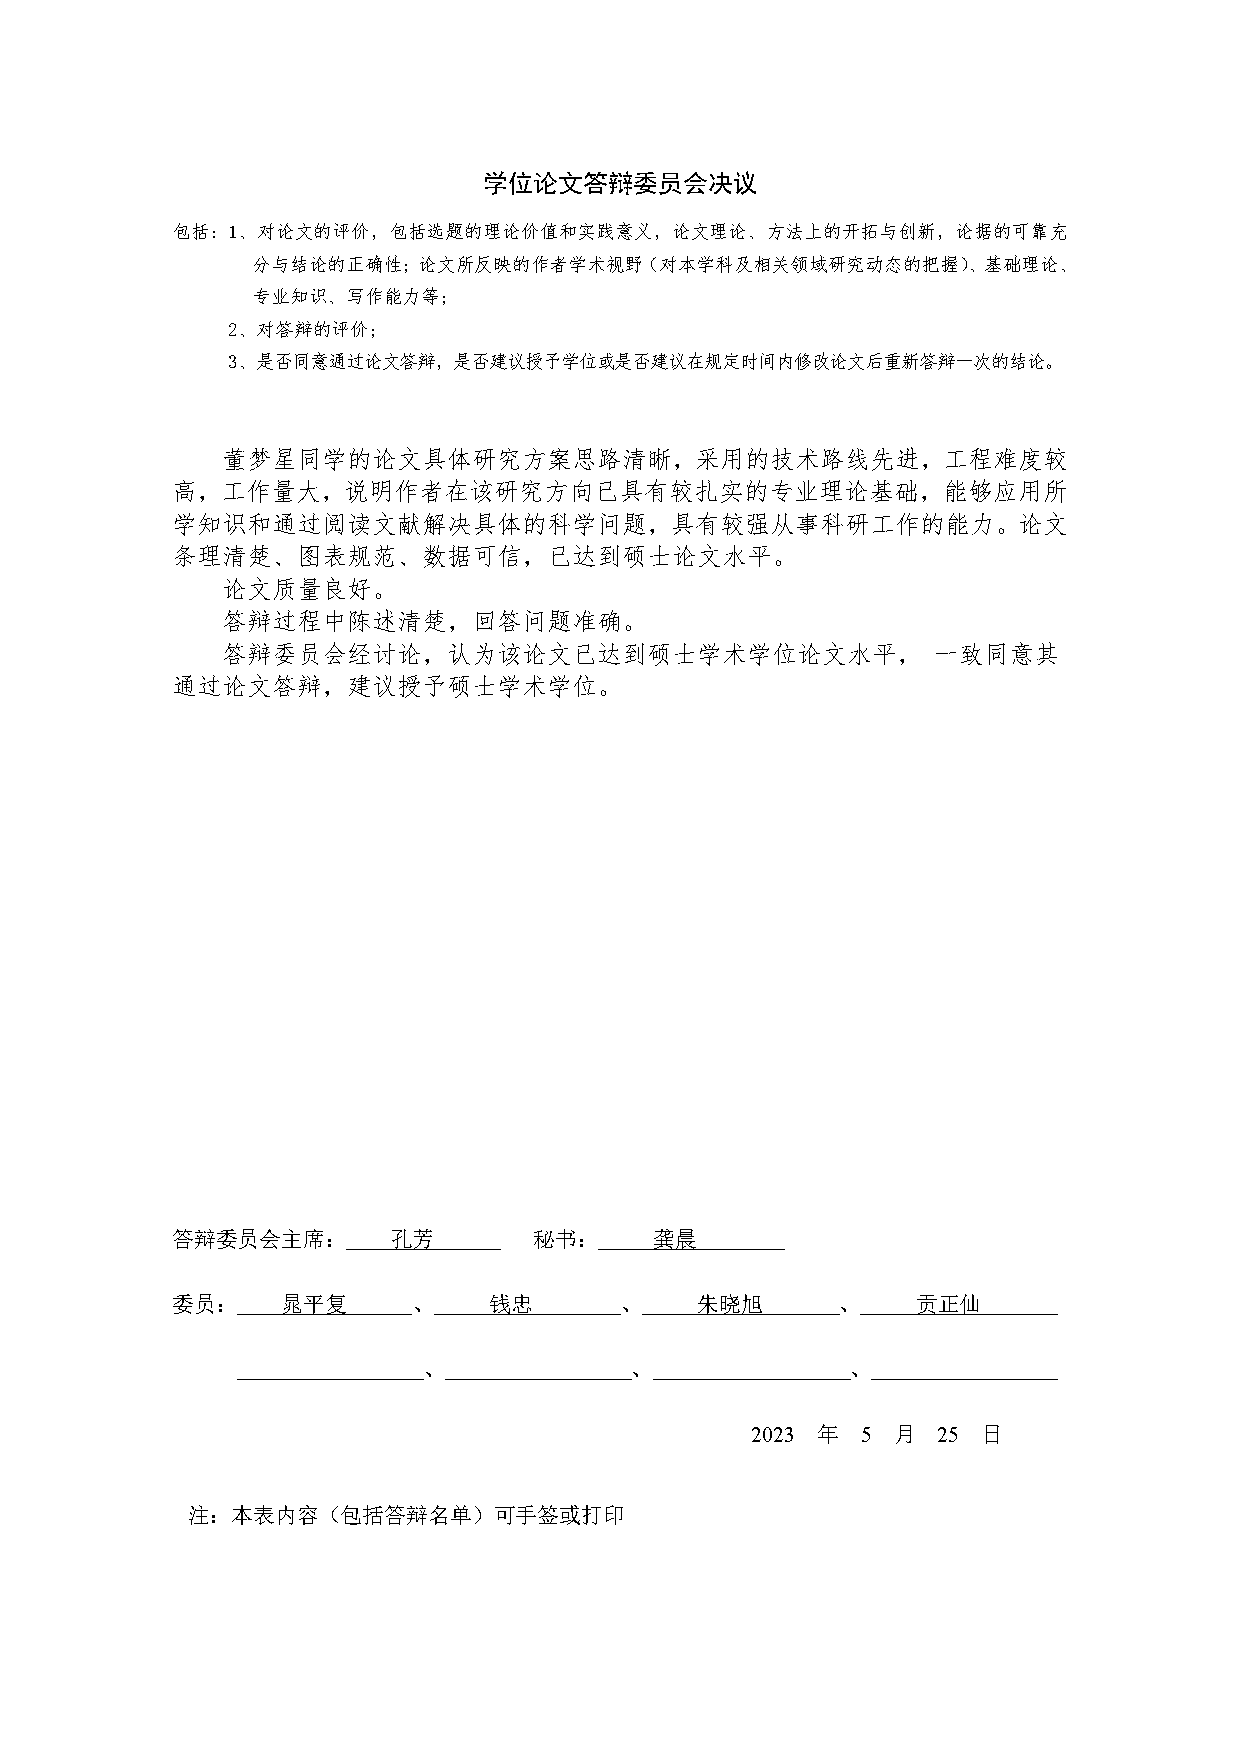
\includepdf[page=-]{pdf-pages/委员会决议.pdf}

\end{document}
